%%% Time-stamp: <mainrep.tex 19:57, 17 Jul 2016 by P Sunthar>
%%% $Log:$
% This document describes how to use iitbreport style
%********************************************************************

%\documentclass[11pt,a4paper,openright]{report}
\documentclass[tikz, twoside]{iitbreport}
% \documentclass[twoside,draft]{iitbreport}

%% Default spacing: 1.5
%% Default font size: 12pt
%% Default font: txfonts (similar to times new roman)

%% Selectively comment out sections that you want to be left out but
%% maintaining the page numbers and other \ref
\includeonly{%
  % intro/introduction,
  % lit/literature,
  % expt/experimental,
  % rnd/results,
  chapter_intro/intro,
  chapter_ctvf/ctvf,
  chapter_csph/csph,
  chapter_implementation_detail/implementation_detail,
  chapter_fsi/fsi,
  chapter_rfc/rfc,
  chapter_erosion/erosion,
  chapter_conclusions/conclusions,
  dec,abs,pub,ack
  % chapter_tmp_misc/guide_to_writing,
}

%%% Some commonly used packages (make sure your LaTeX installation
%%% contains these packages, if not ask your senior to help installing
%%% the packages)
\usepackage{lipsum}
\newcounter{question}
\setcounter{question}{0}

\usepackage{booktabs}
\graphicspath{{expt/}}
\usepackage{cleveref}
\usepackage[hidelinks]{hyperref}

% For the TODOs
\usepackage{xcolor}
\usepackage{xargs}
\usepackage[colorinlistoftodos,textsize=footnotesize]{todonotes}
\newcommand{\todoin}{\todo[inline]}
\usepackage{graphicx}
\usepackage{caption}
\usepackage{subcaption}
\usepackage{algorithm}
\usepackage{algpseudocode}


%%% Macro definitions for Commonly used symbols
\newcommand{\Rey}{\ensuremath{\mathrm{Re}}}
\newcommand{\avg}[1]{\ensuremath{\overline{#1}}}
\newcommand{\tenpow}[1]{\ensuremath{\times 10^{#1}}}
\newcommand{\pder}[2]{\ensuremath{\frac{\partial#1}{\partial#2}}}

% Referencing macros
\newcommand{\Eqref}[1]{Equation~\eqref{#1}}
\newcommand{\Tabref}[1]{Table~\ref{#1}}
\newcommand{\Figref}[1]{Figure~\ref{#1}}
\newcommand{\Appref}[1]{Appendix~\ref{#1}}

%Boldtype for greek symbols
\newcommand{\teng}[1]{\ensuremath{\boldsymbol{#1}}}
\newcommand{\ten}[1]{\ensuremath{\mathbf{#1}}}

% ================= python ===========================
% ================= python ===========================
% ================= python ===========================
% Default fixed font does not support bold face
\DeclareFixedFont{\ttb}{T1}{txtt}{bx}{n}{12} % for bold
\DeclareFixedFont{\ttm}{T1}{txtt}{m}{n}{12}  % for normal

% Custom colors
\usepackage{color}
\definecolor{deepblue}{rgb}{0,0,0.5}
\definecolor{deepred}{rgb}{0.6,0,0}
\definecolor{deepgreen}{rgb}{0,0.5,0}

\usepackage{listings}
\usepackage{minted}

\lstset{language=Python,
  basicstyle=\ttfamily\bfseries\small,
  commentstyle=\color{red}\itshape,
  stringstyle=\ttfamily\color{green!50!black},
  showstringspaces=false,
  keywordstyle=\color{blue}\bfseries}%
% ================= python ===========================
% ================= python ===========================
% ================= python ===========================


% ================= tikz ===========================
% ================= tikz ===========================
\usetikzlibrary{arrows.meta,chains,%
                decorations.pathreplacing}

\usetikzlibrary{matrix,backgrounds}
% ================= tikz ===========================
% ================= tikz ===========================

\begin{document}

%%********************************For question and answer format***********************
\newcommand\Que[1]{%
   \leavevmode\par
   \stepcounter{question}
   \noindent
   \thequestion. Q --- #1\par}

\newcommand\Ans[2][]{%
    \leavevmode\par\noindent
   {\leftskip37pt
    A --- \textbf{#1}#2\par}}

%%********************************Frontmatter***********************
% In frontmatter everything comes with roman numbering
\pagenumbering{roman}
\setcounter{page}{1}

%*******************************************************************
%                         Title Page
%*******************************************************************
\title{Coupled Smoothed Particle Hydrodynamics - Discrete Element Method
  for Fluid and Solid Mechanics}
\author{Dinesh Adepu}

%% Print the date. Today's date comes by default, change it here to
%% other date format, if required:

%\date{\today}
%\date{10 Mar 2016}


%% The type of the report can be set here

% \reporttype{A Seminar Report}
\reporttype{A Thesis}
%\reporttype{A Dissertation}
%\reporttype{A Project Report}

%% Name of the degree
\degree{Doctor of Philosophy}
%\degree{Master of Technology}


%% Department/Centre Name
\dept{Department of Aerospace Engineering}

%% Supervisor and cosupervisor/excosupervisor are not essential parts
%% of a report title page, as it is your report!

%% But if you **have** to put it uncomment these
\supervisor{Prof. Prabhu Ramachandran}
%\cosupervisor{Co-super name}
%\excosupervisor{External Supervisor}

%% Roll number
\rollnum{Roll No. 153010009}

\maketitle

%*******************************************************************
%                         Copyright Page
%*******************************************************************
%\mycopyright

%*******************************************************************
%                         Dedication Page
%*******************************************************************
% \dedication[Dedicated to Nietzsche]
\dedication[To \\ \cdots]
%\addintoc{Dedication}

%*******************************************************************
%                        Certificate Page
%*******************************************************************
%\makecertificate[change title name]{report type}
% \makecertificate{seminar report}
\makecertificate{thesis}
%\makecertificate{dissertation}
%\makecertificate{project report}

%\addintoc{Certificate}

%*******************************************************************
%                         Approval Sheet
%*******************************************************************
\makeapproval{thesis}
%\makeapproval{dissertation}

%*******************************************************************
%                          Declaration
%*******************************************************************
\include{dec}
%\addintoc{Declaration}

%*******************************************************************
%                        Acknowledgements
%*******************************************************************
%%%
\acknowledgments


Firstly, I thank my supervisor Prof. Prabhu Ramachandran for giving me an
opportunity to pursue the Ph.D. program under him. I am very thankful for all
his support throughout my stay at IIT Bombay and the freedom to pursue my
interests in different fields.

I thank Prof. Chandra Shekar for his help. I thank my colleague Abhinav Muta for
his help and for all the excellent discussions we had throughout our stay at IIT
Bombay. I want to thank Pawan Negi for his invaluable technical discussions. I
thank Vinay Narasimhan for his support in providing me with all the resources to
run my simulations on time. I thank my research committee member, Prof. Manaswita
Bose for her valuable comments and advice.


A special mention to a few people at IIT Bombay for making my stay here very
memorable, Jagadeesh Babu Vemula, Praveen Kumar Kanduri, Ananya Aishwarya,
Singham Naresh. I thank all my family members for their support.

I thank a few living and non-living mentors, without whom this Ph.D. wouldn't be
possible. Friedrich Nietzsche, Ayn Rand, Schopenhauer, Novak Djokovic, and Sir
Lewis Hamilton, from whom I took constant inspiration throughout my Ph.D.


\signature{\today}
%\signature[Indian Institute of Technology Bombay]{\today}

%========================================================================

%%% Local Variables:
%%% mode: latex
%%% TeX-master: "../mainrep"
%%% End:


%******************************************************************
%                          Abstract
%******************************************************************
%============================= abs.tex================================
\begin{Abstract}
  In the present work, we develop a coupled formulation of Smoothed Particle
  Hydrodynamics (SPH) - Discrete Element Method (DEM) to handle fluid and solid
  mechanics problems. The framework is applied to model several different types
  of physics, such as fluid dynamics, elastic-plastic dynamics, rigid body
  dynamics, rigid-fluid coupling (RFC), fluid-structure interaction (FSI), and
  solid particle erosion (SPE). Applications such as abrasive water jet
  machining, fluid-bed reactors, and sediment transport are a few areas where
  these physical phenomena are dominant. We use SPH to model the fluid and
  elastic-plastic dynamics, while DEM handles the interaction among the
  arbitrarily shaped bodies. We implement the current work in the open-source
  framework PySPH. We use an automan package to automate all our results and
  make it fully reproducible. We produce an open-source framework of
  the current formulation in handling all these different physical processes.


  We first develop a technique in SPH to model fluid and elastic dynamics.
  Particle shifting techniques (PST) in SPH have been used to improve the
  accuracy of the SPH method. Shifting ensures that the particles are
  distributed homogeneously in space. This may be performed by moving the
  particles using a transport velocity. In this work, we propose an extension
  to the class of Transport Velocity Formulation (TVF) methods. We derive the
  equations in a consistent manner and show that there are additional terms that
  significantly improve the accuracy of the method. In particular, we apply this
  to the Entropically Damped Artificial Compressibility SPH method. We identify
  the free-surface particles and their normals using a simple approach and
  thereby adapt the method for free-surface problems. We show how the new method
  can be applied to the problem of elastic dynamics. We consider a suite of
  benchmark problems involving both fluid and solid mechanics to demonstrate the
  accuracy and applicability of the method.

  We extend the CTVF technique to handle the collision among the frictional
  elastic solids using a contact force model. Classically, smoothed particle
  hydrodynamics (SPH) is used to model collision between elastic solids, which
  involves handling the deformation of bodies and the interaction with other
  bodies. However, this does not allow one to incorporate friction and also
  subjects the solids to unphysical interaction when the bodies are nearby but
  not in actual contact. In the current work, we incorporate an efficient
  contact force model into a variant of the updated-Lagrangian SPH to model the
  interaction between elastic solids. This approach models friction as well as
  eliminates the spurious interaction between nearby bodies. The current model
  is validated with several numerical examples involving a collision between two
  and multiple elastic solids, with and without friction. These results compare
  well with finite element modeling (FEM), analytical, and experimental studies.
  We discuss the implementation details of contact force formulation to handle contact
  between the colliding bodies in PySPH. The model is easy to incorporate in any
  updated-Lagrangian SPH scheme.


  We further study the deformation of elastic structures under hydrodynamic
  loads with the CTVF model. CTVF is adopted to handle both fluid and structural
  dynamics, as it can eliminate inhomogeneous particle distribution in fluid
  flow and tensile instability in elastic structures without any additional
  terms. A ghost particle-based approach is used to handle the coupling between
  the fluid and solid phases. The proposed scheme is verified by simulating a
  few test cases, which are validated with exact analytical solutions. An
  elastic plate deformation due to dam-breaking fluid is simulated as an
  application. We outline sub-stepping algorithm used to update the states of
  two different materials for computationally efficient simulation.

  Next, we study the two-way coupling between the rigid body and the fluid flow
  using a particle-based framework. The interaction between the rigid bodies is
  handled with the discrete element method (DEM), where the contact force model
  developed to handle the collision between arbitrarily shaped elastic solids is
  used. The fluid phase is modeled with CTVF. The interaction between the fluid
  and rigid bodies is modeled using a dummy particle approach which is similar
  to handling the interaction between the fluid and the elastic structure. The
  accuracy of the developed method is evaluated via several numerical examples
  involving analytical and experimental results. The rigid-rigid interaction
  part of the solver is validated through the study of rolling and sliding body
  cases. The collapse of a stack of cylinders under gravity is studied and
  compared against its experimental counterpart. The rigid-fluid interaction is
  studied with the water entry of a rigid cube and with a rising cylindrical body
  case in the hydrostatic water tank.

  We finally model the erosion of a ductile solid due to the impact of multiple
  arbitrarily shaped projectiles. We model the elastic-plastic behavior of the
  ductile solid by incorporating a Johson-Cook constitutive model in CTVF. We
  adapt the contact force between the elastic bodies formulation to
  rigid-elastic solids. We further build a framework that can handle erosion of
  the target due to the impact of multiple bodies, which can interact or do not
  interact among themselves. 2D and 3D numerical cases are simulated to
  demonstrate the developed framework abilities. Erosion of a 2D ductile target
  due to multiple square particle impacts, with cases where square particles can
  self-interact and with no self-interaction, is simulated. A rotating spherical
  particle impacting a ductile target at different impact velocities is
  considered part of the 3D case.

%
%
%
%
%
\end{Abstract}
%=======================================================================


%******************************************************************
%                         Contents list
%******************************************************************
%\figurespagefalse
%\tablespagefalse
\makecontents % Creats toc, lof, and lot

%******************************************************************
%                        Notations
%******************************************************************
\notations[4cm]{List of Symbols}

%%********************************Mainmatter***********************
% In mainmatter everything comes with arabic numbering
\cleardoublepage
\setcounter{page}{1}
\pagenumbering{arabic}

%******************************************************************
%                         Chapters
%******************************************************************
% \include{intro/introduction}
% 
\chapter{Literature Survey}

The bibliographic entries are to be kept in a file named
\verb|<something>.bib|. In this sample report we call it as
\verb|mylit.bib|. This file must be included without the \verb|.bib|
extension in the main file as: \verb|\bibliography{mylit}|.   Open the
file \verb|mylit.bib| to see the format in which the entries are
written. This is written in the Bib\TeX format. Most of the
bibliographic web pages (Scopus, ISI Web) and software (EndNote, etc)
allow you to export bibliographic entries in the Bib\TeX format.

Citations are referred in the text using \verb|\citet| command which produces citations as though they are part of the text.  In order to say
somebody did this work as a part of a line use:
\verb|\textcite{Batzri1973}| have done extensive work on \ldots.  This will produce
\textcite{Batzri1973} have done extensive work on \ldots. Alternately citations can appear in parenthesis.
The command~\verb|\parencite{Batzri1973}| is used to automatically put the
citations in parenthesis.  As an example consider the extensive work
done in the area of book writing \parencite{Sackmann1995a,Boal2012}.

Conferences \parencite{rich-mart92} or collection of work
\parencite{Sackmann1995a} also have special entries.

It is also possible to cite thesis like this:
\textcite{jariwala00,luding94} or just unpublished work from
\textcite{SunHI03}. Some times there are unclassified bibliographic
entries which can be put under ``misc'' \parencite{Smith99}.



%%% Local Variables: 
%%% mode: latex
%%% TeX-master: "../mainrep"
%%% End: 

% \include{expt/experimental}
% \include{rnd/results}
\chapter{Introduction}
\label{chap:SPH}

\section{Abrasive water jet machining}
Material erosion with a high-pressure water jet with abrasives is widely found
in the industry applied to design machining of
metals~\citep{llanto_recent_2021}, composites~ \cite{alberdi_composite_2013}.
Such machining is widely known as abrasive water jet machining (AWJM). AWJM is
used for cutting metallic sheet, glass, and composite materials for automobile,
housing, and aircraft
industries \citep{alberdi_composite_2013,aich_abrasive_2014,llanto_recent_2021},
respectively.
\begin{figure}
  \centering
  \includegraphics[width=0.5\textwidth]{images/intro/images/intro_section/big_picture}
  \caption{}
\label{fig:intro-big-picture}
\end{figure}
\Cref{fig:intro-big-picture} describes the erosion of brittle solid due to the
impact of rigid bodies in a fluid flow. To model AWJM accurately, we need to
model the incoming fluid dynamics, elastic-plastic behavior of the target, rigid
body dynamics of the impactor, collision handling among the impactors and
between the impactor and the target, two way coupling between the fluid flow and
impactor, and the elastic structure, called as fluid-structure interaction. An
analytical study of AWJM is not possible as it is highly nonlinear and involves
several different multi-physical processes. Therefore, we choose numerical
modeling due to its flexibility in handling nonlinear behavior. Test cases with
exact analytical solutions and experimental cases can be used to develop
numerical techniques while handling each physical process. Mesh-based and
meshless techniques are used to model the AWJM numerically.


% \textbf{Write about SPH and why we choose SPH, about software, updated
%   Lagrangian open source, DEM, runs on all architectures}.


\section{State of the art}

\subsubsection*{Modeling of fluid and elastic dynamics in SPH}

The smoothed particle hydrodynamics (SPH) method has been widely applied since
it was originally proposed to simulate hydrodynamic problems in astrophysics
independently by \citet{lucy77}, and \citet{monaghan-gingold-stars-mnras-77}. It
has been extensively applied to simulate problems involving
fluids~\citep{dalrymple2001sph,shao2003incompressible} in particular to both
compressible~\citep{monaghan-review:2005}, incompressible fluid
flows~\citep{sph:fsf:monaghan-jcp94,sph:psph:cummins-rudman:jcp:1999} as well as
elastic dynamics problems~\citep{randles-1996,gray-ed-2001}, fluid-structure
interaction \citep{khayyer2018enhanced,he2017coupled}, granular physics
\citep{bui2008lagrangian,bui2021smoothed} among other areas.
\cite{monaghan2012smoothed} provides a detailed review of SPH and its
applications.

% in addition to a
% variety of other problems~\citet{rafiee:fsi-2009,khayyer-fsi-2018,
%   sun2021accurate, bui2008lagrangian}.


% The SPH method is a meshless numerical method originally proposed by
% \cite{gingold1977smoothed} and \cite{lucy1977numerical} to model
% astrophysics problems. structural dynamics \citep{randles1996smoothed,dong2016smoothed},



The SPH method is meshless and Lagrangian, and therefore particles move with the
local velocity. This motion can introduce disorder in the particles and thereby
significantly reduce the accuracy of the method. \cite{acc_stab_xu:jcp:2009}
proposed an approach to shift the particles so as to obtain a uniform
distribution of particles. This significantly improves accuracy and the method
is referred to as the Particle Shifting Technique (PST). Many different kinds of
PST methods are available in the
literature~\citep{diff_smoothing_sph:lind:jcp:2012,fickian_smoothing_sph:skillen:cmame:2013,huang_kernel_2019,ye2019sph}.
An alternative approach that ensures particle homogenization for incompressible
fluid flow was proposed as the Transport Velocity Formulation
(TVF)~\citep{Adami2013}. The method introduced an additional stress term to
account for the motion introduced by the particle shifting. The TVF produces
very accurate results but only works for internal flows. \cite{zhang_hu_adams17}
proposed the Generalized Transport Velocity Formulation (GTVF) thereby allowing
the TVF to be used for free-surface problems as well as elastic dynamics
problems. This allows for a unified treatment of both fluids and solids.
Similarly, \cite{oger_ale_sph_2016} introduce ideas from a consistent ALE
formulation for improving the accuracy of SPH. They employ a Riemann-based
formulation to solve fluid mechanics problems and introduce particle shifting to
obtain highly accurate simulations for internal and free-surface problems may
also be handled. The PST has also been employed in the context of the
$\delta$-SPH schemes\citep{sun_consistent_2019}.


The Entropically Damped Artificial Compressibility SPH scheme
(EDAC-SPH)~\citep{edac-sph:cf:2019} introduces an evolution equation for the
pressure and significantly reduces the noise in the pressure since it features
a pressure diffusion term. The approach has a thermodynamic
justification~\citep{Clausen2013} and produces very accurate
results~\citep{edac-sph:cf:2019}.


Recently, \cite{antuono2021delta} carefully combine the ALE-SPH method of
\cite{oger_ale_sph_2016} and the consistent $\delta$-SPH formulation of
\cite{sun_consistent_2019} to improve the accuracy of the $\delta$-SPH
method. They show the importance of the additional terms to the accuracy.


Modeling of elastic solids in SPH was first proposed by
\cite{libersky1991smooth}, where the authors studied the high-speed impact
problems. Despite SPH being applied to elastic solid modeling, it suffers from
tensile instability~\citep{swegle1995smoothed}. The tensile instability problem
has given rise to the total Lagrangian SPH \citep{bonet2002alternative,
  vignjevic2006sph, belytschko2000unified}, where the derivatives of particle
properties are computed in the reference configuration using the deformation
gradient. The updated Lagrangian approach is used by \cite{gray2001sph} and
\cite{monaghan2000sph} where an artificial stress term is introduced to control
instabilities. Many other variants of the updated Lagrangian SPH have been
proposed. Godunov SPH \citep{sugiura2017extension} utilizes a Riemann solver to
reduce the usage of artificial viscosity and a new equation of state is
formulated to solve the tensile instability problem. \cite{dyka1995approach}
uses two sets of particles, where one set of particles stress is computed, and
the other set of particles are used for the evolution of other properties,
through which the tensile instability has been overcome.
\cite{zhang2017generalized} extended the transport velocity formulation (TVF) of
\cite{adami2013transport} to structural dynamics problems and free-surface fluid
mechanics problems. Here the particles are moved with a transport velocity
rather than the momentum velocity to ensure a more homogeneous particle
distribution. This approach also solves the tensile instability problem.


\subsubsection*{Collision SPH}
The dynamics of the projectiles can be modeled by assuming the bodies to be
rigid, as done in the discrete element method (DEM) (\citep{zhan2021surface}).
However, this does not consider any elastic or elastic-plastic deformations of
these colliding bodies. In these cases either finite element methods (FEM)
\citep{rodrigues2019elastic} or meshless methods such as material point
method\citep{sulsky1994particle} or smoothed particle hydrodynamics (SPH)
\citep{gingold1977smoothed} can be used. In this context meshless methods, such
as the SPH method, are advantageous when modeling large deformation of solids as
they do not suffer from issues such as mesh entanglement.

SPH has been successful in modeling the collision between the elastic as well as
elastic-plastic solids \citep{gray2001sph, cleary2010elastoplastic}.
\cite{yan2021simulation} introduced the interfacial SPH scheme, where the SPH
forces are computed only within each body but the interaction between two bodies
is computed using a repulsive force inspired from ABAQUS.
\cite{vyas2021collisional} has modeled the interaction between a rigid body with
an elastic solid, using a penalty-based contact force model.
\cite{mohseni2021particle} use a contact model in order to simulate the
collision between non-smooth rigid bodies with elasto-plastic targets. In both
\citep{vyas2021collisional} and \citep{mohseni2021particle} the friction between
the rigid body and target is considered.


\subsubsection*{Fluid-structure interaction}
The interaction between the ductile target and the incoming jet can be
considered as a fluid-structure interaction phenomenon. Mesh-based schemes such
as finite element method (FEM) \citep{lozovskiy2015unconditionally} and finite
volume method (FVM) \citep{jasak2007updated} have been used for the last few
decades in modeling the FSI problems. However, mesh-based methods are not
favorable when dealing with free surface flow problems or problems involving
large deformation of the structure. This is due to explicit free surface
tracking, and mesh distortion \citep{moresi2003lagrangian} while dealing with
large deformation solids. Therefore, meshless methods are preferred while
handling FSI problems involving free surfaces, multiphase flows, and large
deformation in solids. The smoothed particle hydrodynamics (SPH) and material
point method (MPM) are more commonly used to model the fluid phase. While the
solids are modeled with SPH or Reproducing Kernel Particle Methods (RKPM), or
the Discrete Element Method (DEM) \citep{hu2010material,li2022material}. These
meshless techniques have been coupled for the past two decades to model the
fluid-structure interaction. A few schemes with SPH and MPM are SPH-DEM~
\citep{wu2016coupled}, SPH-TLSPH~\citep{salehizadeh2022coupled},
SPH-RKPM~\citep{peng2021coupling}, SPH-Peridynamics~\citep{sun2020smoothed},
MPM-DEM~\citep{singer2022partitioned}. For more, see the review by
\citep{khayyer2022systematic}.



\subsubsection*{Rigid-fluid coupling and rigid-rigid interaction}
Assuming the incoming projectiles as rigid bodies, the influence of rigid body
on the incoming jet and vice versa is modeled as rigid fluid coupling. In rigid
fluid coupling problems, mesh-based schemes \citep{dettmer_computational_2006}
have been in practice to model fluid dynamics for several decades. However,
these schemes are unfavorable when dealing with free surface flows and mediums
undergoing huge deformation \citep{walkley_finite_2005}. Meshless methods have
been advantageous in modeling free surfaces and large deformations problems.
Therefore, meshless techniques are preferred in addressing these problems. Among
many meshless techniques, moving particle semi-implicit (MPS) - discrete element
method (DEM) \citep{guo2017numerical} and smoothed particle hydrodynamics
(SPH)-DEM \citep{canelas2016sph} are two coupling strategies used to handle
rigid-fluid coupling problems. The rigid body interaction is modeled with DEM.
In addition to DEM, works where SPH \citep{amicarelli2015smoothed} is used to
model the rigid-rigid interaction. However, it lacks to incorporate the friction
between the bodies. MPS and SPH are used to model the fluid phase, and a
coupling strategy is utilized to model the interaction between the rigid body
and the fluid phase.

\cite{cundall_discrete_1979} proposed DEM to study discrete granular materials.
In DEM, the particle dynamics follow simple Newtonian force laws and interact at
their surfaces through a contact force. A shape, mass, and moment of inertia are
assigned to each particle, and originally the particles are assumed to have a
spherical shape. Variations of the DEM were proposed to handle bodies with
different shapes, such as dilated polyhedral DEM \cite{liu_new_2020}, Fourier
series-based discrete element method \cite{lai_fourier_2020}
Gilbert-Johnson-Keerthi(GJK)-DEM \citep{wachs2012grains3d}, discrete function
representation based DEM \citep{lu2012critical}, level set DEM method
\citep{duriez2021precision}. Interaction between bodies with irregular
geometries is modeled by multi-sphere approach \citep{kruggel-emden_study_2008},
surface mesh represented(SMR)-DEM ~\cite{zhan2021surface}.


\subsubsection*{Solid particle erosion}

In theoretical studies, \cite{finnie1972some}, \cite{bitter1963study}
studied the surface erosion of ductile and brittle materials. An analytical
expression for the material removal at different angles of impact is derived in
these studies. Further, an analytical study is carried out by
\cite{hutchings1977erosion}, who provides various results relating the
crater depth, erosion rate related to the impactor particles. In numerical
modeling, mesh based methods are in use for the past few decades in modeling the
solid particle erosion. \cite{molinari2002study,takaffoli2009finite} has
studied the single impact problem using FEM. Meshless techniques are been used
in studying the erosion process, this is due to its advantage in handling
problems with large deformation. \cite{dong2016smoothed} uses smoothed
particle hydrodynamics (SPH) to model the erosion of a ductile target.


\section{Motivation}

\subsubsection*{Numerical modeling of fluid and elastic dynamics in SPH}
SPH in modeling fluid and structural dynamics. Faces several issues and many
different additions were proposed to solve the issues. Transport velocity
formulation is used extensively to solve the particle homogenization problems.
With the notable exception of the GTVF scheme~\citep{zhang_hu_adams17}, most
other applications of the PST have been in the context of fluid mechanics. The
GTVF method provides a unified approach to solve both weakly-compressible fluids
as well as solids. However, the method suffers from a few issues. In order to
work for free-surface problems the method relies on using a different background
pressure for each particle and introduces a few numerical corrections to work
around issues. For example, the smoothing length of the homogenization force is
different from that used by the other equations and this parameter is somewhat
ad-hoc. For solid mechanics problems the method uses the transport velocity of
the particle rather than the true velocity in order to compute the strain and
rotation tensor. In addition there are some terms in the governing equations
that are ignored which play a major role. We also note that the method is not
robust to a change in the particle homogenization force. The EDAC-SPH method
uses the TVF formulation for internal flows and for free-surface flows it does
not employ any form of particle shifting.


\subsubsection*{Elastic solids collision}

Though, SPH~\citep{gray2001sph} has been successful in modeling the collision
between the elastic solids, it does not consider friction between the colliding
solids. Another problem is that the model generates spurious forces on bodies
which are moving close to each other (within the influence radius of the SPH
particles) but not actually interacting. \cite{yan2021simulation} introduced the
interfacial SPH scheme, which eliminates the spurious interactions but it can
not handle friction between the solids. The interaction force does not consider
the shape of the solids in contact. \cite{mohseni2021particle} models the
interaction between a rigid body and a ductile solid using a contact force
model, where the bodies are divided as being primary and a secondary. In
\citep{mohseni2021particle}, the primary body is usually treated as the rigid
body and the body on which the erosion is simulated is treated as secondary.
\cite{vyas2021collisional} also consider the collision between a rigid and
elastic body. \cite{vyas2021collisional} where too there is a clear distinction
between primary and secondary bodies. It is not clear what would happen if both
bodies were elastic or if there is no clear way to distinguish between a primary
and secondary body. \cite{vyas2021collisional,mohseni2021particle} works are not
applied to model the interaction between elastic solids.


\subsubsection*{Fluid-structure interaction and rigid-fluid coupling}
The dynamics of the interaction between ductile target and the incoming jet is
considered as fluid-structure interaction. With meshless techniques preferred in
free surface and large deformation problems. Several different meshless
techniques are coupled in order to simulate the FSI phenomenon. FSI in SPH alone
is modeled by several works, such as, WCSPH-Total Lagrangian SPH (TLSPH)
\citep{zhan2019stabilized}, WCSPH-Updated Lagrangian SPH (ULSPH)
\citep{antoci2007numerical}, ISPH-TLSPH\citep{salehizadeh2022coupled}. However,
using only an updated Lagrangian framework with transport velocity formulation
no work is reported in modeling FSI.

Movement of arbitrarily shaped rigid projectiles are modeled using a
multi-sphere and SMR-DEM approach. However, multi-sphere approach fails to
handle the contact accurately with bodies involving sharp corners, as the force
law assumes the contact between two spherical particles. SMR-DEM requires
additional information to handle the collision, such as connectivity between the
particles comprising the body in addition to the particle positions. However, we
need additional sets of particles to handle the interaction between the rigid
body and the fluid particles. \cite{mohseni2021particle} proposed a new contact
force law, which handles the collision between the bodies based on particle
positions alone. Here the amount of overlap between the bodies is computed using
an SPH method. Utilizing \citep{mohseni2021particle} to model contact between
the bodies allows us to handle the interaction between the fluid particles with
the same set of particles in contrast to SMR-DEM ~\cite{zhan2021surface}.
However, \citep{mohseni2021particle} is applied to contacts involving rigid and
a ductile solids. \citep{mohseni2021particle} is not applied to model the
interaction between inelastic rigid bodies, and in problems involving fluids.


\subsubsection*{Solid particle erosion}
FEM~\citep{takaffoli2009finite} is successful in modeling solid particle
erosion, however, it fails to model the erosion due to many particles. Further,
FEM is not suitable for modeling multiphysics problems, as AWJM has rigid fluid
coupling, FSI in addition to modeling fluid and elastic dynamics.
\cite{dong2016smoothed} uses smoothed particle hydrodynamics (SPH) to model the
erosion of a ductile target. However, \cite{dong2016smoothed} does not consider
the arbitrary shape of the projectile. Further, collision among the projectiles
while interacting with the target is not modeled in SPH. To the authors
knowledge there is no open-source implementation in the literature which can
model the solid particle erosion in SPH.

To develop an open-source framework to model the physics involved in AWJM in SPH.
The following are the key goals of the work.
\begin{itemize}
\item Develop a unified technique in SPH to solve both fluid and solid dynamics
  problems.
\item Handle the collision between the elastic solids using a penalty-based contact force.
\item Develop a fluid-structure interaction solver.
\item Handle the collision among the arbitrarily shaped rigid projectiles in fluid
  flow. Solve the two-way coupling between the fluid and the rigid bodies.
\item Provide an open-source implementation for solid particle erosion in SPH.
\end{itemize}


In this work we propose a scheme which we called Corrected Transport Velocity
Formulation (CTVF) that is inspired by the various recent developments but is
consistent and which works for both solid mechanics and fluid mechanics
problems. We derive the transport velocity equations afresh and note that
there are some important terms that are ignored in earlier approaches using
TVF. These terms are significant and improve the accuracy of the method.
Similar to \cite{oger_ale_sph_2016,sun_consistent_2019}, we detect the free
surface particles and compute their normals using a simpler and
computationally efficient approach which does not require the computation of
eigenvalues. This allows the method to work with free-surfaces without the
introduction of numerical parameters or a variable background pressure. We
employ the EDAC formulation and show that there are additional correction
terms in the EDAC scheme that should be introduced to improve the accuracy of
the method. Furthermore, we show how the EDAC scheme can be used in the
context of solid mechanics problems. We make use of the particle velocity
rather than the transport velocity to compute the velocity gradient, strain,
and rotation rate tensors. Our method can be used with any PST and we consider
the method of \citet{sun_consistent_2019} as well as the iterative PST of
\citet{huang_kernel_2019}. The method is also robust to the choice of the
smoothing kernel. The resulting method works for both weakly-compressible
fluids as well as solids. The new method may be thought of as an improved
extension of the EDAC-SPH method that can be used for free-surface problems as
well as solid mechanics problems.


In the current work, the collision between elastic solids is modeled using a
penalty-based contact force model. Unlike the approach of
\cite{yan2021simulation}, the proposed contact force model can handle friction
between the solids as well. The bodies themselves are elastic and this is
simulated using the CTVF SPH method \cite{adepu2021corrected}. The penalty-based
force considered here is the one proposed by \citet{mohseni2021particle}. In the
original model proposed by \cite{mohseni2021particle}, the contact force is
between a primary body and a secondary body. In \cite{mohseni2021particle}, the
primary body is usually treated as the rigid body and the body on which the
erosion is simulated is treated as secondary. It is not clear what would happen
if both bodies were elastic or if there is no clear way to distinguish between a
primary and secondary body. We explore the importance of choosing the primary
and secondary body under collision.

In the current work, we handle FSI problems by the CTVF method, where both
fluids and solid phases are modeled using CTVF alone. We couple CTVF with DEM to
model the rigid fluid coupling problems. The fluid phase is handled using a
corrected transport velocity formulation developed by \cite{adepu2021corrected},
which provides smooth pressure distribution with EDAC formulation and
homogeneous particle distribution, resulting in accurate fluid modeling. While
DEM is used to handle rigid-rigid interactions and applied to 3D problems, and
it is further modified to handle inelastic collisions by introducing a damping
term in the contact force equation. The interaction between the fluid phase and
rigid bodies is handled using the dummy particle approach \citep{Adami2012}.


\section{Overview}
The current thesis is organized in the following way. The current chapter
introduces the basic formalism of SPH. In the next chapter, \cref{chap:ctvf}, we
introduce corrected transport velocity formulation in SPH and apply it to model
the dynamics of fluids and elastic structures. The new formulation eliminates
several issues SPH faces. \Cref{chap:csph} improvises the collision model by
incorporating a contact force model in SPH while the bodies are colliding. This
essentially eliminates spurious interaction between the bodies and incorporates
friction between the interacting bodies. \Cref{chap:fsi} is utilized to model
the interaction between the elastic structure and the incoming jet. This is
modeled with coupling the solver developed in \cref{chap:ctvf}, here both fluid
and solid phases and coupled using a dummy particle approach. In
\cref{chap:rfc}, we study the dynamics of the projectiles onto the target in an
incoming high-speed jet. We couple CTVF with DEM to model the rigid fluid
coupling phenomenon. The interaction between the rigid bodies is handled with
DEM. \Cref{chap:erosion} models the solid particle erosion of the ductile body
due to an impact of the projectile. The contact force implemented in
\cref{chap:csph} is used to handle the interaction between the rigid body and
the ductile solid. Johnson-Cook constitutive model is utilized to model the
plasticity of the target.


In the next section we introduce the SPH methodology and show how a function,
derivative and divergence operators are approximated.
% We show how SPH is used to
% solve the fluid and elastic solid problems in updated Lagrangian formalism.
% Several issues of SPH is discussed, tensile instability, particle
% inhomogenization, through numerical examples.

\section{Smoothed particle hydrodynamics}
In the current section, we introduce the basics of smoothed particle
hydrodynamics. A fundamental overview of the discrete approximations of
function, derivative, and divergence is discussed. Advanced approximations are
derived, keeping the conservation of quantities in mind.
\subsection{Function approximation}
The function value of a smooth function $A$ defined over a domain $\Omega$ at
point $x$ can be written as
\begin{equation}
  \label{eq:dirac_repr}
  A(\ten{x}) = \int_{\Omega}\> A(\ten{x}') \> \delta(\ten{x} - \ten{x}') \> d\ten{x}'^{n},
\end{equation}
where $\delta(\ten{x} - \ten{x}')$ is a Dirac-delta function having the
following properties,
\begin{equation}
  \label{eq:dirac-delta}
  \delta(\ten{x}) =
  \begin{cases}
    +\infty, & \ten{x} = \ten{0}\\
    0, & \ten{x} \neq \ten{0}
  \end{cases}
\end{equation}
and
\begin{equation}
  \label{eq:unity}
  \int_{\Omega}\> \delta(\ten{x}) \> d\ten{x} = 1.
\end{equation}
Here, $m$ chosen depending on the dimension of the space, $2$ and $3$ for 2D and 3D space.
The exact function value at $x$ can be retrieved by the following steps,
\begin{align*}
  \label{eq:dirac_derivation}
  A(\ten{x}) &= \int_{\Omega}\> A(\ten{x}') \> \delta(\ten{x} - \ten{x}') \> d\ten{x}'\\
  A(\ten{x}) &= A(\ten{x}) \int_{\Omega}\> \> \delta(\ten{x} - \ten{x}') \> d\ten{x}'\\
  A(\ten{x}) &= A(\ten{x})
\end{align*}
In SPH, the Dirac delta function is replaced with a compact smooth function $W$,
chosen to be as even function. The function value of $A$ at $\ten{x}$
interpolated with the smooth kernel $W$ is given by
\begin{equation}
  \label{eq:kernel_repr}
  A(\ten{x}) = \int_{\Omega}\> A(\ten{x}') \> W(\ten{x} - \ten{x}', h)  \> d\ten{x}' + O(h^2).
\end{equation}
Here, kernel $W$ satisfies the unity condition, given by
\begin{equation}
  \label{eq:unity}
  \int_{\Omega}\> W(\ten{x} - \ten{x}', h)  \> d\ten{x}' = 1.
\end{equation}

\begin{equation}
  \label{eq:kernel_delta}
  \lim_{h \to 0} W(\boldsymbol{x} - \boldsymbol{x}', h) = \delta(\boldsymbol{x} - \boldsymbol{x}', h)
\end{equation}
\begin{equation}
  \label{eq:compact_support}
  W(\boldsymbol{x} - \boldsymbol{x}', h) = 0 \>\>\>\>    \text{when}  \>\>\> |\boldsymbol{x} - \boldsymbol{x}'| > kh
\end{equation}
In the current work we have used Quintic spline in all our simulation cases. Quintic spline is given as,
\begin{equation}
  \label{eq:quintic_spline}
  W(r, h) =
  \begin{cases}
    \sigma_5\left( (3-q)^5 - 6(2-q)^5 + 15(1-q)^5 \right), & \textrm{for} \ 0\leq q \leq 1,\\
    \sigma_5\left( (3-q)^5 - 6(2-q)^5 \right), & \textrm{for} \ 1 <  q \leq 2,\\
    \sigma_5 \ (3-q)^5 , & \textrm{for} \ 2 < q \leq 3,\\
    0, & \textrm{for} \ q>3,
  \end{cases}
\end{equation}


This type of interpolation leads to a 2nd order function accuracy (cite
references). Much better kernels can be used to approximate the function, but
that may result in negative density which we want to avoid.

Assume that the domain is discretized into N particles with mass $m_i$ and volume
$dv_i$. We have
\begin{equation}
  \label{eq:mass_repr}
  m_j = dv_i \> \rho_i
\end{equation}

Using \eqref{eq:mass_repr}, \eqref{eq:kernel_repr} is converted to
discrete form as follows

\begin{equation}
  \label{eq:discrete_form}
  A_i = \sum\> \frac{m_j}{\rho_j} A_j\> W(\ten{x}_i - \ten{x}_j, h)
\end{equation}

Where $A_i$ is the value of the field property of particle i,
similarly for $A_j$.

\subsection{Derivative approximation}
Similarly, the continuous SPH interpolation of the derivative of a field variable
is written as
\begin{equation}
  \label{intro:eq:sph-continu-derivative-interpolation}
  \nabla A(\ten{x}) = \int_{\Omega}\> \nabla A(\ten{x}') \> W(\ten{x} - \ten{x}', h)  \> d\ten{x}'^{m}
\end{equation}
By applying integration by parts to the right hand side results in,
\begin{equation}
  \label{eq:sph-continu-derivative-interpolation}
  \nabla A(\ten{x}) = - \int_{\Omega}\> A(\ten{x}') \> \nabla_{\ten{x}'} W(\ten{x} - \ten{x}', h)  \> d\ten{x}'^{m} +
  - \int_{\Omega}\> \nabla \left( A(\ten{x}') \> W(\ten{x} - \ten{x}', h)\right)  \> d\ten{x}'^{m}
\end{equation}
From symmetric property of the kernel $W$, we get the derivative of the kernel
as antisymmetric and thus
\begin{equation}
  \label{intro:eq:sph-kernel-antisymmetric}
  \nabla_{\ten{x}'} W(\ten{x} - \ten{x}', h) = -\nabla_{\ten{x}} W(\ten{x} - \ten{x}', h)
\end{equation}
Furthermore, using the Stokes theorem, the last term of
\cref{eq:sph-continu-derivative-interpolation} can be written as a surface
integral, the resulting equation is
\begin{equation}
  \label{intro:eq:sph-continu-derivative-stokes}
  \nabla A(\ten{x}) = \int_{\Omega}\> A(\ten{x}') \> \nabla_{\ten{x}} W(\ten{x} - \ten{x}', h)  \> d\ten{x}'^{m} +
  - \int_{\partial \Omega}\> \left( A(\ten{x}') \> W(\ten{x} - \ten{x}', h)\right) \ten{n}_{\ten{x}'} \> d\teng{\Gamma}(\ten{x}')
\end{equation}
With the domain being unbounded, and with the compact support property of the
kernel, the above integral becomes,
\begin{equation}
  \label{intro:eq:sph-continu-derivative-final}
  \nabla A(\ten{x}) = \int_{\Omega}\> A(\ten{x}') \> \nabla_{\ten{x}} W(\ten{x} - \ten{x}', h)  \> d\ten{x}'^{m}.
\end{equation}
The discretized form of the above integral derivative approximation is
\begin{equation}
  \label{intro:eq:derivative-discrete_form}
  \nabla A(\ten{x}_i) = \sum\> \frac{m_j}{\rho_j} A_j\> \nabla W(\ten{x}_i - \ten{x}_j, h).
\end{equation}

An alternative expression of the derivative approximation is derived by employing
density, i.e,
\begin{equation}
  \label{intro:eq:sph-continu-derivative-final}
  \nabla (A \rho^n) = n A \rho^{n - 1} \nabla \rho + \rho^n \nabla A,
\end{equation}
where $n$ is a real number. The new identity for the derivative of $A$ is
\begin{equation}
  \nabla A = \frac{1}{\rho^n} \left[ n A \rho^{n - 1} \nabla \rho + \rho^n \nabla A  \right],
\end{equation}
using \cref{eq:discrete_form,intro:eq:derivative-discrete_form}, the new
derivative approximation can be written as
\begin{equation}
  \label{intro:eq:derivative-discrete_form}
  \nabla A(\ten{x}_i) = \frac{1}{\rho^n(\ten{x}_i)} \sum\>
  m_j \left(A_j \rho^{n-1}(\ten{x}_j) - n A_i \rho^{n-1}(\ten{x}_i) \right)\> \nabla W(\ten{x}_i - \ten{x}_j, h).
\end{equation}
In the current work, we use a symmetric expression, we substitute $n=-1$, resulting in
\begin{equation}
  \nabla A(\ten{x}_i) = \rho_i \sum_{j} m_j \left(\frac{A_i}{\rho_i^2} + \frac{A_j}{\rho_j^2}\right) \nabla W_{ij}.
\end{equation}



\subsection{Divergence approximation}
\begin{equation}
  \label{intro:eq:discrete_derivative}
  \nabla \cdot \ten{v}_i = \sum\> \frac{m_j}{\rho_j} \ten{v}_j \cdot \nabla W(\ten{x}_i - \ten{x}_j, h)
\end{equation}
Similar to derivative approximation, we utilize the following calculus identity to,
\begin{equation}
  \label{intro:eq:sph-continu-div-intermediate}
  \nabla \cdot (\ten{v} \rho^n) = \rho^n \nabla \cdot \ten{v} + n  \rho^{n - 1} \ten{v} \cdot \nabla \rho.
\end{equation}
A discrete SPH approximation for $n=1$ is given by,
\begin{equation}
  \label{intro:eq:sph-continu-div-final}
  \nabla \cdot (\ten{v} \rho^n) = \rho^n \nabla \cdot \ten{v} + n  \rho^{n - 1} \ten{v} \cdot \nabla \rho.
\end{equation}



% \section{SPH discretization of the governing equations}

% \subsection{Continuity equation}
% % The continuity equation from chapter 2 \eqref{c02:cont_eqn} is discretized here.
% We employ density based approximation to the divergence, as a golden rule of SPH,
% \begin{equation}
%   \nabla \cdot \ten{A} = \frac{\nabla \cdot (\rho\ten{A}) - \ten{A} \cdot \nabla \rho}{\rho}
% \end{equation}

% \begin{equation}
%   \rho_a \left(\nabla \cdot \ten{A} \right)_a = \sum_b\> \frac{m_j}{\rho_j}
%   \left(\ten{A}_b - \ten{A}_a\right) \cdot \nabla W(\ten{x}_i - \ten{x}_j, h)
% \end{equation}

% \begin{equation}
%   \label{intro:eq:sph-discretization-continuity}
%   \frac{d\rho_a}{dt} = \sum_{b} \; \frac{m_b}{\rho_{b}} \;
%   \rho_{a} \; \ten{u}_{ab} \; \cdot \nabla_{a} W_{ab}
% \end{equation}

% %
% \subsection{Momentum equation}
% An improved approxiation of the gradient is utilized to discretize the momentum
% equation. The new improved gradient can be writen as,
% \begin{equation}
%   \frac{\nabla p}{\rho} = \nabla \left(\frac{\nalba p}{\rho}\right) +
%   \frac{p}{\rho^2} \nabla \rho
% \end{equation}


% For fluid case
% \begin{multline}
%   \label{intro:eq:sph-momentum-fluid}
%   \frac{d\ten{u}_{a}}{dt} = - \sum_{b} m_b
%   \left(\frac{p_a}{\rho_a^2} + \frac{p_b}{\rho_b^2}\right) \nabla_{a} W_{ab}
%   + \sum_{b} m_b \frac{4 \eta \nabla W_{ab}\cdot
%     \ten{r}_{ab}}{(\rho_a + \rho_b) (r_{ab}^2 + 0.01 h_{ab}^2)} \ten{u}_{ab} +
%   \ten{g}_{a},
% \end{multline}


% For solid case
% \begin{equation}
%   \label{intro:eq:sph-momentum-solid}
%   \frac{\tilde{d}\ten{u}_{a}}{dt} = - \sum_{b} m_b \bigg[
%   \bigg(\frac{p_a}{\rho_a^2} + \frac{p_b}{\rho_b^2}\bigg) \ten{I} -
%   \bigg(\frac{\teng{\sigma}^{'}_{a}}{\rho_a^2} +
%   \frac{\teng{\sigma}^{'}_{b}}{\rho_b^2} + \Pi_{ab} \ten{I} \bigg) \bigg]  \cdot \nabla_{a} W_{ab} +
%   \ten{g}_{a},
% \end{equation}

% We add to the momentum equation an additional artificial viscosity term
% $\Pi_{ab}$~\cite{monaghan-review:2005} to maintain the stability of the
% numerical scheme, given as,
% \begin{align}
%   \label{intro:eq:mom-av}
%   \Pi_{ab} =
%   \begin{cases}
% \frac{-\alpha h_{ab} \bar{c}_{ab} \phi_{ab}}{\bar{\rho}_{ab}}
%   & \ten{u}_{ab}\cdot \ten{r}_{ab} < 0, \\
%   0 & \ten{u}_{ab}\cdot \ten{r}_{ab} \ge 0,
% \end{cases}
% \end{align}
% where,
% %
% \begin{equation}
%   \label{intro:eq:av-phiij}
%   \phi_{ab} = \frac{\ten{u}_{ab} \cdot \ten{r}_{ab}}{r^2_{ab} + 0.01 h^2_{ab}},
% \end{equation}
% %
% where $\ten{r}_{ab} = \ten{r}_a - \ten{r}_b$, $\ten{u}_{ab} = \ten{u}_a -
% \ten{u}_b$, $h_{ab} = (h_a + h_b)/2$, $\bar{\rho}_{ab} = (\rho_a + \rho_b)/2$,
% $\bar{c}_{ab} = (c_a + c_b) / 2$, and $\alpha$ is the artificial
% viscosity parameter.


% \begin{equation}
%   \label{intro:eq:sph-vel-grad}
%   \nabla \ten{u}_a =
%   - \sum_{b} \frac{m_b}{\rho_{b}} (\ten{u}_{a} - \ten{u}_{b}) \otimes (\nabla_{a} W_{ab}),
% \end{equation}
% where $\otimes$ is the outer product.

% The SPH discretization of the modified Jaumann stress rate
% \cref{eq:modified-jaumann-stress-rate} is given as,
% \begin{equation}
%   \label{intro:eq:sph-modified-jaumann-stress}
%   \frac{d\teng{\sigma}^{'}_{a}}{dt} = 2G (\dot{\teng{\epsilon}}_{a} -
%   \frac{1}{3} \dot{\teng{\epsilon}}_{a} \ten{I}) + \teng{\sigma}^{'}_{a}
%   \teng{\Omega}_{a}^{T} +
%   \teng{\Omega}_{a} \teng{\sigma}^{'}_{a}
% \end{equation}

% \section{Results}
% The developed technique for modeling the fluid and elastic dynamics is applied
% to a periodic Tarylor-Green vortex problem and to a colliding elastic rings.
% Where we test the fidelity of the basic solver.
% \subsection{Taylor-Green vortex}
% Taylor-Green vortex is a periodic unit box with no solid boundaries. It has an
% exact solution given as,
% \begin{align}
%   \label{intro:eq:tgv_sol}
%   u &= - U e^{bt} \cos(2 \pi x) \sin(2 \pi y) \\
%   v &=   U e^{bt}\sin(2 \pi x) \cos(2 \pi y) \\
%   p &=  -U^2 e^{2bt} (\cos(4 \pi x) + \cos(4 \pi y))/4,
% \end{align}
% where $U$ is chosen as $1$ m\,s\textsuperscript{-1}, $b=-8\pi^2/Re$,
% $Re=U L /\nu$, and $L=1$ m. We initialize the fluid with the above values at
% time $t=0$ and compare the results with the exact solution. The Reynolds number,
% $Re$, is chosen to be $100$. The quintic spline with $h/\Delta x = 1.0$ is used.
% No artificial viscosity is used for this problem.

% \begin{figure}[!htpb]
%   \centering
%   \includegraphics[width=0.5\textwidth]{figures/intro/figures/taylor_green/particle_plot_velocity}
%   \caption{Bodies under collision which are divided into primary and
%     secondary.}
% \label{fig:bodies_under_collision}
% \end{figure}

% \begin{figure}[!htpb]
%   \centering
%   \includegraphics[width=0.5\textwidth]{figures/intro/figures/taylor_green/particle_plot_pressure}
%   \caption{Bodies under collision which are divided into primary and
%     secondary.}
% \label{fig:bodies_under_collision}
% \end{figure}
% % %
% % %
% % The decay rate of the velocity is studied using the evolution of maximum
% % velocity $|\ten{u}_{\max}|$ in time. We compute the $L_1$ error in the
% % velocity magnitude as,
% % \begin{equation}
% %   \label{intro:eq:tg:l1}
% %   L_1 = \frac{\sum_i |\ten{u}_{i, computed}| - |\ten{u}_{i, exact}|}
% %   {\sum_i |\ten{u}_{i, exact}|},
% % \end{equation}
% % where $\ten{u}_{i, exact}$ is found at the position of the $i$'th particle.


% \FloatBarrier%
% \subsection{Colliding Rings}
% \label{colliding-rings}

% We apply the current SPH discretized equations
% Having shown the flexibility of proposed scheme to work with different PST
% methods in \cref{sec:oscillating-plate}, in the current example, we compare
% the robustness of the PST methods by investigating the collision of rubber
% rings with different Poisson ratios. This was first studied in SPH by
% \citet{swegle1995smoothed}.

% The inner ring radius of the ring is $r_{min} = 0.03$ m and the outer ring
% radius $r_{max} = 0.04$ m. Both the rings have the same material properties:
% Young's modulus $E = 0.01$ GPa and density $\rho = 1.2 \times 10^{3}$
%  kg\,m\textsuperscript{-3}. The initial speed of the rings are equal to
% $v_0 = 0.12 c_0$ m\,s\textsuperscript{-1} with an initial inter particle spacing of
% $\Delta x = 0.001$ m. Where $c_0$ is the speed of sound of the material. We use
% an $\alpha=1$ for the artificial viscosity in the current simulation.
% \begin{figure}[!htpb]
%   \centering
%   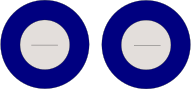
\includegraphics[width=0.5\textwidth]{images/intro/images/rings/rings}
%   \caption{Bodies under collision which are divided into primary and
%     secondary.}
% \label{fig:bodies_under_collision}
% \end{figure}

% Two different Poisson ratios are simulated. \Cref{fig:rings:sun2019-nu-0.3975}
% shows the particle positions of rings with a Poisson ratio of $0.3975$ when
% simulated with SPST. The recovery of the colliding rings without any tensile
% instability can be seen.

% We also consider higher Poisson ratios, such as 0.47.
% \Cref{fig:rings:sun2019-nu-0-47} shows the particle positions of rings when
% simulated with SPST and \cref{fig:rings:ipst-nu-0-47} with IPST. Even though
% both the particle shifting techniques are able to eliminate the numerical
% fracture, IPST gives better results as in the distribution of particles
% through out the simulation, see \cref{fig:rings:sun2019-nu-0.47-2} and
% \cref{fig:rings:ipst-nu-0.47-2}. For the case where SPST is used, the final
% particle distribution is not very uniform. This is not the case when IPST is
% used. We can therefore say that IPST performs better than SPST.
% %
% \begin{figure}
%   \centering
%   \begin{subfigure}{0.48\textwidth}
%     \centering
%     \includegraphics[width=1.0\textwidth]{figures/intro/figures/rings/time0}
%     \subcaption{t = 0 sec}\label{fig:rings:sun2019-nu-0.3975-0}
%   \end{subfigure}
%   %
%   \begin{subfigure}{0.48\textwidth}
%     \centering
%     \includegraphics[width=1.0\textwidth]{figures/intro/figures/rings/time1}
%     \subcaption{t = 2.5e-03 sec}\label{fig:rings:sun2019-nu-0.3975-1}
%   \end{subfigure}
% % %
% %   \begin{subfigure}{0.48\textwidth}
% %     \centering
% %     \includegraphics[width=1.0\textwidth]{figures/intro/figures/rings/time2}
% %     \subcaption{t = 4e-03 sec}\label{fig:rings:sun2019-nu-0.3975-2}
% %   \end{subfigure}

%   \begin{subfigure}{0.48\textwidth}
%     \centering
%     \includegraphics[width=1.0\textwidth]{figures/intro/figures/rings/time3}
%     \subcaption{t = 7.3e-03 sec}\label{fig:rings:sun2019-nu-0.3975-3}
%   \end{subfigure}
% %
%   \begin{subfigure}{0.48\textwidth}
%     \centering
%     \includegraphics[width=1.0\textwidth]{figures/intro/figures/rings/time4}
%     \subcaption{t = 1.45e-02 sec}\label{fig:rings:sun2019-nu-0.3975-4}
%   \end{subfigure}
% % %
% %   \begin{subfigure}{0.3\textwidth}
% %     \centering
% %     \includegraphics[width=1.0\textwidth]{figures/intro/figures/rings/time5}
% %     \subcaption{t = 1.5e-02 sec}\label{fig:rings:sun2019-nu-0.3975-5}
% %   \end{subfigure}
%   \caption{Rings with a Poisson ratio of 0.3975 colliding head on, simulated with CTVF using SPST.}
% \label{fig:rings:sun2019-nu-0.3975}
% \end{figure}
% %


\section{Summary}
We gave an overview of modeling the abrasive water jet machining. After
reviewing the possible techniques to simulate it through mesh-based schemes and
meshless methods, due to the computational limits and ease of modeling, we chose
meshless methods. Among many meshless methods, we have chosen the SPH method in
the current work, and this is due to the developed software available in the
group and work done in literature on SPH history. At the same time, DEM is used
to model the interaction between the rigid bodies. An outline of the current
thesis is set. We start with the present chapter to handle the fluid and elastic
dynamics.

In the current chapter, among all the required physics to be simulated, we have
chosen to handle the fluid and elastic dynamics. In the such process we
introduced the equations governing the fluid and structural dynamics. We
introduced the basic SPH equations and how SPH approximates functions and
derivatives. SPH is applied to solve the fluid and elastic dynamics, through
which better SPH approximations are discussed. We found that the SPH without any
corrections has several issues, like tensile instability, and inhomogeneous
particle distribution leading to poorer accuracy of the simulation. SPH has
accuracy issues, and it cannot produce 2nd order accurate results.

In the next chapter, we will propose a particle shifting technique into SPH and
move the particles with transport velocity rather than momentum velocity. And
check solve the particle homogenization problems, tensile instability. Problems
involving boundaries are handled as well.

%  We gave an overview of modeling the abrasive water jet machining. After
% reviewing the possible techniques to simulate it through mesh-based schemes and
% meshless methods, due to the computational limits and ease of modeling, we chose
% meshless methods. Among many meshless methods, we have chosen the SPH method to
% model the fluid and elastic dynamics in the current work. At the same time, DEM
% is used to model the interaction between the rigid projectiles.

%  In the current chapter, we introduce the basics of smoothed particle
% hydrodynamics. We have discussed the function, derivative and divergence
% approximations in SPH. In the next chapter, we will develop a scheme where a
% particle shifting technique into SPH and apply it to solve

\include{chapter_ctvf/ctvf}
\chapter{Collision SPH}
\label{chap:csph}



\section{Introduction}
\label{sec:intro}
In the current chapter we model the collision between elastic bodies. Modeling
the collision among elastic solids allows us to handle the interaction between
the target and the impactor when they are assumed as elastic or elastic-plastic.
An SPH based solution leads to unphysical interactions in modeling the collision
of objects when they are close by but not touching. Further, SPH model does not
incorporate friction between the colliding bodies. In the current chapter, a
contact force model is incorporated into the existing solver to handle the
interaction between the colliding solids. Specifically, we consider bodies with
arbitrary shapes.


The collision of arbitrary solid bodies occurs everywhere around us. Apart
from the elastic collision of bodies, other important examples include surface
erosion, waterjet machining \citep{natarajan2020abrasive}, and machining
processes \citep{islam2020numerical} to note a few. It is important to be able
to simulate such problems accurately.

% When body A discretized into n particles is colliding a body B which is
% discretized in to m particles, above techniques use the particles in B to
% compute the accelerations of density and velocity of particles in A. A few
% drawbacks of this approach is, the bodies come in to contact even when the
% bodies are physically not touching, and the no frictional modeling is modeled.
% \cite{yan2021simulation} has proposed a interfacial SPH scheme , where each
% elastic body uses their own particles in computation of divergence, momentum
% and strain rate. While, the bodies interact by a repulsive force inspired from
% Ansys. Where they have shown the improvement on modeling the collision with
% different examples. Yan has considered Gray SPH which is not so great with
% kernel invariance as it shows tensile instability with a few kernels as shown
% by Roth 2020. Also the contact force model didn't incorporate the frictional
% part of the collision. Further the contact force has a influence of 2h radius,
% implies there would be a force acting on the interacting bodies though they
% are not touching physically.

% The contact force model used in Yan is inspired from ANSYS model and is given.
% A similar work is done by \cite{vyas2021collisional}, where the author models
% the interaction between a circular rigid body impacting a target surface. In
% his work, author proposes a non-linear penalty based force model which could
% handle friction as well and studies the rebounding characteristic of the
% impactor. Here, the author studies the post collision behaviour of the
% circular rigid body which is interacting the elastic plastic solid at
% different incident angles. \cite{mohseni2021particle} proposed an advanced
% version of the collision model where he models the interaction between a rigid
% body with a brittle solids and models the erosion of the brittle solid.

% Finally the current model comes into place only when the material interfaces
% are touching unlike what Yan's contact force model and conventional SPH. We
% also check the invariance of the current scheme in modeling the collisions for
% different types of kernels used.


In the current work, the collision between elastic solids is modeled using a
penalty-based contact force model. A contact force based approach for collision
handling will eliminate the spurious interaction between bodies, which occurs
while modeling with an SPH-based model. Unlike the approach of
\citep{yan2021simulation}, the proposed contact force model can handle friction
between the solids as well. The bodies themselves are elastic and this is
simulated using the CTVF SPH method \citep{adepu2021corrected}. The
penalty-based force considered here is the one proposed by
\cite{mohseni2021particle}. In the original model proposed by
\citep{mohseni2021particle}, the contact force is between a primary body and a
secondary body. In \citep{mohseni2021particle}, the primary body is usually
treated as the rigid body and the body on which the erosion is simulated is
treated as secondary. It is not clear what would happen if both bodies were
elastic or if there is no clear way to distinguish between a primary and
secondary body. We explore these questions in the present work. The work of
\cite{mohseni2021particle} takes inspiration from that of
\cite{vyas2021collisional} where too there is a clear distinction between
primary and secondary bodies. \cite{vyas2021collisional} also consider the
collision between a rigid and elastic body. In the present work we only
implement the collision model of \citep{mohseni2021particle} due to its
simplicity. The model proposed by \cite{vyas2021collisional} is more complex to
implement. Several examples are simulated to validate the current scheme,
ranging from simulations compared with FEM, analytical results as well as
experimental. We next look at the numerical method used to model the collision
among the elastic solids.


\FloatBarrier%
\section{SPH model for structural dynamics}
\label{sec:SPH-model-for-structural-dynamics}

\subsection{Discrete governing equations}
\label{sec:discrete-governing-equations}
We follow the CTVF formulation developed in \cref{chap:ctvf} to handle the
structural dynamics of the solid. The governing equations of including the new
contact force term are:
\begin{equation}
\label{eqn:sph-continuity}
  \frac{\tilde{d}\rho_a}{dt} = \sum_{b \in A} \; \frac{m_b}{\rho_{b}} \; (
  \rho_{a} \; \tilde{\ten{u}}_{ab} \; + \;
  (\rho \; (\tilde{\ten{u}} \; - \;
  \ten{u}))_{ab}) \; \cdot \nabla_{a} W_{ab},
\end{equation}
\begin{equation}
\label{eqn:sph-momentum}
  \frac{\tilde{d}\ten{u}_{a}}{dt} = - \sum_{b \in A} m_b \bigg[
  \bigg(\frac{p_a}{\rho_a^2} + \frac{p_b}{\rho_b^2}\bigg) \ten{I} -
  \bigg(\frac{\teng{\sigma}^{'}_{a}}{\rho_a^2} +
  \frac{\teng{\sigma}^{'}_{b}}{\rho_b^2} + \Pi_{ab} \ten{I} \bigg) \bigg]  \cdot \nabla_{a} W_{ab} +
  \ten{g}_{a} + \frac{1}{m_a}\sum_{b \in B} \ten{F}^{\text{cont}}_{a \leftarrow b}.
\end{equation}
Here, $\ten{F}^{cont}_{a}$ is the force acting on particle $a$ due to
\begin{figure}[!htpb]
  \centering
  \includegraphics[width=1.0\textwidth]{images/csph/images/contact_force/contact_force_description}
  \caption{Bodies under collision which are divided into primary and
    secondary.}
\label{fig:bodies_under_collision}
\end{figure}
contact with the other elastic bodies which will be discussed in
\cref{sec:contact-algorithm}. We follow \cref{chap:ctvf} in handling the
boundaries , in updating the state of the bodies to the next stage, while
transporting particles with a PST.


\FloatBarrier%
\section{Contact algorithm}
\label{sec:contact-algorithm}
In the current work we have utilized the contact force model proposed by
\cite{mohseni2021particle}. The force acting on a particle $a$ of body A due
to the interaction with the particles of body $B$ can be resolved into a
normal and tangential component. The normal force component is utilised to
make sure that the particles of different bodies do not penetrate into each
other, while the tangential component is used to model the friction between
the interacting solids. According to \cite{mohseni2021particle}, we divide the
bodies under interaction into primary and secondary bodies, as shown in
\cref{fig:bodies_under_collision}.
% In usual DEM to compute the force on particle i of body A, the force is
% computed by considering the overlap of particle i with each and every
% particle of body j by considering the particle j to be spherical. This leads
% to unphysical modeling of contact force when the body is interacting with a
% flat surface or surfaces which are not spherical by nature. The current
% contact force is surface aware. The force on particle $i$ is computed by
% equation
The normal force ($\teng{F}_a^{n}$) on
particle $a$ due to the interaction with the particles $b$ of body $B$ is
computed as,
\begin{equation}
  \label{eq:contact-algorithm-normal}
  \ten{F}_a^n = k_r \delta_{n^{c}}^{a} \ten{n}_a^{c}.
\end{equation}
Here, the overlap $\delta_{n^{c}}^{a}$ is computed using
\begin{equation}
  \label{eq:csph:cf-overlap}
  \delta_{n^{c}}^{a} = \Delta x - d_a,
\end{equation}
where,
\begin{equation}
  \label{eq:cf-distance-computation}
  d_a = \frac{
    \displaystyle\sum\limits_{b = 1}^{\text{NP}^{b}} \;
    \big( \ten{n}_a^{c} \cdot \ten{r}_{ab} \big)  \frac{m_b}{\rho_b} W_{ab}}
  {
    \displaystyle\sum\limits_{b = 1}^{\text{NP}^{b}} \;
    \frac{m_b}{\rho_b} W_{ab}},
\end{equation}
and the normal contact vector $\ten{n}_a^{c}$ is computed using
\begin{equation}
  \label{eq:cf-normal-vector}
  \ten{\hat{n}}_a^{c} = \frac{
    \displaystyle\sum\limits_{b = 1}^{\text{NP}^{b}} \;
    \frac{\ten{r}_{ab}}{r_{ab}}  \frac{m_b}{\rho_b} W_{ab}}
  {
    \displaystyle\sum\limits_{b = 1}^{\text{NP}^{b}} \;
    \frac{m_b}{\rho_b} W_{ab}},
\end{equation}
\begin{equation}
  \label{eq:cf-normal-vector}
  \ten{n}_a^{c} = \frac{\teng{\hat{n}}_a^{c}}{||\teng{\hat{n}}_a^{c}||}.
\end{equation}
\begin{figure}[!htpb]
  \centering
  \includegraphics[width=0.3\textwidth]{images/csph/images/contact_force/contact_force_delta_computation}
  \caption{Pictorial representation of distance between a particle and a body.}
\label{fig:contact_force_delta_computation}
\end{figure}
Where $\Delta x$ being the initial spacing between the particles, $k_r$ is the
normal spring stiffness coefficient. \Cref{fig:contact_force_delta_computation}
shows $\Delta x$ and $d_a$ quantities, respectively. Note that while computing
the overlap of particle $a$ with the body $B$ we have computed an effective
overlap, rather than per particle interaction. This is effectively able to model
the interaction between non-smooth surfaces in contrast with particle-particle
force computation.

\subsection{Tangential force computation}
\label{sec:tangential-force-computation}
We associate a tangential spring attached to particle $a$
($|\Delta \textit{\textbf{l}}_a|$) and body $B$ to compute the tangential force
($\ten{F}_{a}^{t}$), which initially has a magnitude of zero
($|\Delta \textit{\textbf{l}}_a|=0$). The tangential spring is activated when
the particle comes into contact with body $B$. The tangential force is
history-dependent. The contact friction force is proportional to the tangential
spring displacement, which is integrated over the contact time as
\begin{equation}
  \label{eq:tangential-force}
  \ten{F}_{a}^{t^{n+1}} =
  -k_f \Delta \textit{\textbf{l}}_a^{\,n + 1} =
  -k_f \big[\big(\Delta {\textit{\textbf{l}}}_a^{\,n} \
  + \ten{v}_{ab}^{n + 1} \Delta t\big) \cdot \ten{t}_a^{n + 1} \big] \
  \ten{t}_a^{n + 1},
\end{equation}
where $\Delta t$ is the time step, $\ten{v}_{ab} = \ten{v}_{a} - \ten{v}_b$ is
the relative velocity of the primary particle $a$ with respect to the closest
secondary particle $b$, $\ten{t}_a$ is the tangential unit vector, and $k_f$ is the tangential spring stiffness
coefficient. Here, $n$ and $n+1$ represent the times which are $\Delta t$ apart.
The tangential unit vector is computed by,
\begin{equation}
  \label{eq:tangential-vect}
  \ten{t}_a = \frac{\ten{v}_{ab} - (\ten{v}_{ab} \cdot \ten{n}_a^{c}) \ten{n}_a^{c}}{|\ten{v}_{ab} - (\ten{v}_{ab} \cdot \ten{n}_a^{c}) \ten{n}_a^{c}|}.
\end{equation}

The tangential force is coupled to the normal force through the Coulomb's law,
\begin{equation}
  \label{eq:Coulomb-law}
  \ten{F}_{a}^{t} = \min(\mu |\ten{F}_{a}^{n}|, |\ten{F}_{a}^{t}|) \
  \frac{\ten{F}_{a}^{t}}{|\ten{F}_{a}^{t}|}.
\end{equation}
This allows us to impose the sliding friction condition between the
interacting solids. Finally, the total force acting on the particle $a$ due to
the interaction with body $B$ is:
\begin{equation}
  \label{eq:contact-force}
  \ten{F}_{a}^{\text{cont}} = \ten{F}_{a}^{n} + \ten{F}_{a}^{t}
\end{equation}

\begin{figure}[!htpb]
  \centering
  \includegraphics[width=0.3\textwidth]{images/csph/images/contact_force/contact_force_description_3}
  \caption{Force transfer to the secondary particles $b$ from the primary body particle $a$}
\label{fig:secondary_particle_contact_foce_transfer}
\end{figure}
An equal and opposite force of the same magnitude is applied to the closest
secondary particle $b$ of $a$ as shown in
\cref{fig:secondary_particle_contact_foce_transfer},
\begin{equation}
  \label{eq:contact-force}
  \ten{F}_{b}^{\text{cont}} = - \ten{F}_{a}^{\text{cont}}.
\end{equation}

% The force on the particle $j$ is evaluated, on the
% body belonging to the secondary surface is as follows. Particles belonging to
% the secondary surface ($j$) which are at a distance less than the initial
% spacing ($l_0$) share the force exerted on particle i, as following:
% \begin{equation}
%   \label{eq:cf-overlap}
%   F^{ij} = - F^{i} w^{ij},
% \end{equation}
% where $w^{ij}$ is defined as
% \begin{equation}
%   \label{eq:cf-overlap}
%   w^{ij} = \frac{n^{i} \cdot \hat{\ten{r}}^{ij}}{\sum_j n^{i} \cdot \hat{\ten{r}}^{ij}}
% \end{equation}

The current contact force model is sensitive towards the primary body chosen
to compute the forces, i.e., the force acting on the particles is not the same
when the primary bodies are interchanged. In the current work we have explored
the behaviour of the current contact force model when different bodies are
chosen as primary and secondary. Simulations such as, a rectangular solid
sliding down an inclined plane, and a symmetric collision between elastic
solids are two examples, where we have investigated how the bodies would behave
when different bodies are chosen as primary.
% , as shown in \cref{fig:primary-secondary-demonstration}.
% \begin{figure}[!htpb]
%   \centering
%   \begin{subfigure}{0.48\textwidth}
%     \centering
%     \includegraphics[width=1.0\textwidth]{images/csph/images/primary_vs_secondary/sliding}
%     \subcaption{A sliding body.}%\label{fig:rings:ipst-nu-0.47-0}
%   \end{subfigure}
%   \begin{subfigure}{0.48\textwidth}
%     \centering
%     \includegraphics[width=1.0\textwidth]{images/csph/images/primary_vs_secondary/symmetric_collision}
%     \subcaption{A symmetric collision between rectangular solids.}%\label{fig:rings:ipst-nu-0.47-1}
%   \end{subfigure}
%   \caption{Examples used to explore the importance of choosing a primary.}
% \label{fig:primary-secondary-demonstration}
% \end{figure}

% =========================================== %
% ------ Results start ---------------------- %
% =========================================== %

\FloatBarrier%
\section{Results and discussion}
\label{sec:results}
In the interest of reproducibility and easier ability
for researchers to build on this work, our code is open source and can be
found at \url{https://gitlab.com/pypr/collision_sph}. We use the
\texttt{automan} package~\citep{automan2018} to automate all the results
generated.

\FloatBarrier%
\subsection{Curved interface}
\label{sec:results-circular-interface}
\begin{figure}[!htpb]
  \centering
  \includegraphics[width=0.6\textwidth]{images/csph/images/yan_2021_curved_interface/schematic}
  \caption{Collision between two circular elastic discs. The left disc moves
    towards the right disc with a constant velocity $v_0$, while the right
    disc is at rest.}
\label{fig:results-yan-circular-interface-schematic}
\end{figure}
The collision of two circular elastic solids is considered as the first test
case. \Cref{fig:results-yan-circular-interface-schematic} shows the initial
configuration where the left disc is initially allowed to move towards the
right with a velocity of 20 m\,s\textsuperscript{-1}. While no velocity is
imposed on the right disc. The radius of each disk is $0.4$ m, and made of
Aluminium, whose material properties are shown in
\cref{tab:curved-interface-material-params}. No friction and gravity is
assumed in the current case. A particle spacing of 0.01 m is used, resulting
in a $4779$ particles per disc. The numerical parameters utilized in
the current example are shown in \cref{tab:curved-interface-numerical-params}.
\begin{table}[!ht]
  \centering
  \begin{tabular}[!ht]{ll}
    \toprule
    Quantity & Values\\
    \midrule
    $E$, Young's modulus & $72$ GPa \\
    $\nu$, Poisson's ratio & $0.3$ \\
    $\rho$, density & $2785$ kg\,m\textsuperscript{-3} \\
    $\mu$, friction coefficient & $0$ \\
    Time of simulation & $4$ ms \\
    gravity $[g_x, g_y, g_z]$ & $[0.0, 0.0, 0.0]$\\
    \bottomrule
  \end{tabular}
  \caption{Material parameters used for the impact of curved interface problem.}%
  \label{tab:curved-interface-material-params}
\end{table}
\begin{table}[!ht]
  \centering
  \begin{tabular}[!ht]{ll}
    \toprule
    Quantity & Values\\
    \midrule
    $\delta x $, Resolution & $0.01$\\
    $h/\Delta x$, Smoothing length factor & 1\\
    $\alpha$, artificial viscosity & $1$ \\
    $\beta$, artificial viscosity & $0$ \\
    $k_r$, Normal stiffness coefficient & $10^{10}$ \\
    $k_f$, Tangential stiffness coefficient & $10^{9}$ \\
    \bottomrule
  \end{tabular}
  \caption{Numerical parameters used for the impact of curved interface problem.}%
  \label{tab:curved-interface-numerical-params}
\end{table}

\Cref{fig:yan-2021-curved:improved-ipst-nu-0-47} shows the snapshots of
particles of the circular disc under contact by the present approach including
the stress ($\sigma_{xx}$) field at times $t=0.0, 1.8, 4$ ms. From the figure,
we can see that the current numerical scheme is able to reproduce smooth
stress fields. The elastic discs are initially in stress free state, and once
the bodies collide, the left disc transfers its momentum to the right. Since
the discs are elastic, the total momentum is not transferred, and the left
disc will not come to a halt but rather starts moving with the free vibration
of the disc.
\begin{figure}[!htpb]
  \centering
  \begin{subfigure}{0.48\textwidth}
    \centering
    \includegraphics[width=1.0\textwidth]{figures/csph/figures/yan_2021_curved_interface/collision_ctvf/time0}
    \subcaption{t = $0$ ms}\label{fig:rings:ipst-nu-0.47-0}
  \end{subfigure}
  \begin{subfigure}{0.48\textwidth}
    \centering
    \includegraphics[width=1.0\textwidth]{figures/csph/figures/yan_2021_curved_interface/collision_ctvf/time1}
    \subcaption{t = $1.8$ ms}\label{fig:rings:ipst-nu-0.47-1}
  \end{subfigure}

  \begin{subfigure}{0.48\textwidth}
    \centering
    \includegraphics[width=1.0\textwidth]{figures/csph/figures/yan_2021_curved_interface/collision_ctvf/time2}
    \subcaption{t = $4$ ms}\label{fig:rings:ipst-nu-0.47-2}
  \end{subfigure}
  \caption{The stress field of the elastic discs at three different time
    instants through the collision.}
\label{fig:yan-2021-curved:improved-ipst-nu-0-47}
\end{figure}

\Cref{fig:results-yan-curved-velocity-vs-time} presents the time histories of
the velocity of the center of mass of both the discs in comparison with the
results by FEM solver presented in \citep{yan2021simulation}. The rebound the
velocity of the bodies with the current scheme is in good match with the FEM
result.
% \todoin{Add why CTVF is different}
\begin{figure}[!htpb]
  \centering
  \includegraphics[width=0.6\textwidth]{figures/csph/figures/yan_2021_curved_interface/velocity_vs_time}
  \caption{Time history of the x component of velocity of center of mass's of
    the left and the right disc, and compared with the numerical results
    produced using FEM, CTVF. The Young's modulus of the disc is taken as
    $E$=$72$ GPa.}
\label{fig:results-yan-curved-velocity-vs-time}
\end{figure}

We check if the elastic disk behave as a rigid disk with an increase in
Young's modulus and is able to retrieve the rigid velocity. We expect the
right disk to achieve the velocity of $20$ m\,s\textsuperscript{-1} as the
Young's modulus is increased. \Cref{fig:results-yan-curved-E-vs-velocity}
shows the variation of the final velocity of the right disc with Young's
modulus, where we can see that the proposed model is behaving as expected.
\begin{figure}[!htpb]
  \centering
  \includegraphics[width=0.6\textwidth]{figures/csph/figures/yan_2021_curved_interface/E_vs_velocity}
  \caption{Variation of the x-velocity of the center of mass with Young's
    modulus of the disc.}
\label{fig:results-yan-curved-E-vs-velocity}
\end{figure}

% ===================================================
% ===================================================
\FloatBarrier%
\subsection{Flat interface}
\label{sec:results-linear-interface}
In the current section, we test our solver in handling collision between two
elastic solids, where the collision front is flat in shape. The model is
shown in \cref{fig:results-yan-linear-interface-schematic}. Both the solids
are of the same size, $0.2$ m in length and $0.1$ m in height. The material is
the same as in the circular interface problem
(\cref{sec:results-circular-interface}) and can be found in
\cref{tab:curved-interface-material-params}, while the numerical parameters
are listed in \cref{tab:linear-interface-numerical-params}. A particle spacing
of $0.0025$ m is used, resulting in $3321$ particles per body.
\begin{figure}[!htpb]
  \centering
  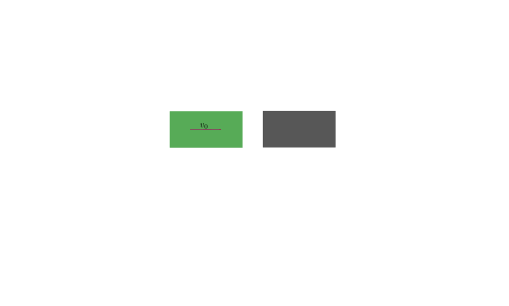
\includegraphics[width=0.8\textwidth]{images/csph/images/yan_2021_linear_interface/schematic}
  \caption{
    Collision between two rectangular elastic solids, where, the left solid is allowed
    to move towards the right solid with a constant velocity $v_0$, while the right
    solid is at rest.}
\label{fig:results-yan-linear-interface-schematic}
\end{figure}
\begin{table}[!ht]
  \centering
  \begin{tabular}[!ht]{ll}
    \toprule
    Quantity & Values\\
    \midrule
    $h/\Delta x$, Smoothing length factor & 1\\
    $\alpha$, artificial viscosity & $1$ \\
    $\beta$, artificial viscosity & $0$ \\
    $k_r$, Normal stiffness coefficient & $10^{11}$ \\
    $k_f$, Tangential stiffness coefficient & $10^{9}$ \\
    \bottomrule
  \end{tabular}
  \caption{Numerical parameters used for the impact of linear interface problem.}%
  \label{tab:linear-interface-numerical-params}
\end{table}

\Cref{fig:results-yan-linear-velocity-vs-time} shows the velocity of the
center of mass of both the bodies using current scheme along with the
formulation of \cite{gray2001sph} and with FEM results provided by
\cite{yan2021simulation}. From the
\cref{fig:results-yan-linear-velocity-vs-time} we can see that rebound
velocities match well with the FEM results provided, as well as the
interaction between the bodies start when their physical boundaries have come
into contact, in contrast to SPH, where the bodies interact when the other
body is in its smoothing length influence. The rebound velocity of the current
scheme is matches well with FEM result. Since the body is elastic,
after the collision, both the bodies move with the base oscillation amplitude
% \todoin{Try to explain oscillation amplitude}
which is the reason why the left body does not achieve a zero velocity.
The current scheme results are better than the CTVF model.
\begin{figure}[!htpb]
  \centering
  \includegraphics[width=0.6\textwidth]{figures/csph/figures/yan_2021_linear_interface/velocity_vs_time}
  \caption{Time history of the x component of the center of mass's velocity of
    the left and the right rectangular bodies, and compared with the numerical
    results produced using FEM, SPH.}
\label{fig:results-yan-linear-velocity-vs-time}
\end{figure}


\FloatBarrier%
\subsection{Colliding rubber rings}
\label{sec:results-rings}
This test applies the current solver in modeling large deformation solids
under collision. We consider the collision between two elastic rubber rings.
This benchmark is simulated by various works in SPH literature, such as in
\cite{gray2001sph,adepu2021corrected,zhang2017generalized}.

\begin{figure}[!htpb]
  \centering
  \includegraphics[width=0.7\textwidth]{images/csph/images/yan_2021_colliding_rubber_rings/schematic}
  \caption{Schematic sketch of the initial setup of colliding rubber rings.}
\label{fig:colliding_rings}
\end{figure}
The initial positioning, as well as the dimensions of the rings, are shown in
\cref{fig:colliding_rings}. Both rings are made of the same material, whose
material properties are listed in \cref{tab:colliding-rings-material-params},
and the numerical parameters in \cref{tab:colliding-rings-numerical-params},
respectively. The initial relative velocity at which the rings collide is
$v_0 = 0.12 c_0$ m\,s\textsuperscript{-1}.

\begin{table}[!ht]
  \centering
  \begin{tabular}[!ht]{ll}
    \toprule
    Quantity & Values\\
    \midrule
    $E$, Young's modulus & $10$ MPa \\
    $\nu$, Poisson's ratio & $0.47$ \\
    $\rho$, density & $1200$ kg\,m\textsuperscript{-3} \\
    $\mu$, friction coefficient & $0.0$ \\
    Time of simulation & $0.016$ s \\
    Resolution, $\delta x$ & $0.001$ m\\
    Smoothing length factor, $h/\Delta x$ & 1.3\\
    gravity $[g_x, g_y, g_z]$ & $[0.0, 0.0, 0.0]$\\
    \bottomrule
  \end{tabular}
  \caption{Material parameters used for modeling the impact of elastic rubber rings.}%
  \label{tab:colliding-rings-material-params}
\end{table}

\begin{table}[!ht]
  \centering
  \begin{tabular}[!ht]{ll}
    \toprule
    Quantity & Values\\
    \midrule
    $\alpha$, artificial viscosity & $1$ \\
    $\beta$, artificial viscosity & $0$ \\
    $k_r$, Normal stiffness coefficient & $10^{7}$ \\
    $k_f$, Tangential stiffness coefficient & $10^{5}$ \\
    \bottomrule
  \end{tabular}
  \caption{Numerical parameters used for modeling the impact of elastic rubber rings.}%
  \label{tab:colliding-rings-numerical-params}
\end{table}

The evolution of the rings is shown in \cref{fig:rings:new-ipst-nu-0-47}, we
can see from the figure that the current model has reproduced a stable and
smooth stress field. The rings are stress free before the collision, as shown
in \cref{fig:rings:ipst-nu-0.47-1}. Throughout the simulation phase, while the
rings are colliding, the kinetic energy of the rings is transferred into
elastic and vice versa. At the maximum deformation, the elastic energy stored
in the rings is maximum. After that, both the rings bounce off and start to
separate. Further, we can see the rings being under tension as well as
compression, while it is deforming in \cref{fig:rings:ipst-nu-0.47-3}. The
results are consistent with other numerical methods proposed by
\cite{gray2001sph} and \cite{zhang2017generalized}.
\begin{figure}[!htpb]
  \centering
  \begin{subfigure}{0.48\textwidth}
    \centering
    \includegraphics[width=1.0\textwidth]{figures/csph/figures/yan_2021_colliding_rubber_rings/poisson_ratio_0_47/time0}
    \subcaption{t = $0$ ms}\label{fig:rings:ipst-nu-0.47-1}
  \end{subfigure}
  %
  \begin{subfigure}{0.48\textwidth}
    \centering
    \includegraphics[width=1.0\textwidth]{figures/csph/figures/yan_2021_colliding_rubber_rings/poisson_ratio_0_47/time1}
    \subcaption{t = $1.38$ ms}\label{fig:rings:ipst-nu-0.47-2}
  \end{subfigure}

  \begin{subfigure}{0.48\textwidth}
    \centering
    \includegraphics[width=1.0\textwidth]{figures/csph/figures/yan_2021_colliding_rubber_rings/poisson_ratio_0_47/time2}
    \subcaption{t = $5.17$ ms}\label{fig:rings:ipst-nu-0.47-3}
  \end{subfigure}
%
  \begin{subfigure}{0.48\textwidth}
    \centering
    \includegraphics[width=1.0\textwidth]{figures/csph/figures/yan_2021_colliding_rubber_rings/poisson_ratio_0_47/time3}
    \subcaption{t = $7.38$ ms}\label{fig:rings:ipst-nu-0.47-4}
  \end{subfigure}

  \begin{subfigure}{0.48\textwidth}
    \centering
    \includegraphics[width=1.0\textwidth]{figures/csph/figures/yan_2021_colliding_rubber_rings/poisson_ratio_0_47/time4}
    \subcaption{t = $11.462$ ms}\label{fig:rings:ipst-nu-0.47-3}
  \end{subfigure}
%
  \begin{subfigure}{0.48\textwidth}
    \centering
    \includegraphics[width=1.0\textwidth]{figures/csph/figures/yan_2021_colliding_rubber_rings/poisson_ratio_0_47/time5}
    \subcaption{t = $15.4$ ms}\label{fig:rings:ipst-nu-0.47-4}
  \end{subfigure}
  \caption{Snapshots of particle positions with color indicating the stress
    field ($\sigma_{xx}$) solved by the current solver.}
\label{fig:rings:new-ipst-nu-0-47}
\end{figure}
%

% ====================================================================================
% ====================================================================================
\FloatBarrier%
\subsection{Near miss of two solids}
\label{sec:results-two-solids-passing-by}
In this section, we study the collision behavior of two solids moving toward
each other, initially placed such that they are not touching. The schematic is
shown in \cref{fig:results-solid-passing-by-schematic}. We show that the current
model is able to eliminate the unphysical interaction that arises due to the
conventional SPH, which is due to the physical influence of the particles at the
boundary. We expect no change in the velocity of the elastic solids as they pass
by. We show that with the current model no interaction exists when the elastic
solids are physically not touching, and no variation in their path is found. As
a qualitative validation the particle plots is shown and for quantitative
validation, variation of the velocity of the center of mass of the elastic body
with time is considered.

\begin{figure}[!htpb]
  \centering
  \includegraphics[width=0.7\textwidth]{images/csph/images/dinesh_2022_elastic_solids_passing_by/schematic}
  \caption{Schematic of the two elastic solids which are placed close to each
    other and allowed to move at a constant velocity $v_0$ with opposite signs.}
\label{fig:results-solid-passing-by-schematic}
\end{figure}
The dimensions of the elastic bodies under consideration are as follows, the
length and height are $0.2$ m and $0.1$ m, respectively. Both bodies are made
of density $1200$ kg\,m\textsuperscript{-3}, Young��s modulus of $10$ MPa and
Poisson��s ratio of $0.4$. The left body is allowed to
move to the right in the x-direction with a velocity of $v_0=20$
m\,s\textsuperscript{-1}, and the right body with $v_0=-20$
m\,s\textsuperscript{-1}. A particle spacing of dx $=0.0025$ m is used, which
results in 3321 particles per single body. We have turned off the particle
shifting in the current test case as no deformation of the bodies is expected.

\begin{figure}[!htpb]
  \centering
  \begin{subfigure}{0.48\textwidth}
    \centering
    \includegraphics[width=1.0\textwidth]{figures/csph/figures/dinesh_2022_elastic_solids_passing_by/CTVF/time0}
    \subcaption{t = $0$ ms}\label{fig:passing-0}
  \end{subfigure}
  %
  \begin{subfigure}{0.48\textwidth}
    \centering
    \includegraphics[width=1.0\textwidth]{figures/csph/figures/dinesh_2022_elastic_solids_passing_by/CTVF/time1}
    \subcaption{t = $1.4$ ms}\label{fig:passing-1}
  \end{subfigure}

  \begin{subfigure}{0.48\textwidth}
    \centering
    \includegraphics[width=1.0\textwidth]{figures/csph/figures/dinesh_2022_elastic_solids_passing_by/CTVF/time2}
    \subcaption{t = $10$ ms}\label{fig:passing-2}
  \end{subfigure}
  %
  \begin{subfigure}{0.48\textwidth}
    \centering
    \includegraphics[width=1.0\textwidth]{figures/csph/figures/dinesh_2022_elastic_solids_passing_by/CTVF/time3}
    \subcaption{t = $12$ ms}\label{fig:passing-3}
  \end{subfigure}
  \caption{Snapshots of the bodies passing close by when simulated with CTVF.}
  \label{fig:dinesh-2022-passing-ctvf}
\end{figure}
%

\begin{figure}[!htpb]
  \centering
  \begin{subfigure}{0.48\textwidth}
    \centering
    \includegraphics[width=1.0\textwidth]{figures/csph/figures/dinesh_2022_elastic_solids_passing_by/Mohseni_Vyas/time0}
    \subcaption{t = $0$ ms}\label{fig:passing-0}
  \end{subfigure}
  %
  \begin{subfigure}{0.48\textwidth}
    \centering
    \includegraphics[width=1.0\textwidth]{figures/csph/figures/dinesh_2022_elastic_solids_passing_by/Mohseni_Vyas/time1}
    \subcaption{t = $1.4$ ms}\label{fig:passing-1}
  \end{subfigure}

  \begin{subfigure}{0.48\textwidth}
    \centering
    \includegraphics[width=1.0\textwidth]{figures/csph/figures/dinesh_2022_elastic_solids_passing_by/Mohseni_Vyas/time2}
    \subcaption{t = $10$ ms}\label{fig:passing-2}
  \end{subfigure}
  %
  \begin{subfigure}{0.48\textwidth}
    \centering
    \includegraphics[width=1.0\textwidth]{figures/csph/figures/dinesh_2022_elastic_solids_passing_by/Mohseni_Vyas/time3}
    \subcaption{t = $12$ ms}\label{fig:passing-3}
  \end{subfigure}
  \caption{Snapshots of the bodies passing close by when simulated with current solver.}
\label{fig:dinesh-2022-passing-collision}
\end{figure}
%
\Cref{fig:dinesh-2022-passing-ctvf} shows the snapshots of bodies at multiple
time instants simulated using the formulation of \cite{adepu2021corrected}.
From \Cref{fig:dinesh-2022-passing-ctvf} we can see that the bodies interact
with each other though they are not touching physically, this is because in
SPH the particles at the boundaries have an influence radius exceeding its
material boundary. Because of the interaction, shear stresses develop, which
results in strain in the body as well as it deviates from its path.
\Cref{fig:dinesh-2022-passing-collision} shows the snapshots of bodies when
simulated with the current contact force model with the current SPH
formulation. From \cref{fig:dinesh-2022-passing-collision}, we can clearly see
that the bodies don't interact and pass freely without any deformations or
path divergence.
\begin{figure}[!htpb]
  \centering
  \includegraphics[width=0.48\textwidth]{figures/csph/figures/dinesh_2022_elastic_solids_passing_by/velocity_vs_time_x}
  \includegraphics[width=0.48\textwidth]{figures/csph/figures/dinesh_2022_elastic_solids_passing_by/velocity_vs_time_y}
  \caption{Time variation of the x-component and y-component of the velocity
    of the center of mass of the freely moving rectangular solids when
    simulated using the CTVF and the current solver.}
\label{fig:results-dinesh-passing-velocity-x-y-vs-time}
\end{figure}
% \begin{figure}[!htpb]
%   \centering
%   \caption{Time variation of the y-component of center of mass velocity of the
%     freely moving left and right rectangular solids when simulated using the
%     CTVF and the current solver.}
% \label{fig:results-dinesh-passing-velocity-y-vs-time}
% \end{figure}
\Cref{fig:results-dinesh-passing-velocity-x-y-vs-time} shows a quantitative
validation by considering the time history of the velocity of the center of
mass in the x and y-direction. From
\cref{fig:results-dinesh-passing-velocity-x-y-vs-time} we can see that the
velocity of the left body, as well as the right body, is constant throughout
the time. While a velocity in the y-direction is induced while simulated using
\cite{adepu2021corrected} formulation. Hence the current scheme is successful
in modeling the free moment of elastic solids passing close by each other.

% ====================================================================================
% ====================================================================================
\FloatBarrier%
\subsection{Elastic solid sliding on a slope}
\label{sec:results-elastic-solid-sliding-on-slope}
In the current problem, we test if the current scheme models the friction
between the elastic solids accurately. The free sliding of an elastic solid on
a frictional inclined plane is studied. The initial placement of the elastic
solid is shown in \cref{fig:results-solid-sliding-schematic}.
\begin{figure}[!htpb]
  \centering
  \includegraphics[width=0.4\textwidth]{figures/csph/figures/mohseni_2021_free_sliding_on_a_slope/fric_coeff_0_4/pre_schematic}
  \caption{Schematic of an elastic body sliding on a frictional slope.}
\label{fig:results-solid-sliding-schematic}
\end{figure}

An elastic solid of length $0.1$ m and width $0.1$ m is initially placed at zero
velocity on an inclined plane at an angle of $30$ degrees. The material
properties are as follows: An Young's modulus of $10$ MPa with a Poisson ratio
of $0.3975$ is considered. We have turned the particle homogenization off in the
current problem, as the particle shifting effects are negligible. A stiffness
coefficient $k_r$ of $10^{10}$ in \cref{eq:contact-algorithm-normal} is used.
From the analytical solution, we have the evolution of velocity as follows,
\begin{equation}
  \label{eq:analytical-sliding-body}
  \ten{v}(t) = (\mu \teng{g} \sin (\theta) - \teng{g} \cos (\theta)) t.
\end{equation}

We consider three different frictional coefficients, $\mu=0.2, 0.3, 0.4$ while
modeling the sliding of the elastic solid. Snapshots at four time instants are
depicted in \cref{fig:mohseni-2021-sliding}, corresponding to the frictional
coefficient of $0.3$. From \cref{fig:mohseni-2021-sliding} we can see that the
elastic solid slides without any oscillations.
\Cref{fig:results-solid-sliding-velocity-vs-time} presents the time history of
the velocity of center of mass of the elastic body along with the
corresponding theoretical solution obtained by frictional coefficients of
$\mu=0.2$, $0.3$, and $0.4$. From
\cref{fig:results-solid-sliding-velocity-vs-time}, the reproduced velocity is
in good agreement with the corresponding theoretical solution for all the
time.
\begin{figure}[!htpb]
  \centering
  \begin{subfigure}{0.48\textwidth}
    \centering
    \includegraphics[width=1.0\textwidth]{figures/csph/figures/mohseni_2021_free_sliding_on_a_slope/fric_coeff_0_3/time0}
    \subcaption{t = $0$ sec}\label{fig:passing-0}
  \end{subfigure}
  %
  \begin{subfigure}{0.48\textwidth}
    \centering
    \includegraphics[width=1.0\textwidth]{figures/csph/figures/mohseni_2021_free_sliding_on_a_slope/fric_coeff_0_3/time1}
    \subcaption{t = $0.5$ sec}\label{fig:passing-1}
  \end{subfigure}

  \begin{subfigure}{0.48\textwidth}
    \centering
    \includegraphics[width=1.0\textwidth]{figures/csph/figures/mohseni_2021_free_sliding_on_a_slope/fric_coeff_0_3/time2}
    \subcaption{t = $1.$ sec}\label{fig:passing-2}
  \end{subfigure}
  %
  \begin{subfigure}{0.48\textwidth}
    \centering
    \includegraphics[width=1.0\textwidth]{figures/csph/figures/mohseni_2021_free_sliding_on_a_slope/fric_coeff_0_3/time3}
    \subcaption{t = $2$ sec}\label{fig:passing-3}
  \end{subfigure}
  \caption{Snapshots of the elastic solid sliding on an inclined plane at
    four time steps, where, the friction coefficient between the body and
    the plane is taken as $0.3$.}
\label{fig:mohseni-2021-sliding}
\end{figure}
%

\begin{figure}[!htpb]
  \centering
  \includegraphics[width=0.4\textwidth]{figures/csph/figures/mohseni_2021_free_sliding_on_a_slope/velocity_vs_time}
  \caption{Time histories of the velocity of the elastic solid while sliding on
    an inclined plane for three frictional coefficients, plotted against the
    analytical solution.}
\label{fig:results-solid-sliding-velocity-vs-time}
\end{figure}


% ====================================================================================
% ====================================================================================
\FloatBarrier%
\subsection{Circular elastic body rolling on a plane}
\label{sec:de-cylinder}

In the current section, the motion of a 2D elastic cylinder rolling on a
frictional inclined plane is carried out. The theoretical and computational
model are shown in \cref{fig:circular-rolling}. In addition to the problem
considered in \cref{sec:results-elastic-solid-sliding-on-slope}, the current
problem will be helpful in testing the frictional part of the current
\begin{figure}[!htpb]
  \centering
  \begin{subfigure}{0.40\textwidth}
    \centering
    \includegraphics[width=1.0\textwidth]{images/csph/images/de_2021_cylinder_rolling_on_an_inclined_plane/schematic_1}
    \subcaption{}\label{fig:circular-rolling-theory}
  \end{subfigure}
  \begin{subfigure}{0.48\textwidth}
    \centering
    \includegraphics[width=1.0\textwidth]{images/csph/images/de_2021_cylinder_rolling_on_an_inclined_plane/schematic_2}
    \subcaption{}\label{fig:circular-rolling-computational}
  \end{subfigure}
  \caption{The rolling body problem: (a) theoretical description (b) numerical model.}
\label{fig:circular-rolling}
\end{figure}
formulation. A total of two coefficient of friction $\mu$ values are
simulated. One with a slip case ($\mu=0.3$) and with $\mu=0.6$ corresponding
to stick case, where the inclination of the plane is chosen to be
$\theta=\pi/3$. \Cref{tab:circular-cylinder-rolling} shows the material
properties along with numerical parameters utilized in the current scheme. The
analytical solution of the movement of the center of the circular body for
different frictional coefficients is given as
\begin{align}
  \label{eq:analytical-x-cm-rolling-cylinder}
  x_{cm}(t) =
  \begin{cases}
  x_0 + \frac{1}{2} \, g \, t^2 \, (\sin(\theta) - \mu \cos(\theta)) & \tan{\theta} > 3.5\mu,\\
  x_0 + \frac{1}{3} \, g \, t^2 \, \sin(\theta) & \tan{\theta} \leq 3.5\mu.
\end{cases}
\end{align}
Here, $g=9.81$ is the magnitude of acceleration due to gravity.

\begin{table}[!ht]
  \centering
  \begin{tabular}[!ht]{ll}
    \toprule
    Quantity & Values\\
    \midrule
    $E$, Young's modulus & $10$ MPa \\
    $\nu$, Poisson's ratio & $0.3975$ \\
    $\rho$, density & $1200$ kg\,m\textsuperscript{-3} \\
    $\mu$, friction coefficient & $0.3$ \& $0.6$ \\
    Time of simulation & $0.6$ s \\
    Resolution, $\delta x$ & $0.0025$ m\\
    Smoothing length factor, $h/\Delta x$ & 1.3\\
    gravity $[g_x, g_y, g_z]$ & $[g\,\sin(\theta), g\,\cos(\theta), 0.0]$\\
    $\alpha$, artificial viscosity & $1$ \\
    $\beta$, artificial viscosity & $0$ \\
    $k_r$, Normal stiffness coefficient & $10^{7}$ \\
    $k_f$, Tangential stiffness coefficient & $10^{5}$ \\
    \bottomrule
  \end{tabular}
  \caption{Numerical parameters and material properties for the rolling circular
    cylinder.}%
  \label{tab:circular-cylinder-rolling}
\end{table}

%
%
\begin{figure}[!htpb]
  \centering
  \begin{subfigure}{0.48\textwidth}
    \centering
    \includegraphics[width=1.0\textwidth]{figures/csph/figures/de_2021_cylinder_rolling_on_an_inclined_plane/fric_coeff_0_3/time0}
    \subcaption{}
  \end{subfigure}
  \begin{subfigure}{0.48\textwidth}
    \centering
    \includegraphics[width=1.0\textwidth]{figures/csph/figures/de_2021_cylinder_rolling_on_an_inclined_plane/fric_coeff_0_3/time1}
    \subcaption{}
  \end{subfigure}
  \caption{Snapshot of a rolling cylinder with the velocity vectors at two
    time steps for a friction coefficient of $0.3$, corresponding to a slip
    case.}
\label{fig:de-2021-rolling-mu-0-3}
\end{figure}
%
\begin{figure}[!htpb]
  \centering
  \begin{subfigure}{0.48\textwidth}
    \centering
    \includegraphics[width=1.0\textwidth]{figures/csph/figures/de_2021_cylinder_rolling_on_an_inclined_plane/fric_coeff_0_6/time0}
    \subcaption{}
  \end{subfigure}
  \begin{subfigure}{0.48\textwidth}
    \centering
    \includegraphics[width=1.0\textwidth]{figures/csph/figures/de_2021_cylinder_rolling_on_an_inclined_plane/fric_coeff_0_6/time1}
    \subcaption{}
  \end{subfigure}
  \caption{Snapshot of a rolling cylinder with the velocity vectors at two
    time steps for a friction coefficient of $0.6$, corresponding to a stick
    case.}
\label{fig:de-2021-rolling-mu-0-6}
\end{figure}
%
\begin{figure}[!htpb]
  \centering
  \includegraphics[width=0.6\textwidth]{figures/csph/figures/de_2021_cylinder_rolling_on_an_inclined_plane/fric_coeff_0_3/xcom_vs_time}
  \caption{Time variation of the x-component of the center of mass of the
    circular cylinder for a friction coefficient of $0.3$.}
\label{fig:results-cylinder-rolling-fric-coeff-0-3-xcom-vs-time}
\end{figure}
%
\begin{figure}[!htpb]
  \centering
  \includegraphics[width=0.6\textwidth]{figures/csph/figures/de_2021_cylinder_rolling_on_an_inclined_plane/fric_coeff_0_6/xcom_vs_time}
  \caption{Time variation of the x-component of the center of mass of the
    circular cylinder for a friction coefficient of $0.6$.}
\label{fig:results-cylinder-rolling-fric-coeff-0-6-xcom-vs-time}
\end{figure}
\Cref{fig:de-2021-rolling-mu-0-3} and \Cref{fig:de-2021-rolling-mu-0-6} shows
the snapshots of the cylinder at two different time instants along with the
scaled velocity vectors for friction coefficients $\mu=0.3$ and $0.6$
respectively. Finally,
\cref{fig:results-cylinder-rolling-fric-coeff-0-3-xcom-vs-time} and
\cref{fig:results-cylinder-rolling-fric-coeff-0-6-xcom-vs-time} depicts the x
position of the center of mass of the cylinder along with time for a slip and
stick case. From these figures, we can see that the current scheme agrees well
with the analytical solution.

% ====================================================================================
% ====================================================================================
\FloatBarrier%
\subsection{A rigid sphere hitting a wall at different impact angles}
\label{sec:r-vyas}
\begin{figure}[!htpb]
  \centering
  \includegraphics[width=0.6\textwidth]{images/csph/images/vyas_2021_rebound_kinematics_3d/schematic}
  \caption{3d rigid body rebound schematic}
\label{fig:results-vyas-3d-rebound-schematic}
\end{figure}
In the current example, we simulate the impact of a 3D sphere on a wall at
different incident angles, where the experimental evaluation is done by
\cite{thornton2011investigation}. The model description is shown in
\cref{fig:results-vyas-3d-rebound-schematic}. The sphere is assumed to be
rigid and the material properties as well as the numerical parameters used are
displayed in \cref{tab:sphere-wall-impact}. The sphere is impacted on the wall
by varying the incident angles ($\theta_i$) keeping the magnitude of the
velocity constant, $5$ m\,s\textsuperscript{-1}.
\begin{table}[!ht]
  \centering
  \begin{tabular}[!ht]{ll}
    \toprule
    Quantity & Values\\
    \midrule
    $E$, Young's modulus & $70$ GPa \\
    $\nu$, Poisson's ratio & $0.3$ \\
    $\rho$, density & $2650$ kg\,m\textsuperscript{-3} \\
    $\mu$, friction coefficient & $0.1$ \\
    Time of simulation & $0.25$ ms \\
    Resolution, $\delta x$ & $0.00153$ m\\
    Smoothing length factor, $h/\Delta x$ & 1.0\\
    gravity $[g_x, g_y, g_z]$ & $[0.0, -9.81, 0.0]$\\
    $k_r$, Normal stiffness coefficient & $10^{7}$ \\
    $k_f$, Tangential stiffness coefficient & $10^{5}$ \\
    \bottomrule
  \end{tabular}
  \caption{Numerical parameters and material properties for sphere impacting a wall.}%
  \label{tab:sphere-wall-impact}
\end{table}

\begin{figure}[!htpb]
  \centering
  \includegraphics[width=0.6\textwidth]{figures/csph/figures/vyas_2021_rebound_kinematics_3d/theta_vs_omega}
  \caption{The plot of the variation of $\omega^*_r$ with $\theta^*_i$ of the
    impacting sphere simulated with the current numerical scheme, compared
    with the experimental result by \cite{thornton2011investigation}.}
\label{fig:results-sphere-impact-theta-vs-omega}
\end{figure}
\Cref{fig:results-sphere-impact-theta-vs-omega} depicts the variation of the
non-dimensional angular velocity $\omega^*_r$ against the non-dimensional
incident angle $\theta^{*}_i$, where $\theta^{*}$ and $\omega^*_r$ are defined as
\begin{equation}
  \label{eq:non-dim-theta}
  \theta^{*}_i = \frac{2 \tan(\theta_i)}{(1 + e_n) \mu},
\end{equation}
\begin{equation}
  \label{eq:non-dim-omega}
  \omega^{*}_r = \frac{2\,R\,\omega_r}{(1 + e_n) \, \mu \, V_{ni}},
\end{equation}
respectively. Here, $\omega_r$ corresponds to the z-component of the angular
velocity vector. The simulated results are compared to the experimental
results by \cite{thornton2011investigation}. From the
\cref{fig:results-sphere-impact-theta-vs-omega}, we can see that the current
solver is able to replicate the original behavior to an acceptable
degree. We observe that the variation of the $\omega^{*}_r$ with
$\theta^{*}_i$ to be linear with the current solver whereas the experimental
result to be a nonlinear, this may be due to the usage of the linear force model
in the current scheme.


\FloatBarrier%
\subsection{Stress wave propagation in granular media}
\label{sec:results-stress-wave-propagation-with-friction}
\begin{figure}[!htpb]
  \centering
  \includegraphics[width=1.0\textwidth]{images/csph/images/de_2021_stress_wave_in_granular_material_part_2/schematic}
  \caption{Schematic of the initial placement of the frictional granular media including the impactor and walls}
\label{fig:results-stress-wave-propagation-part-II}
\end{figure}
So far, we have modeled the collision between two bodies, in the current
section, we study the collision among multiple bodies. The elastic wave
propagation in a granular media is carried out, and whose experimental study was
executed by \cite{guilkey2001improved}. To our knowledge this problem has not
yet been performed in SPH literature yet. We consider five identical disks
placed at an angle of $45$ degrees, allowed to be impacted by a moving wall from
right with a velocity $5.6$ m\,s\textsuperscript{-1} in horizontal direction as
depicted in \cref{fig:results-stress-wave-propagation-part-II}. Each granular
disk has a radius of $50$ mm, which are initially placed such that they are just
touching. A particle spacing of $1.25$ mm is used, which results in $7830$
particles per disk. The rigid box are modelled as rigid surfaces. The material
parameters of the disc as well as the numerical parameters used in the numerical
simulation are listed in \cref{tab:de-stress-part-2-params}.
\begin{table}[!ht]
  \centering
  \begin{tabular}[!ht]{ll}
    \toprule
    Quantity & Values\\
    \midrule
    $K$, Bulk modulus & $102$ GPa \\
    $G$, Shear modulus & $72$ GPa \\
    $\rho$, density & $1900$ kg\,m\textsuperscript{-3} \\
    gravity $[g_x, g_y, g_z]$ & $[0.0, 0.0, 0.0]$\\
    $k_r$, Normal stiffness coefficient & $1.75 \times 10^{11}$ \\
    $k_f$, Tangential stiffness coefficient & $5 \times 10^{10}$ \\
    $\mu$, Friction coefficient & 0.5 \\
    \bottomrule
  \end{tabular}
  \caption{Material and numerical parameters used for the stress wave propagation problem.}%
  \label{tab:de-stress-part-2-params}
\end{table}
\Cref{fig:de-stress-wave-compare} shows the particle plots of the granular
discs with the stress fringes from the experiment \citep{guilkey2001improved},
and the simulation carried in the present study, and from the numerical study
of \cite{de2021modelling}, where the simulation is carried out using a total
Lagrangian material point method (TLMPM). The snapshots of the current work
are taken at time $0.2$ ms, while the results of experimental and TLMPM result
correspond to the time at $0.12$ ms. This is due to the initial placement of
the discs in the current work and the stress fringes being sensitive to
initial placement. Here, the stress fringes in the experimental work are
evaluated using photo-elasticity. While, in the numerical work, the fringes
are generated by plotting $\sigma_f$, computed as:
\begin{equation}
  \label{eq:stress-fringe-formula}
  \sigma_f = 1 - \sin^2(f (\sigma_1 - \sigma_3)),
\end{equation}
where $f$ is a optical parameter which controls the fringe density, taken as $\pi/0.07$
G\,Pa\textsuperscript{-1}. The difference in the in-plane principal stress is computed using,
\begin{equation}
  \label{eq:principal-stress-difference}
  \sigma_1 - \sigma_3 = 2R = \sqrt{4 \tau_{xy}^2 + (\sigma_x - \sigma_y)^2}
\end{equation}
\begin{figure}[!htpb]
  \centering
  \begin{subfigure}{1.0\textwidth}
    \centering
    \includegraphics[width=0.7\textwidth]{images/csph/images/de_2021_stress_wave_in_granular_material_part_2/bardenhagen_2001}
    \subcaption{}\label{fig:de-stress-wave-bardenhagen}
  \end{subfigure}

  \begin{subfigure}{1.0\textwidth}
    \centering
    \includegraphics[width=0.7\textwidth]{images/csph/images/de_2021_stress_wave_in_granular_material_part_2/tlmpm_2021}
    \subcaption{}\label{}
  \end{subfigure}

  \begin{subfigure}{1.0\textwidth}
    \centering
    \includegraphics[width=0.8\textwidth]{figures/csph/figures/de_2021_stress_wave_in_granular_material_part_2/case_mohseni/time0}
    \subcaption{}\label{fig:de-stress-wave-current}
  \end{subfigure}
  \caption{Stress fringes of the granular discs from (a) experiment
    \citep{guilkey2001improved}, (b) TLMPM \citep{de2021modelling} (c) Current work}
\label{fig:de-stress-wave-compare}
\end{figure}
From the qualitative comparison of the stress fringes in the granular discs of
the current scheme with the experimental as well as the numerical result of
TLMPM, the current scheme fringes are smooth and are similar to the
experimental result.

\FloatBarrier%
\subsection{Primary secondary analysis}
\label{sec:results-primary-secondary-analysis}

In the current section we have studied the dependence of the behaviour of the
current contact force model on the variation of different bodies being primary.
We have considered the following examples:
\begin{itemize}
\item Collision between symmetric bodies
\item Circular cylinder rolling down an inclined plane
\item Square solid sliding down an inclined plane
\item Impact of a 3D sphere against a target wall.
\end{itemize}
\Cref{fig:primary-secondary-four-examples} depicts the variation of velocity
or position of the elastic bodies involved in above cases. From
\cref{fig:primary-secondary-four-examples} we can see that the velocities of
the elastic solids in a symmetric collision are invariant to the primary body
chosen. While, considering the wall as primary in rolling cylinder, and
sliding solid case, the error is more compared to the body being taken as
primary. In the case of granular particle impacting a wall, the angular
velocity of the granular particle deviates from the experimental result when
the wall being the primary body. With these results, we conclude that body
with more curvature is more suitable to take as primary.
\begin{figure}[!htpb]
  \centering
  \begin{subfigure}{0.48\textwidth}
    \centering
    \includegraphics[width=1.\textwidth]{figures/csph/figures/yan_2021_linear_interface_primary_vs_secondary/mohseni_vyas_primary_left_velocity_vs_time}
    \caption{Collision between a flat interface solids.}\label{fig:results-yan-linear-primary-vs-secondary}
  \end{subfigure}
  \begin{subfigure}{0.48\textwidth}
    \centering
    \includegraphics[width=1.\textwidth]{figures/csph/figures/mohseni_2021_free_sliding_on_a_slope_primary_vs_secondary/mohseni_primary_body_velocity_vs_time}
    \caption{An elastic body sliding down an inclined plane}\label{fig:mps}
  \end{subfigure}

  \begin{subfigure}{0.48\textwidth}
    \centering
    \includegraphics[width=1.\textwidth]{figures/csph/figures/de_2021_cylinder_rolling_on_an_inclined_plane_primary_vs_secondary/mohseni_primary_body_xcom_vs_time}
    \caption{A circular cylinder rolling on an inclined plane}\label{fig:rps}
  \end{subfigure}
  \begin{subfigure}{0.48\textwidth}
    \centering
    \includegraphics[width=1.\textwidth]{figures/csph/figures/vyas_2021_rebound_kinematics_3d_compare_flipped/theta_vs_omega}
    \caption{Variation of the angular velocity with respect to the incident
      theta.}\label{fig:vps}
  \end{subfigure}
  \caption{}
\label{fig:primary-secondary-four-examples}
\end{figure}



\FloatBarrier%
\section{Discussions and Summary}

In this chapter we have demonstrated a simple approach to effectively handle the
collision between elastic solids modeled using an updated Lagrangian SPH
model. A contact force model is used to handle the collision between bodies. A
surface aware spring based contact force is used to handle the collision
between bodies. This effectively allows us to model collision and friction
accurately. In addition this eliminates any spurious forces that are commonly
seen with SPH when two bodies are nearby but not in actual contact. The
contact force model utilized in the current work is sensitive towards the
primary and the secondary body chosen. A careful analysis is carried out to
understand which body is to be considered as primary among the colliding
solids, and it is found that choosing the body with the highest curvature as
the primary body gives the best results. Further, we have made our
implementation open-source.

It has been demonstrated that the current model is able to predict the post
collision behaviour of the colliding bodies by simulating collision between
flat, and curved interfaces in two and three dimensions. A sliding elastic
body is simulated to test the frictional part of the contact model. Finally,
the full scale model is applied to model the stress propagation in granular
discs for the first time in SPH. The results compare well with those of FEM as
well as analytical studies.

% A non-linear contact force model can be implemented in the future work. The
% current work can be easily extended to the modeling of collision between
% elastic and elastic-plastic bodies. Also, the collision between the bodies
% undergoing breakage can be easily captured with the current framework.

We have incorporated a contact force model in the current chapter to handle the
collision between arbitrarily shaped elastic solids. This chapter's work in
handling collision is extended to the rigid-elastic and rigid-plastic contacts
in the next few chapters. We have modeled the elastic dynamics, fluid dynamics,
and the collision between the impacting solids with our aim of handling problems
such as abrasive water jet machining. In the next chapter, we will model the
interaction between the fluid and the elastic structure, fluid-structure
interaction, as this is seen when the water from the inlet impacts the target.
We propose an updated Lagrangian solver by coupling the solver developed in
\cref{chap:ctvf} and handling fluid-structure interaction.

\chapter{Implementation details}
\label{chap:implementation_detail}
\section{Introduction}
\label{sec:intro}

% Discuss about PySPH, What PySPH provides. what all is implemented, what kind
% of algorithms are implemented,
In the current chapter, we detail the algorithms implemented in the current work
in order to handle the collision among bodies and discuss the implementation
details of the sub-stepping algorithm while handling different materials in a
simulation. We discuss the implementation details and outline the implementation
of the algorithms proposed in earlier chapters and the upcoming ones. The
current work is implemented in an open-source framework, PySPH
\citep{pysph2020}. In PySPH, particle arrays are initiated using a struct of
arrays formulation, with each index corresponding to a particle. Equations
compute accelerations on the particles using these particle arrays. PySPH is
primarily written to model SPH schemes. However, it can be used to implement
other meshless techniques as well. PySPH has several SPH methods implemented,
such as, WCSPH, TVF, and Godunov SPH, to note a few among others. The
documentation at \url{https://pysph.readthedocs.io} covers details on how to
implement new SPH algorithms in PySPH in some detail.


% Write the difficulty of implementing contact algorithm in PySPH (discuss
% linked list). No documentation regarding the multiphase or we write here.
We implement the discretized equations of \cref{chap:ctvf} following the
documentation. In order to implement the contact force formulation developed in
\cref{chap:csph}, we need to track the pairwise quantities to evolve the
tangential force with time. However, the PySPH documentation does not describe
how to implement such algorithms. SPH is used to model fluid and structural
dynamics through the current work. Collision among elastic solids is handled
with a contact force as demonstrated in \cref{chap:csph}. PySPH provides several
pre-computed values. The discretized governing equations of the fluid and the
solid do not need to track the particles which are in contact. However, to
implement contact interaction for DEM we need to keep track of the tangential
displacement per particle. It is not straightforward to implement the
per-particle pairwise interaction with the philosophy of SPH.

When simulating different materials, they often require different timesteps. A
sub-stepping algorithm is suitable, where a material with a larger timestep is
updated first with a larger timestep, and a material with a smaller timestep is
updated with a smaller timestep. Substepping is efficient as it reduces
computation for the material with a higher timestep. The documentation at
\url{https://pysph.readthedocs.io} doesn't have clear details on how to
implement this algorithm. However, PySPH provides tools to implement this. We
consider a problem involving fluid and solids to demonstrate a sub-stepping
algorithm. The implemented sub-stepping algorithm is used in \cref{chap:fsi}.
Minimal code snippets are provided covering the basic outline of the algorithm.


\FloatBarrier%
\section{Contact force modeling with a few number of bodies}
\label{sec:tracking-few-bodies}
In this section, we compute the contact force on a particle due to the
interaction with three other bodies composed of particles. As a representative
example, we consider the collision of four bodies. \Cref{fig:id:four_bodies_contact}
shows the schematic of the bodies at three different instants. This example is
utilized to describe the contact force algorithm implemented in \cref{chap:csph}
where elastic solids are colliding.
\begin{figure}[!htpb]
  \centering
  \begin{subfigure}{0.32\textwidth}
    \centering
    \includegraphics[width=1.0\textwidth]{images/implementation_detail/images/few_bodies/four_bodies_initial}
    \subcaption{Bodies at time $t=0$ seconds.}%\label{fig:rings:ipst-nu-0.47-0}
  \end{subfigure}
  \begin{subfigure}{0.32\textwidth}
    \centering
    \includegraphics[width=1.0\textwidth]{images/implementation_detail/images/few_bodies/four_bodies_interact}
    \subcaption{Bodies at time $t_1$ seconds.}%\label{fig:rings:ipst-nu-0.47-0}
  \end{subfigure}
  \begin{subfigure}{0.32\textwidth}
    \centering
    \includegraphics[width=1.0\textwidth]{images/implementation_detail/images/few_bodies/four_bodies_final}
    \subcaption{Bodies at time $t_2$ seconds.}%\label{fig:rings:ipst-nu-0.47-0}
  \end{subfigure}
  \caption{Snapshots of four bodies colliding.}
\label{fig:id:four_bodies_contact}
\end{figure}


To demonstrate the algorithm, we consider the computation of contact force on
particles of the body $1$. A particle of the body can be in contact with the
other three bodies. To compute the contact force on particle $a$ of the body $x$
due to the interaction with body $y$, where $a,$ $x$, and $y$ are natural
numbers, we need to compute the overlap of particle $a$ with body $y$ at every
time instant. The contact overlap evolves with time until the body $y$ stays in
contact with particle $a$. To evolve this pairwise quantity, we need to keep
track of the overlap amount with the bodies. One way to do this is as follows,
as soon as the body comes into contact, we insert the new element in a linked
list data structure to track the overlap with this body, and the value of this
is retrieved and updated until the body stays in contact with the particle.
However, PySPH does not allow one to use a linked list data structures. Here, we
propose an algorithm where we can track these pairwise contact quantities using
one-dimensional arrays. A unique $body\_id$ is assigned to particles belonging
to the bodies. In the current case, all particles belonging to the body $0$ in
\cref{fig:id:four_bodies_contact} have their $body\_id$ set to $0$. This
property is used to index the pairwise contact property of a particle with other
bodies. To demonstrate the algorithm, we consider the computation of contact
force on particles of the body $1$, such that $x=1$ and $y$ corresponds to
$0, 2, 3$. We create an array of length $M \times total\_no\_bodies$. Here, $M$
is the total no of particles of the body $1$. This array is used to save the
pairwise quantities, such as contact overlap. Each particle is assigned a chunk,
in the current case, a chunk of size $4$, as the total number of bodies in the
simulation is $4$. This is depicted in \cref{fig:stride_index_trace}, which
shows the state of the arrays at the time of initiation. Since at time $t=0$, no
bodies are overlapping, we initialize the pairwise overlap quantity to $0$. From
\cref{fig:stride_index_trace}, we can see that each particle is assigned a chunk
of size $4$. Specially, \cref{fig:stride_index_trace} shows the array values for
particles with index $0, k$ and $M-1$. Since the number of bodies is small, we
assign a constant index for each possible pair. This can be seen in
\cref{fig:stride_index_trace}, as particle id of $0, k$ and $M-1$, has a
corresponding array space to track the pairwise quantity, such as overlap, with
four bodies in the simulation. However, in the current case, we assume that a
particle could not be in contact with the body it belongs to. So the
corresponding array element entry would remain $0$ or to the initialized value
the throughout the simulation.
\begin{figure}[!htpb]
  \centering
  \footnotesize
  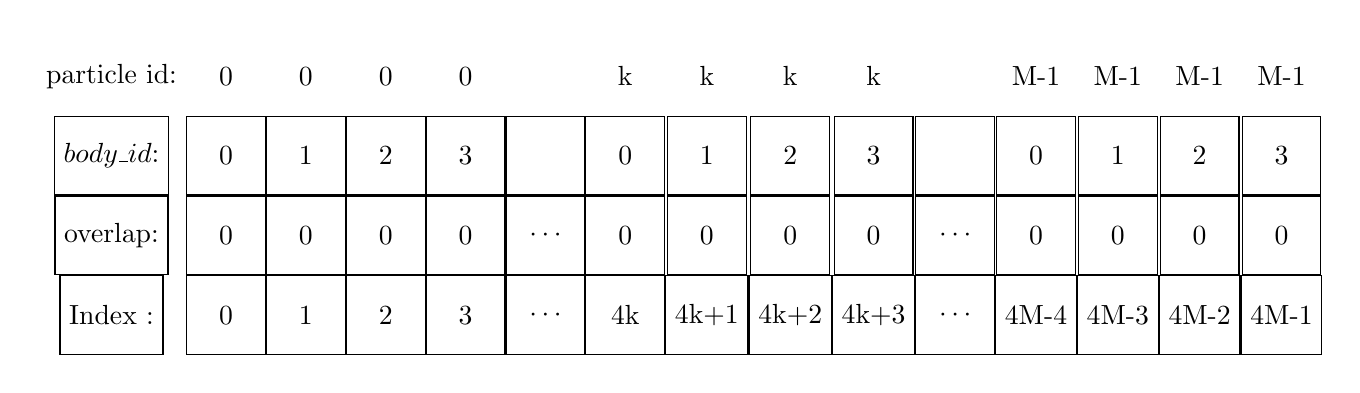
\begin{tikzpicture}
    \matrix (m) [matrix of nodes,
    nodes={draw, minimum size=10mm,anchor=center},
    nodes in empty cells, minimum height = 1cm,
    row 1/.style={nodes={draw=none}},]
    {
      particle id: & 0 & 0 & 0 & 0 &          & k  & k    & k    & k    &          & M-1  & M-1  & M-1  & M-1 \\
      $body\_id$:  & 0 & 1 & 2 & 3 &          & 0  & 1    & 2    & 3    &          & 0    & 1    & 2    & 3 \\
      overlap:     & 0 & 0 & 0 & 0 & $\cdots$ & 0  & 0    & 0    & 0    & $\cdots$ & 0    & 0    & 0    & 0\\
      Index  :     & 0 & 1 & 2 & 3 & $\cdots$ & 4k & 4k+1 & 4k+2 & 4k+3 & $\cdots$ & 4M-4 & 4M-3 & 4M-2 & 4M-1\\
    };
  \end{tikzpicture}
  \caption{An array to track the pairwise quantities. A stride of length $4$ is
    assigned to each particle to track the pairwise quantity.}
\label{fig:stride_index_trace}
\end{figure}

At an intermediate time $t_1$, let us assume particle with an index $k$ of body
$1$ is in contact with body $2$ and $l$ with body $3$. This can be seen in
\cref{fig:id:four_bodies_contact}. The updated overlap amount of particles $k$
and $l$ is given in \cref{fig:id:k_f_overlap_t_1},
\begin{figure}[!htpb]
  \centering
  \footnotesize
  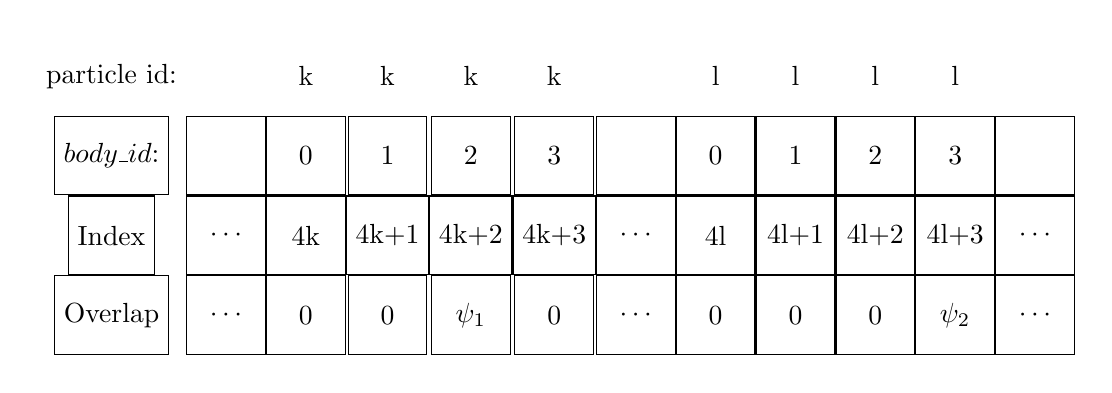
\begin{tikzpicture}
    \matrix (m) [matrix of nodes,
    nodes={draw, minimum size=10mm,anchor=center},
    nodes in empty cells, minimum height = 1cm,
    row 1/.style={nodes={draw=none}},]
    {
      particle id: & & k & k & k & k & & l & l & l & l &  \\
      $body\_id$:  & & 0 & 1 & 2 & 3 & & 0 & 1 & 2 & 3 &  \\
      Index & $\cdots$ & 4k & 4k+1 & 4k+2 & 4k+3 & $\cdots$ & 4l & 4l+1 & 4l+2 & 4l+3 & $\cdots$ \\
      Overlap & $\cdots$ & 0 & 0 & $\psi_1$ & 0 & $\cdots$ & 0 & 0 & 0 & $\psi_2$ & $\cdots$ \\
    };
  \end{tikzpicture}
  \caption{Updated overlap amount of particles $k$ and $l$.}
\label{fig:id:k_f_overlap_t_1}
\end{figure}
where $\psi$ in the figure is a real number. Since particle $k$ is in contact
with body id $2$, we can see from \cref{fig:id:k_f_overlap_t_1} that the overlap
amount of particle $k$ with body id $2$ is saved as $\psi_1$. This overlap
amount is saved at its fixed array index of $4k+2$. Since particle $l$ is in
contact with body id $3$, we save the overlap with body $3$ at $4k+3$ index.
Similarly, let us assume a particle with an index $q$ is in contact with the
body $2$ and $3$. The pairwise array belonging to the particle $q$ is shown in
\cref{fig:id:overlap_of_q_at_t_1}. From \cref{fig:id:overlap_of_q_at_t_1}, we
can see that the pairwise overlap quantity of particle $q$ with bodies $2$ and
$3$ are saved at the indices of $4q+2$ and $4q+3$, respectively.
\begin{figure}[!htpb]
  \centering
  \footnotesize
  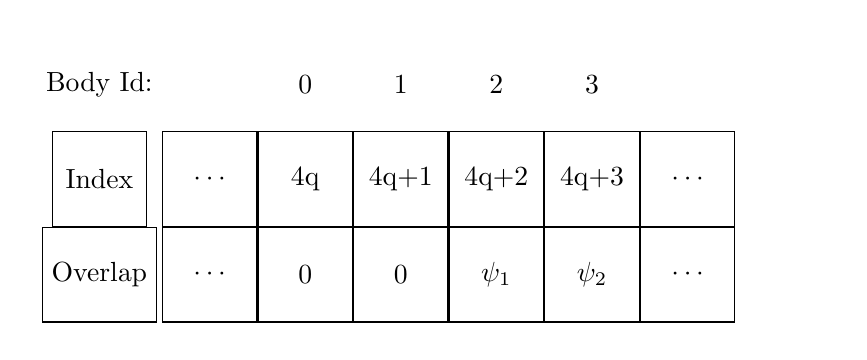
\begin{tikzpicture}
    \matrix (m) [matrix of nodes,
    nodes={draw, minimum size=12mm,anchor=center},
    nodes in empty cells, minimum height = 1cm,
    row 1/.style={nodes={draw=none}},]
    {
      Body Id: & & 0 & 1 & 2 & 3 & & \\
      Index & $\cdots$ & 4q & 4q+1 & 4q+2 & 4q+3 & $\cdots$ \\
      Overlap & $\cdots$ & 0 & 0 & $\psi_1$ & $\psi_2$ & $\cdots$ \\
    };
  \end{tikzpicture}
  \caption{Overlap amount of particle $q$ when in contact with bodies $2$ and $3$.}
  \label{fig:id:overlap_of_q_at_t_1}
\end{figure}

At the time ($t_3$), let the particle $l$ lose its collision with body $3$,
while particle $k$ is still in contact with body $2$. The updated overlap array
for this configuration is shown in \cref{fig:id:overlap_of_k_f_at_t_2}. From
\cref{fig:id:overlap_of_k_f_at_t_2}, we can see that we have updated the
pairwise tracking quantity, overlap, we make the overlap array value at index
$4l+3$ zero, as the particle $l$ lost contact with body $3$. However, we keep
the overlap value of particle $k$ with body $2$ since it didn't lose contact
with it.

\begin{figure}[!htpb]
  \centering
  \footnotesize
  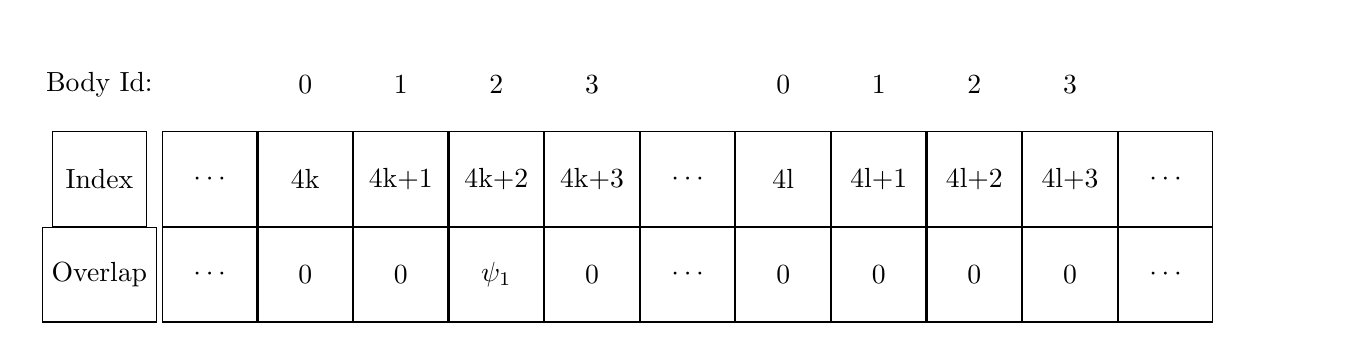
\begin{tikzpicture}
    \matrix (m) [matrix of nodes,
    nodes={draw, minimum size=12mm,anchor=center},
    nodes in empty cells, minimum height = 1cm,
    row 1/.style={nodes={draw=none}},]
    {
      Body Id: & & 0 & 1 & 2 & 3 & &  0 & 1 & 2 & 3 & & \\
      Index & $\cdots$ & 4k & 4k+1 & 4k+2 & 4k+3 & $\cdots$ & 4l & 4l+1 & 4l+2 & 4l+3 & $\cdots$ \\
      Overlap & $\cdots$ & 0 & 0 & $\psi_1$ & 0 & $\cdots$ & 0 & 0 & 0 & 0 & $\cdots$ \\
    };
  \end{tikzpicture}
  \caption{Overlap array of body $1$, showing the specific indices of
    particles $k$ and $l$ at time $t_2$.}
\label{fig:id:overlap_of_k_f_at_t_2}
\end{figure}
While letting particle $q$ lose its contact with bodies $2$ and $3$ and come
into contact with body $0$. In this case, the updated overlap array for the
indices belonging to the particle $q$ is given in
\cref{fig:id:overlap_of_q_at_t_2}. Similar to particle $k$ and $l$, we update
the pairwise tracking quantity, however, we save the overlap amount of particle
$q$ with body $0$ and make overlap amounts to zero for the indices of $4q+2$ and
$4q+3$.
\begin{figure}[!htpb]
  \centering
  \footnotesize
  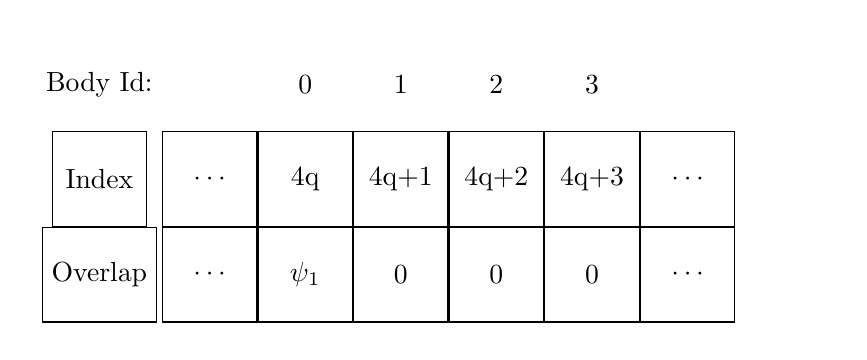
\begin{tikzpicture}
    \matrix (m) [matrix of nodes,
    nodes={draw, minimum size=12mm,anchor=center},
    nodes in empty cells, minimum height = 1cm,
    row 1/.style={nodes={draw=none}},]
    {
      Body Id: & & 0 & 1 & 2 & 3 & & \\
      Index & $\cdots$ & 4q & 4q+1 & 4q+2 & 4q+3 & $\cdots$ \\
      Overlap & $\cdots$ & $\psi_1$ & 0 & 0 & 0 & $\cdots$ \\
    };
  \end{tikzpicture}
  \caption{Overlap array of body $1$, showing the index of
    particle $q$ at time $t_2$.}
\label{fig:id:overlap_of_q_at_t_2}
\end{figure}
In the next section we look at the code to implement this algorithm in
PySPH.

\FloatBarrier%
\subsection{Implementation in PySPH}
We implement the above algorithm in PySPH using the following code. We first
create a particle array with the required properties. A sample code segment
describing the creation of a particle array is given as
\lstset{caption={Code segment for the creation of a particle array.}} \lstset{basicstyle=\footnotesize\ttfamily}
\begin{lstlisting}[label={contact:equations},frame=lines,language=Python,upquote=True]
body_2 = get_particle_array(x=[0., 1., 2., 3.],
                            y=[0., 0., 0., 0.],
                            m=m,
                            rho=rho,
                            ...=...
                            name="body")
\end{lstlisting}

To implement the pairwise tracking algorithm, we add an additional property with
a stride. In our case, a particle can contact four bodies at a given time. A
property of stride length $4$ is added to the particle array as
\lstset{caption={Code segment to add a stride property to an existing particle
    array.}} \lstset{basicstyle=\footnotesize\ttfamily}
\begin{lstlisting}[label={contact:equations},frame=lines,language=Python,upquote=True]
body_2.add_property(name='overlap', stride=4)
\end{lstlisting}
The pairwise interactions are computed with the following code
\lstset{caption={Code snippet to handle tracking of pairwise interactions with a few number of bodies.}} \lstset{basicstyle=\footnotesize\ttfamily}
\begin{lstlisting}[label={contact:equations},frame=lines,language=Python,upquote=True]
class ComputeContactForce(Equation):
    def initialize(self, d_idx, d_overlap, d_total_no_bodies, dt, t):
        i, t1, t2 = declare('int', 3)

        t1 = d_total_no_bodies[0] * d_idx

        for i in range(d_total_no_bodies[0]):
            t2 = t1 + i
            d_overlap[t2] = 0.

    def loop(self, d_idx, d_total_no_bodies, s_idx,
            s_body_id, dt, RIJ):
        t1, t2 = declare('int', 2)

        t1 = d_total_no_bodies[0] * d_idx
        t2 = t1 + s_body_id[s_idx]

        d_overlap[t2] += RIJ
        # ... Code redacted ...
\end{lstlisting}
Here, \textit{d\_total\_no\_bodies} is the total number of bodies that consist
in a given case. In the above code listing, in order to compute the overlap of
the particles on a given body with the other bodies, we first initialize the
pairwise quantity, overlap, to zero. $initialize$ method depicts the
initialization of overlap to zero. In $loop$ method, we compute the pairwise
overlap of the particle when colliding with the bodies. We compute the forces on
the bodies using the above equation using the $Group$ function in PySPH
$Application$ class routine as,
\lstset{caption={Code segment to compute the forces on the bodies.}} \lstset{basicstyle=\footnotesize\ttfamily}
\begin{lstlisting}[label={contact:equations},frame=lines,language=Python,upquote=True]
  Group(equations=[
      ComputeContactForce(dest='body_0', sources=[
          'body_1', 'body_2', 'body_3']),
      ComputeContactForce(dest='body_1', sources=[
          'body_1', 'body_2', 'body_3']),
      ComputeContactForce(dest='body_2', sources=[
          'body_1', 'body_2', 'body_3']),
      ComputeContactForce(dest='body_3', sources=[
          'body_0', 'body_1', 'body_2'])
    ])
\end{lstlisting}
We execute the equation of computation of the contact force of each body due to the
$sources$. Four equations are used to compute the forces on four bodies due to
the interaction with the other three bodies.


\FloatBarrier%
\section{Contact force modeling with a large number of particles}
\label{sec:tracking-many-bodies}
In the previous section, we used a strided array with a fixed index per
interaction to handle the tracking of pairwise interactions while computing the
contact force on a particle due to the interaction with other bodies. However, a
fixed index per interaction is not favorable when dealing with simulations
involving a large number of bodies or particles. This is because, a very large
stride is wasteful in terms of memory. For cases with a large number of bodies,
we propose an algorithm where dynamic addition and removal of contacts are
involved. Further, this algorithm is feasible in cases when the particle at a
given time will not have more than a fixed number of contacts to track. In the
current section, we demonstrate the dynamic contact handling algorithm. We
consider two cases, one where all the particles belong to the same particle
array and another case where particles belonging to two different particle
arrays interact with each other and among themselves.

\subsection{Single particle array}
\begin{figure}[!htpb]
  \centering
  \includegraphics[width=0.3\textwidth]{images/implementation_detail/images/many_bodies/many_bodies_t_0}
  \caption{Particles with finite radius at time $t=0$.}
\label{fig:id:15_particle_t_0}
\end{figure}

To demonstrate the dynamic tracking algorithm, we consider the interaction of
$15$ particles as shown in \cref{fig:id:15_particle_t_0}. We assume, at a given
time, no particle can have more than $3$ contacts. We demonstrate the algorithm
when the particles are initiated in a single particle array, such that no two
particles have the same index. Since, with a large number of bodies involved, we
do not have a prefixed index for the pairwise interaction, we additionally need
to save the index of the contacting particle in addition to the pairwise contact
properties. \Cref{fig:many_bodies_initialize_overlap_t_0}, shows the additional
property, $contact id$, added to the particle array to track the indices which a
given particle of index $k$ is in contact with. The contact indices are
initialized to $-1$ and other pairwise interaction properties are initialized to
$0$ similar to the previous algorithm.
\begin{figure}[!htpb]
  \centering
  \footnotesize
  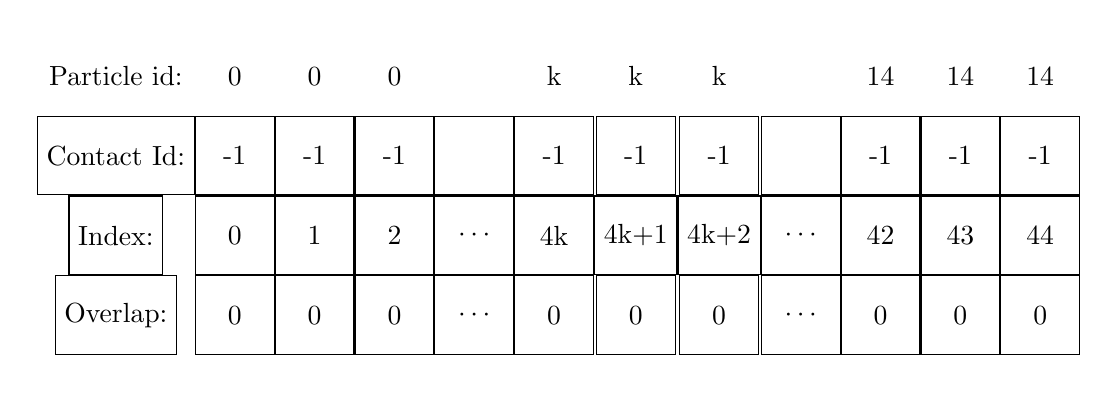
\begin{tikzpicture}
    \matrix (m) [matrix of nodes,
    nodes={draw, minimum size=10mm,anchor=center},
    nodes in empty cells, minimum height = 1cm,
    row 1/.style={nodes={draw=none}},]
    {
      Particle id: & 0 & 0 & 0 & & k & k & k & & 14 & 14  & 14 \\
      Contact Id: & -1 & -1 & -1 &  & -1 & -1 & -1 & & -1 & -1 & -1  \\
      Index: & 0 & 1 & 2 & $\cdots$ & 4k & 4k+1 & 4k+2 & $\cdots$ & 42 & 43 & 44 \\
      Overlap: & 0 & 0 & 0 & $\cdots$ & 0 & 0 & 0 & $\cdots$ & 0 & 0 & 0 \\
    };
  \end{tikzpicture}
  \caption{Values of strided array properties to handle the tracking of many bodies at time $t=0$.}
\label{fig:many_bodies_initialize_overlap_t_0}
\end{figure}

Code fragment of adding the new stride properties is given as
\lstset{caption={Code fragment to add the property required to track dynamics contacts.}} \lstset{basicstyle=\footnotesize\ttfamily}
\begin{lstlisting}[label={contact:equations},frame=lines,language=Python,upquote=True]
  pa.add_property('contact_id', stride=3, type="int")
  pa.contact_id[:] = -1
  pa.add_property(name='overlap', stride=3)
\end{lstlisting}

\begin{figure}[!htpb]
  \centering
  \includegraphics[width=0.3\textwidth]{images/implementation_detail/images/many_bodies/many_bodies_t_1}
  \caption{Configuration of particles at an intermediate time $t_1$.}
\label{fig:id:15_particle_t_1}
\end{figure}
%
The configuration of particles at an intermediate time $t_1$ are shown in
\cref{fig:id:15_particle_t_1}. Particles marked in red are contacts of $1$, $8$,
and $11$ indices. From \cref{fig:id:15_particle_t_1}, we can see that
particle with index $1$ is in contact with $0, 6, 7$ particles and a particle
with index $8$ with $5$ and $9$. Let us assume the contacts are formed for the
first time. \Cref{fig:many_bodies_initialize_overlap_1_8_11_t_1} shows the
updated overlap array of the contact indices, including the overlap for the
particles with index $1, 8$, and $11$.
\begin{figure}[!htpb]
  \centering
  \footnotesize
  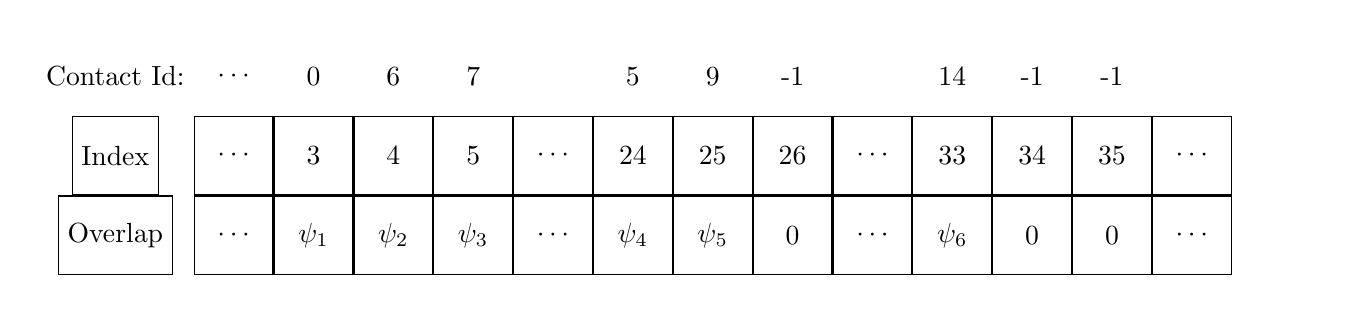
\begin{tikzpicture}
    \matrix (m) [matrix of nodes,
    nodes={draw, minimum size=10mm,anchor=center},
    nodes in empty cells, minimum height = 1cm,
    row 1/.style={nodes={draw=none}},]
    {
      Contact Id: & $\cdots$ & 0 & 6 & 7 &  & 5 & 9 & -1 & & 14 & -1 & -1 & & \\
      Index & $\cdots$ & 3 & 4 & 5 & $\cdots$ & 24 & 25 & 26 & $\cdots$ & 33 & 34 & 35 & $\cdots$\\
      Overlap  &$\cdots$ & $\psi_1$ & $\psi_2$ & $\psi_3$ & $\cdots$ & $\psi_4$ & $\psi_5$ & 0 & $\cdots$ & $\psi_6$ & 0 & 0 & $\cdots$ \\
    };
  \end{tikzpicture}
  \caption{Updated Contact Id and Overlap array at an intermediate time $t_1$.}
\label{fig:many_bodies_initialize_overlap_1_8_11_t_1}
\end{figure}

Dynamic pairwise contact tracking is handled in two parts. The first part is to
remove any contact particle that is previously in contact with and is no more in
contact. As a second step, we add new contacts. To implement this in PySPH, we
use two equations. One is to add new contacts and update the value of the
existing contacts, while the second one is to remove particle indices that are
no more in contact. We outline the code to add new contacts and update the
existing ones in the following code snippet.
\lstset{caption={Code snippet to add new contact and update existing contact properties in dynamic pairwise tracking algorithm.}} \lstset{basicstyle=\footnotesize\ttfamily}
\begin{lstlisting}[label={code:add_contacts_many},frame=lines,language=Python,upquote=True]
class AddParticlesInContact(Equation):
    def loop(self, d_idx, d_m, d_contact_id, d_overlap, d_total_contacts,
             d_max_contacts_limit, RIJ, d_rad, s_idx, s_rad):
        p, q1, tot_ctcs, j, found_at, found = declare('int', 6)
        overlap = -1.

        # check the particles are not on top of each other.
        if RIJ > 1e-12:
            overlap = d_rad[d_idx] + s_rad[s_idx] - RIJ

        # ---------- force computation starts ------------
        # if particles are overlapping
        if overlap > 0:
            # total number of contacts of particle i in destination
            tot_ctcs = d_total_contacts[d_idx]

            # d_idx has a range of tracking indices with sources
            # starting index is p
            p = d_idx * d_max_contacts_limit[0]
            # ending index is q -1
            q1 = p + tot_ctcs

            # check if the particle is in the tracking list
            # if so, then save the location at found_at
            found = 0
            for j in range(p, q1):
                if s_idx == d_contact_id[j]:
                    found_at = j
                    found = 1
                    break
            # if the particle is not been tracked then assign an
            # index in tracking history.
            if found == 0:
                found_at = q1
                d_contact_id[found_at] = s_idx
                d_total_contacts[d_idx] += 1

            # implies we are tracking the particle
            else:
                # Save the pair wise quantity at found_at
                d_overlap[found_at] = overlap
\end{lstlisting}


\begin{figure}[!htpb]
  \centering
  \includegraphics[width=0.3\textwidth]{images/implementation_detail/images/many_bodies/many_bodies_t_2}
  \caption{configuration of particles at time $t_2$.}
\label{fig:id:15_particle_t_2}
\end{figure}

\Cref{fig:id:15_particle_t_2} shows the particles positions at time $t_2$. From
\cref{fig:id:15_particle_t_2}, we can see that a few particles lose contacts, and
a few gain new contacts. We will add the new particles to the tracking array
using the above code. However, after every time step, we need to update the
tracking array by removing particle indices that are no more in contact before
adding new contacts. \Cref{fig:many_bodies_initialize_overlap_1_8_11_t_2} shows
the updated contact indices array and the overlapping array at time $t_2$.
\begin{figure}[!htpb]
  \centering
  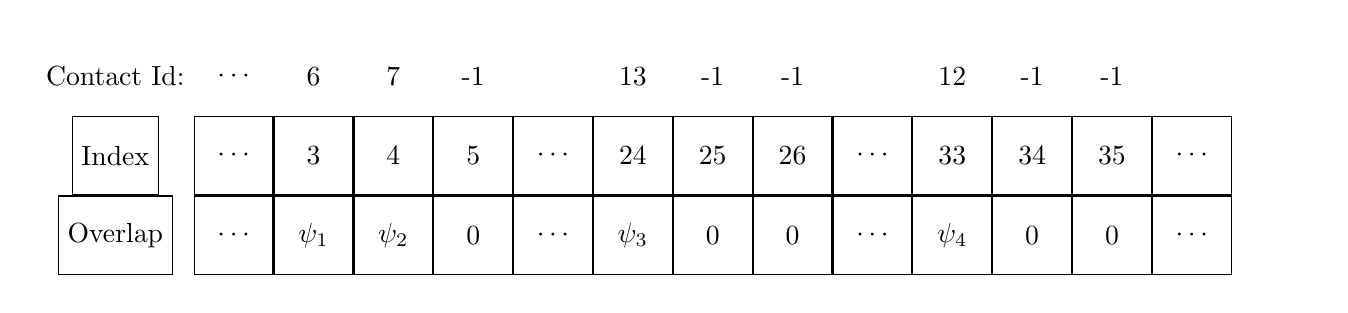
\begin{tikzpicture}
    \matrix (m) [matrix of nodes,
    nodes={draw, minimum size=10mm,anchor=center},
    nodes in empty cells, minimum height = 1cm,
    row 1/.style={nodes={draw=none}},]
    {
      Contact Id: & $\cdots$ & 6 & 7 & -1 &  & 13 & -1 & -1 & & 12 & -1 & -1 & & \\
      Index & $\cdots$ & 3 & 4 & 5 & $\cdots$ & 24 & 25 & 26 & $\cdots$ & 33 & 34 & 35 & $\cdots$\\
      Overlap  &$\cdots$ & $\psi_1$ & $\psi_2$ & 0 & $\cdots$ & $\psi_3$ & 0 & 0 & $\cdots$ & $\psi_4$ & 0 & 0 & $\cdots$ \\
    };
  \end{tikzpicture}
  \caption{Updated Contact Id and Overlap array at an intermediate time $t_2$}
\label{fig:many_bodies_initialize_overlap_1_8_11_t_2}
\end{figure}

The following code snippet is used to remove the contacts that are no more in
contact with the particle.
\lstset{caption={Code snippet to remove lost contacts in
dynamic pairwise tracking algorithm.}} \lstset{basicstyle=\footnotesize\ttfamily}
\begin{lstlisting}[label={contact:equations},frame=lines,language=Python,upquote=True]
class RemoveParticlesNotInContact(Equation):
    def initialize_pair(self, d_idx, d_x, d_y, d_z, d_rad,
                        d_total_contacts, d_contact_id,
                        d_max_contacts_limit, d_overlap,
                        s_rad):
        # Declare variable: Code redacted

        idx_total_ctcs = d_total_contacts[d_idx]
        # particle idx contacts has range of indices
        # and the first index would be
        p = d_idx * d_max_contacts_limit[0]
        last_idx_tmp = p + idx_total_ctcs - 1
        k = p
        count = 0

        # loop over all the contacts of particle d_idx
        while count < idx_total_ctcs:
            # The index of the particle with which
            # d_idx in contact is
            sidx = d_contact_id[k]

            if sidx == -1:
                break
            else:
                xij[0] = d_x[d_idx] - s_x[sidx]
                xij[1] = d_y[d_idx] - s_y[sidx]
                xij[2] = d_z[d_idx] - s_z[sidx]
                rij = sqrt(xij[0] * xij[0] + xij[1] * xij[1] +
                           xij[2] * xij[2])

                overlap = d_rad_s[d_idx] + s_rad_s[sidx] - rij

                if overlap <= 0.:
                    # if the swap index is the current index then
                    # simply make it to null contact.
                    if k == last_idx_tmp:
                        d_contact_id[k] = -1
                        d_overlap[k] = 0.
                    else:
                        # swap the current tracking index with the final
                        # contact index
                        d_contact_id[k] = d_contact_id[last_idx_tmp]
                        d_contact_id[last_idx_tmp] = -1

                        # swap tangential x displacement
                        d_overlap[k] = d_overlap[last_idx_tmp]
                        d_overlap[last_idx_tmp] = 0.

                        # decrease the last_idx_tmp, since we swapped it to
                        # -1
                        last_idx_tmp -= 1

                    # decrement the total contacts of the particle
                    d_total_contacts[d_idx] -= 1
                else:
                    k = k + 1
                count += 1
\end{lstlisting}
The above equations are used in the $create\_equations$ method of $Application$
class of PySPH to execute in execution loop using the following code.
\lstset{caption={An equation execution order to handle the pairwise tracking algorithm in PySPH.}} \lstset{basicstyle=\footnotesize\ttfamily}
\begin{lstlisting}[label={contact:equations},frame=lines,language=Python,upquote=True]
  Group(equations=[
      RemoveParticlesNotInContact(dest='grains',
      sources=['grains'])
    ]),
  Group(equations=[
      AddParticlesInContact(dest='grains', sources=['grains'])
    ]),
\end{lstlisting}


\FloatBarrier%
\subsection{Dealing with multiple particle arrays}
Let us consider a case where particles of two different particle arrays
interact with each other. A schematic is shown in \cref{fig:mb:2_pa}. Here,
we consider each particle array to have $15$ particles, as shown in
\cref{fig:mb:2_pa}.
\begin{figure}[!htpb]
  \centering
  \includegraphics[width=0.7\textwidth]{images/implementation_detail/images/many_bodies/many_bodies_two_pa_t_0}
  \caption{}
\label{fig:mb:2_pa}
\end{figure}
Let's name particle array $1$ as $grains_1$ and particle array $2$ as $grains_2$.
As described in the previous section, in PySPH, to compute the interaction, we
use the following code snippet.
\lstset{caption={Code snipped to compute contact force on particle arrays.}} \lstset{basicstyle=\footnotesize\ttfamily}
\begin{lstlisting}[label={contact:equations},frame=lines,language=Python,upquote=True]
  Group(equations=[
      RemoveParticlesNotInContact(dest='grains_1',
          sources=['grains_1', 'grains_2'])
      RemoveParticlesNotInContact(dest='grains_2',
          sources=['grains_1', 'grains_2'])
    ]),
  Group(equations=[
      AddParticlesInContact(dest='grains_1',
          sources=['grains_1', 'grains_2'])
      AddParticlesInContact(dest='grains_2',
          sources=['grains_1', 'grains_2'])
    ]),
\end{lstlisting}


Let us consider the computation of contact force on particles belonging to
particle array 1. From the previous algorithm, we initialize the $contact\_id$
and $overlap$ arrays to particle array $1$ as shown in \cref{fig:mb-2-pa-prev-algo}.
\begin{figure}[!htpb]
  \centering
  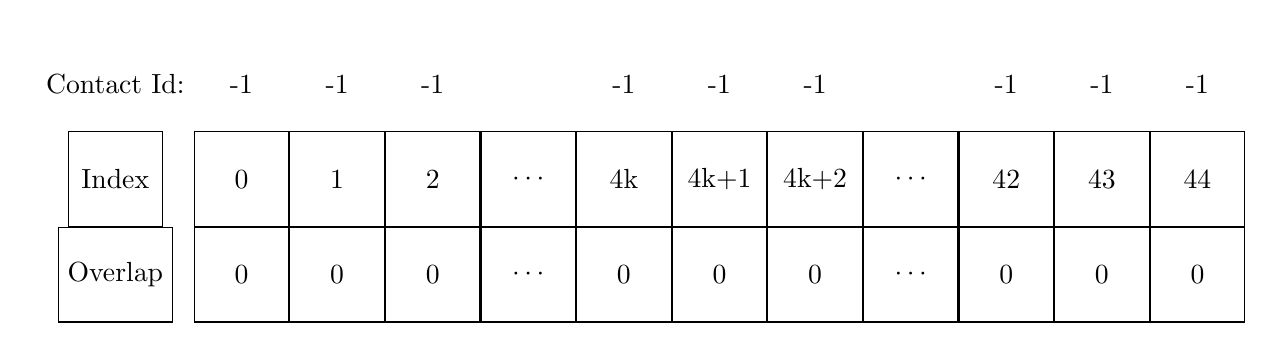
\begin{tikzpicture}
    \matrix (m) [matrix of nodes,
    nodes={draw, minimum size=12mm,anchor=center},
    nodes in empty cells, minimum height = 1cm,
    row 1/.style={nodes={draw=none}},]
    {
      Contact Id: & -1 & -1 & -1 &  & -1 & -1 & -1 & & -1 & -1 & -1  \\
      Index & 0 & 1 & 2 & $\cdots$ & 4k & 4k+1 & 4k+2 & $\cdots$ & 42 & 43 & 44 \\
      Overlap & 0 & 0 & 0 & $\cdots$ & 0 & 0 & 0 & $\cdots$ & 0 & 0 & 0 \\
    };
  \end{tikzpicture}
  \caption{Contact Id and Overlap array for particle array 1.}
\label{fig:mb-2-pa-prev-algo}
\end{figure}

\Cref{fig:mb-2-pa-t-2} shows the particle arrays' particles
interacting with each other. From \cref{fig:mb-2-pa-t-2}, we can see particles
of both arrays interact with each other. \cref{fig:zoomed-8-id} depicts
contacts of particle with index $8$. The contact array and the pairwise overlap
of a particle with index $8$ are shown in \cref{fig:id-8-mb-array}. From
\cref{fig:id-8-mb-array,fig:zoomed-8-id}, we can see that the particle with
index $8$ is in contact with a particle of index $5$ of both the particle arrays
and with $1$ of particle array 2. The algorithm developed for a single particle
array fails to identify the contact properly, as there is no way to
differentiate between which particle array the given contacting particle belongs.
\begin{figure}[!htpb]
  \centering
  \includegraphics[width=0.5\textwidth]{images/implementation_detail/images/many_bodies/many_bodies_two_pa_t_1}
  \caption{Configuration of the particles at an intermediate time $t_1$.}
\label{fig:mb-2-pa-t-2}
\end{figure}
\begin{figure}[!htpb]
  \centering
  \includegraphics[width=0.2\textwidth]{images/implementation_detail/images/many_bodies/many_bodies_two_pa_t_1_zoomed}
  \caption{Contacts of particle with index $8$ with particles with index $5$
    both the particle arrays and index $1$.}
\label{fig:zoomed-8-id}
\end{figure}
\begin{figure}[!htpb]
  \centering
  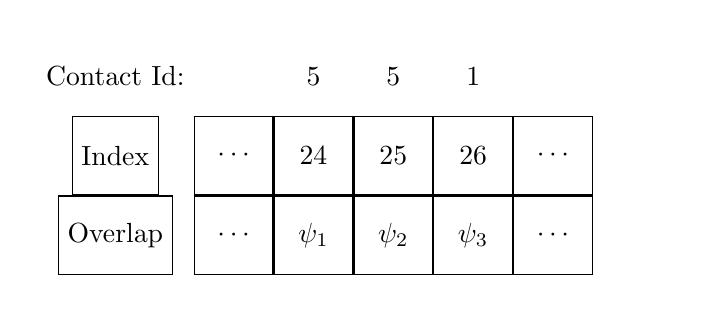
\begin{tikzpicture}
    \matrix (m) [matrix of nodes,
    nodes={draw, minimum size=10mm,anchor=center},
    nodes in empty cells, minimum height = 1cm,
    row 1/.style={nodes={draw=none}},]
    {
      Contact Id: & & 5 & 5 & 1 & & \\
      Index & $\cdots$ & 24 & 25 & 26 & $\cdots$\\
      Overlap  &$\cdots$ & $\psi_1$ & $\psi_2$ & $\psi_3$ & $\cdots$\\
    };
  \end{tikzpicture}
  \caption{Updated Contact Id and Overlap array at an intermediate time $t_1$,
    showing indices for particle $8$.}
\label{fig:id-8-mb-array}
\end{figure}

To solve this issue, we assign an additional property to the particles, a unique
id, to each different particle array. Such as, here, we would add a property
named $unique\_id$, where for each particle array, we would assign a unique id.
The updated tracking properties with the $unique\_id$ included is shown in
\cref{fig:mb-ui-included}.
\begin{figure}[!htpb]
  \centering
  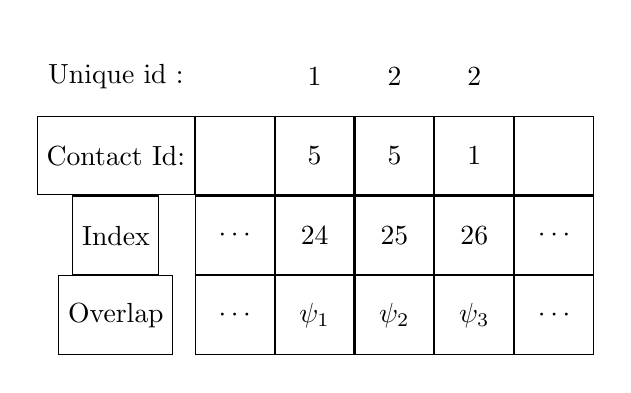
\begin{tikzpicture}
    \matrix (m) [matrix of nodes,
    nodes={draw, minimum size=10mm,anchor=center},
    nodes in empty cells, minimum height = 1cm,
    row 1/.style={nodes={draw=none}},]
    {
      Unique id : & & 1 & 2 & 2 & \\
      Contact Id: & & 5 & 5 & 1 & \\
      Index & $\cdots$ & 24 & 25 & 26 & $\cdots$\\
      Overlap  &$\cdots$ & $\psi_1$ & $\psi_2$ & $\psi_3$ & $\cdots$\\
    };
  \end{tikzpicture}
  \caption{Updated tracking properties of particle $8$ with unique id included.}
\label{fig:mb-ui-included}
\end{figure}
The updated code, with multiple particle arrays reads,
\lstset{caption={Code snippet to add new contact and update existing contact properties in
dynamic pairwise tracking algorithm with multiple particle arrays.}} \lstset{basicstyle=\footnotesize\ttfamily}
\begin{lstlisting}[label={contact:equations},frame=lines,language=Python,upquote=True]
class TrackTheOverlap(Equation):
    def loop(self, d_idx, d_m, d_contact_id, d_overlap, d_total_contacts,
            d_max_contacts_limit, RIJ, d_rad, s_idx, s_rad
            s_unique_id, d_contact_unique_idx):
        p, q1, tot_ctcs, j, found_at, found = declare('int', 6)
        overlap = -1.

        # check the particles are not on top of each other.
        if RIJ > 1e-12:
            overlap = d_rad[d_idx] + s_rad[s_idx] - RIJ

        # ---------- force computation starts ------------
        # if particles are overlapping
        if overlap > 0:
            # total number of contacts of particle i in destination
            tot_ctcs = d_total_contacts[d_idx]

            # d_idx has a range of tracking indices with sources
            # starting index is p
            p = d_idx * d_max_contacts_limit[0]
            # ending index is q -1
            q1 = p + tot_ctcs

            # check if the particle is in the tracking list
            # if so, then save the location at found_at
            found = 0
            for j in range(p, q1):
                if s_idx == d_contact_id[j] and \
                   s_unique_id[s_idx] == d_contact_unique_idx[j]:
                    found_at = j
                    found = 1
                    break
            # if the particle is not been tracked then assign
            # an index in tracking history.
            if found == 0:
                found_at = q1
                d_contact_id[found_at] = s_idx
                d_contact_unique_idx[found_at] = s_unique_id[s_idx]
                d_total_contacts[d_idx] += 1

            # implies we are tracking the particle
            else:
                # Save the pair wise quantity at found_at
                d_overlap[found_at] = overlap
\end{lstlisting}
In the above code, we have additionally added a check to the existing single
particle array code. This check ensures that the indices we are tracking belong
to the correct particle array.


\FloatBarrier%
\subsection{Sand in a Rotating Drum}
\label{sec:dem-drum-case}
This example demonstrates the implementation in simulating motion of sand in a
rotating drum. The algorithms discussed in \cref{sec:tracking-many-bodies} are
used to handle the contact between the sand particles. The dynamics of the
particles follow the formulation by \cite{cundall_discrete_1979} and
\cite{luding_dem_2008}. The drum is initially static and starts rotating with an
angular velocity of 5 rad/s after the sand settles down. Figure 14 shows the
arrangement of the sand particles, the top row depicts the results when the drum
is not rotating, while the bottom row is when the drum is rotating. This shows
that PySPH provides the features required to implement a variety of different
meshless methods.
\begin{figure}
  \centering
  \includegraphics[width=0.6\textwidth]{images/implementation_detail/images/many_bodies/dem_rolling_drum_case}
  \caption{Positions of the sand in a drum, color indicates the velocity magnitude. The top row depicts the
results when the drum is not rotating, and the bottom row is when the drum is rotating.}
\label{fig:dem_drum}
\end{figure}


\FloatBarrier%
\section{Sub-stepping update algorithm}
\label{sec:substepping-algorithm}
Problems involving two different materials, such as fluid-structure interaction,
rigid-fluid coupling, etc., involve solving two different materials, such that
one material is stiffer than the other. Let us consider a problem that has both
fluid and solid. Assume timesteps of fluid and solid are related as follows,
\begin{equation}
\Delta t_f = K \Delta t_s,
\end{equation}
where $K$ is some integer. We use a sub-stepping integration scheme to update
the state of $fluid$ and $solid$ particles. Let us say $fluid$ has $10,000$
particles, and the solid has $1000$ particles, and let $K$ be $10$. Using a
sub-stepping scheme, instead of iterating $10,000$ particles $10$ times, we only
do it one time. We first move the higher timestep material to the next time
step, here fluid, then update the material with lower timestep in $K$ times,
such that the simulation is stable.
\begin{figure}[!htpb]
  \centering
  \includegraphics[width=1.0\textwidth]{images/implementation_detail/images/multiphase/time_stepping}
  \caption{Pictorial representation of the sub-stepping algorithm.}
\label{fig:id:multiphase}
\end{figure}
\Cref{fig:id:multiphase} depicts idea of sub-stepping algorithm. Here,
$\Delta t_{\text{factor}}$ is choosen as a timestep for $solid$ particles.
$\Delta t_{\text{factor}}$ is computed based on two factors. One is it is a
integer multiple of $\Delta t_{\text{material 1}}$
(\cref{eqn:id:dt_factor_chose}) and the second is it has to be less than or
equal to $\Delta t_{\text{material 2}}$, such that the simulation is stable.
\begin{equation}
\label{eqn:id:dt_factor_chose}
\Delta t_{\text{factor}} = \frac{\Delta t_{\text{material 1}}}{K}
\end{equation}


\FloatBarrier%
\subsection{Implementation in PySPH}
\label{sec:pysph-substepping-algorithm}
The following integrator routine is used for the sub-stepping algorithm
\lstset{caption={Code snippet for integrator used in substepping.}}
\lstset{basicstyle=\footnotesize\ttfamily}
\begin{lstlisting}[label={contact:equations},frame=lines,language=Python,upquote=True]
class SubSteppingIntegrator(Integrator):
    def one_timestep(self, t, dt):
        self.compute_accelerations()
\end{lstlisting}
We can see that only one method $self.compute\_accelerations()$ is
called at every timestep in a sub-stepping scheme. We use the PySPH feature of
being able to iterate a group of equations to implement this algorithm. We
iterate using the larger $\Delta t$ value, but inside that, we use an iterated
loop with the smaller timestep. The code listing of updating the particle
arrays with different timesteps is given as,
\lstset{caption={Code snippet for substepping algorithm in PySPH.}}
\lstset{basicstyle=\footnotesize\ttfamily}
\begin{lstlisting}[label={contact:equations},frame=lines,language=Python,upquote=True]
  Group(equations=[
      FluidEquations(dest='fluid', sources=['fluid', 'solid'],
                     dt=dt_1)
  ]),
  Group(equations=[
      Group(equations=[
          SolidEquations(dest='solid', sources=['fluid', 'solid'],
                         dt=dt_1/K)
      ])
  ]
  iterate=True, max_iterations=10, min_iterations=10)
\end{lstlisting}
Since here, $fluid$ has a higher timestep, we first update it to the next
timestep using $FluidEquations$ and the $solid$ state is updated to $t + \Delta t_1$
timestep using $10$ updates with a timestep of $\frac{\Delta t_1}{K}$. At each
iteration we advance the $solid$ particles by $\Delta t_1 / K$ time using
$SolidEquations$ equations.


\FloatBarrier%
\section{Summary}
\label{sec:id:summary}
In the current chapter, we demonstrated the implementation details of the
algorithms developed in \cref{chap:ctvf,chap:csph}. The PySPH documentation has
implementation details of several algorithms implemented in the above chapters.
We discussed algorithms corresponding to the contact force interaction and
simulation involving two different materials with different timestep values.

A strided array approach is used to track the pairwise contacts. A fixed index
is assigned to the particle for each pairwise interaction with a few bodies
handled. In cases with many bodies, a similar strided approach is used. However,
the contacts are updated dynamically as the particles make and leave contacts.
\Cref{sec:contact-algorithm} utilizes the algorithm of contact tracking for
fewer bodies, while \cref{sec:dem-drum-case} follows the contact tracking
algorithm for many bodies.

A sub-stepping algorithm is discussed in which the material with a higher
timestep is updated first, then the stiffer phase is updated with a lower time
step but in $K$ intervals. We discussed the tools provided by PySPH in order to
implement the sub-stepping algorithm.

In the next chapter, we model the interaction between the fluid and the elastic
structure, fluid-structure interaction. We propose an updated Lagrangian model
by coupling the solver developed in \cref{chap:ctvf} to handle the
fluid-structure interaction problems.

\chapter{Fluid structure interaction}\label{chap:fsi}
\section{Introduction}
Till now we have developed solvers to model the fluid and elastic dynamics. With
in the abrasive water jet machining, the interaction between the fluid and the
rigid or elastic part is remained. In the current chapter we utilize the CTVF
scheme developed in \cref{chap:ctvf} for fluid and elastic dynamics is coupled to
handle the fluid structure interaction in the current chapter. Problems with
free surface and analytical solution are used to validate.


Fluid-structure interaction (FSI) is a common engineering problem that is seen
in daily life. Some examples include the deformation of the wind turbine blade
due to the fluid flow, the flow traversal due to the deflected blade, blood flow
in heart value, coastal engineering, and vortex-induced vibration
\citep{williamson2004vortex,bearman2011circular}. An accurate study of FSI can
allow us to optimize the systems where FSI is dominant. However, studying the
FSI phenomena through experiments or analytical techniques is complex due to its
nonlinear behavior. % Therefore, a computational study is preferred which
% comprises of mesh-based and meshless methods.
% \todo{Re-write}



Handling FSI problems with the transport velocity formulation framework is
advantageous as it can solve the tensile instability issue in solid dynamics and
inhomogeneous particle distribution in fluids. In the current chapter, we handle
FSI problems by the CTVF method, where both fluids and solid phases are modeled
using CTVF alone. To validate the proposed method, we consider three numerical
test cases. A uniformly distributed load over a clamped beam (UDL) problem is
considered to validate the elastic dynamics of CTVF. An aluminum plate over a
hydrostatic tank for FSI validation is considered. Finally, it is applied to a
fluid flow hitting an elastic plate. Here, the deformation of the elastic plate
is compared against the experimental results. A convergence analysis is
undertaken for both UDL and elastic deformation under hydrodynamic load
problems. All the results are fully automated with the automan package
\citep{automan2018} and made hundred percent reproducible. The source code for
all the problems demonstrated in this manuscript is made available at
\url{https://github.com/dineshadepu/fsi_etvf}.

\section{Methodology}\label{sec2}

We follow CTVF formulation to model the fluid and solid phase. Following CTVF,
the particles are moved with a transport velocity rather than the momentum
velocity, with which we get a homogenized particle distribution as well as it
eliminates the tensile instability. In the next two sections we show the
discretized equations of both fluid and solid phase. Please see
\citep{adepu2021corrected} for more details.

\subsection{Discrete equations of the fluid medium}\label{subsec:discrete-fluid}

The governing equations of the fluid are conservation of mass and momentum.
Following the weakly compressible SPH scheme, we use an equation of state to
complete the system. The SPH discretization of the continuity
equation~\eqref{eq:sph-discretization-continuity} and the EDAC
based~\citepp{PRKP:edac-sph-iccm2015} pressure evolution
equation~\eqref{eq:sph-discretization-edac} respectively are,
\begin{equation}
  \label{eq:sph-discretization-continuity}
  \frac{\tilde{d}\rho_a}{dt} = \sum_{b} \; \frac{m_b}{\rho_{b}} \; (
  \rho_{a} \; \tilde{\ten{u}}_{ab} \; + \;
  (\rho \; (\tilde{\ten{u}} \; - \;
  \ten{u}))_{ab}) \; \cdot \nabla_{a} W_{ab},
\end{equation}
\begin{multline}
  \label{eq:sph-discretization-edac}
  \frac{\tilde{d}p_a}{dt} = \sum_{b} \; \frac{m_b}{\rho_{b}} \; \bigg(
  (p_{a} - \rho_{a} c_{s}^2) \; \ten{u}_{ab} \; + \;
  p_{a} \; \tilde{\ten{u}}_{ab} \; - \;
  (p \; (\tilde{\ten{u}} - \ten{u}))_{ab} \; + \; \\
  4 \; \nu_{edac}
  \frac{p_a - p_b}{(\rho_a + \rho_b) (r^2_{ab} + 0.01 h_{ab}^{2})} \ten{r}_{ab}
  \bigg) \; \cdot \nabla_{a} W_{ab}.
\end{multline}
%
Where $\frac{\tilde{d}}{dt}$ is the material derivative, with $\tilde{u}$ being
the transport velocity of the particles, $\ten{u}_{ab} = \ten{u}_a - \ten{u}_b$.
%
Similarly, the discretized momentum equation for fluids is written as,
\begin{multline}
  \label{eq:sph-momentum-fluid}
  \frac{\tilde{d}\ten{u}_{a}}{dt} = - \sum_{b} m_b \bigg[
  \bigg(\frac{p_a}{\rho_a^2} + \frac{p_b}{\rho_b^2}\bigg) \ten{I} -
  \bigg(\frac{\ten{A}_a}{\rho_a^2} + \frac{\ten{A}_b}{\rho_b^2} + \Pi_{ab}
  \ten{I} \bigg) \bigg]
  \cdot \nabla_{a} W_{ab} \\
  + \ten{u}_{a} \sum_{b} \frac{m_b}{\rho_{b}} \; \tilde{\ten{u}}_{ab} \cdot
  \nabla_{a} W_{ab} \\+ \sum_{b} m_b \frac{4 \eta \nabla W_{ab}\cdot
    \ten{r}_{ab}}{(\rho_a + \rho_b) (r_{ab}^2 + 0.01 h_{ab}^2)} \ten{u}_{ab} +
  \ten{g}_{a} + \frac{\ten{F}^a_{\text{FSI}}}{m_a}
\end{multline}
where $\ten{A}_a = \rho_a \ten{u}_a \otimes (\ten{\tilde{u}}_a - \ten{u}_a)$,
$\ten{I}$ is the identity matrix, $\eta$ is the kinematic viscosity of the
fluid and \citep{morris-lowRe-97} formulation is used to discretize the
viscosity term. $\Pi_{ab}$ is the artificial
viscosity~\citep{monaghan-review:2005} to maintain the stability of the
numerical scheme. It is given as,
\begin{align}
  \label{eq:mom-av}
  \Pi_{ab} =
  \begin{cases}
\frac{-\alpha h_{ab} \bar{c}_{ab} \phi_{ab}}{\bar{\rho}_{ab}}
  & \ten{u}_{ab}\cdot \ten{r}_{ab} < 0, \\
  0 & \ten{u}_{ab}\cdot \ten{r}_{ab} \ge 0,
\end{cases}
\end{align}
where,
%
\begin{equation}
  \label{eq:av-phiij}
  \phi_{ab} = \frac{\ten{u}_{ab} \cdot \ten{r}_{ab}}{r^2_{ab} + 0.01 h^2_{ab}},
\end{equation}
%
where, $\ten{r}_{ab} = \ten{r}_a - \ten{r}_b$, $h_{ab} = (h_a + h_b)/2$,
$\bar{\rho}_{ab} = (\rho_a + \rho_b)/2$, $\bar{c}_{ab} = (c_a + c_b) / 2$, and
$\alpha$ is the artificial viscosity parameter. $\ten{F}^a_{\text{FSI}}$ is the
force due to the interaction with elastic structure. This force modeling is
explained in \cref{subsec:fsi}. We utilize the ghost particle approach proposed
in \citep{Adami2012} to handle the boundaries.



\subsection{Solid phase modeling}\label{subsec:solid}
Similar to discretized fluid governing equation, the elastic structure equations are
\eqref{eq:sph-discretization-continuity}, and the momentum equation,
\begin{multline}
  \label{eq:sph-momentum-solid}
  \frac{\tilde{d}\ten{u}_{a}}{dt} = - \sum_{b} m_b \bigg[
  \bigg(\frac{p_a}{\rho_a^2} + \frac{p_b}{\rho_b^2}\bigg) \ten{I} -
  \bigg(\frac{\teng{\sigma}^{'}_{a}}{\rho_a^2} +
  \frac{\teng{\sigma}^{'}_{b}}{\rho_b^2} + \Pi_{ab} \ten{I} \bigg) \bigg]  \cdot \nabla_{a} W_{ab} \\
  + \ten{g}_{a} + \frac{\ten{F}^a_{\text{FSI}}}{m_a},
\end{multline}
while the additional stress terms, $\ten{A}$ in momentum equation of solid
mechanics are not considered as it has a negligible effect. An equation of state
is utilized to link the pressure with density following a weakly compressible
SPH scheme. Jaumann stress rate equation is solved to evolve the shear stress,
given as,
\begin{multline}
  \label{eq:sph-modified-jaumann-stress}
  \frac{\tilde{d}\teng{\sigma}^{'}_{a}}{dt} = 2G (\dot{\teng{\epsilon}}_{a} -
  \frac{1}{3} \dot{\teng{\epsilon}}_{a} \ten{I}) + \teng{\sigma}^{'}_{a}
  \teng{\Omega}_{a}^{T} +
  \teng{\Omega}_{a} \teng{\sigma}^{'}_{a}
\end{multline}
The SPH discretization of the
gradient of velocity is given as,
\begin{equation}
  \label{eq:sph-vel-grad}
  \nabla \ten{u}_a =
  - \sum_{b} \frac{m_b}{\rho_{b}} (\ten{u}_{a} - \ten{u}_{b}) \otimes (\nabla_{a} W_{ab}),
\end{equation}
where $\otimes$ is the outer product. With the strain and rotation tensors as,
\begin{equation}
  \label{eq:strain-tensor}
  \dot{\epsilon}_{ij} = \frac{1}{2} \bigg(\frac{\partial u_i}{\partial x_j} +
  \frac{\partial u_j}{\partial x_i} \bigg),
\end{equation}
and $\Omega_{ij}$ is the rotation tensor,
\begin{equation}
  \label{eq:rotational-tensor}
  \Omega_{ij} = \frac{1}{2} \bigg(\frac{\partial u_i}{\partial x_j} -
  \frac{\partial u_j}{\partial x_i} \bigg).
\end{equation}


\subsection{Transport velocity computation}\label{subsec:transport-velocity}
The particles in the current scheme are moved with the transport velocity,
\begin{equation}
  \label{eq:transport_velocity_position_derivative}
  \frac{d\ten{r}_a}{dt} = \ten{\tilde{u}}_a.
\end{equation}
%
The transport velocity is updated using,
\begin{equation}
  \label{eq:transport_velocity}
  \ten{\tilde{u}}_a(t + \Delta t) =\ten{u}_a(t) + \Delta t \; \frac{\tilde{d} \ten{u}_a}{dt} +
  \bigg(\frac{d \ten{u}_{a}}{dt}\bigg)_{\text{c}} \Delta t
\end{equation}

Where $\big(\frac{d \ten{u}_a}{dt}\big)_{\text{c}}$ is the homogenization
acceleration which ensures that the particle positions are homogeneous. In the
current work we have used Sun's \citep{sun_consistent_2019} PST to homogenization
the fluid medium while iterative PST (IPST)\citep{huang_kernel_2019} for the
solid phase. According to \citep{adepu2021corrected} the force formulation of
\citep{sun_consistent_2019} is,
\begin{equation}
  \label{eq:sun2019_pst}
  \bigg(\frac{d \ten{u}_a}{dt}\bigg)_{\text{c}} = - \frac{\text{M} \;
    (2h) c_0}{\Delta t} \sum_b \bigg[1 + R \bigg( \frac{W_{ab}}{W(\Delta x)} \bigg)^n
  \bigg] \nabla_a W_{ab} V_b,
\end{equation}
where $R$ is an adjustment factor to handle the tensile instability, and
$\text{M}$ is the mach number of the flow. $V_b$ is the volume of the
$b$\textsuperscript{th} particle, $c_0$ is the speed of sound. The acceleration is modified to account for
particles on the free surface. Here, $R = 0.2$ and $n = 4$ are used. Please see
\citep{adepu2021corrected} for detailed explanation of PST.

\subsection{Fluid-structure interaction}\label{subsec:fsi}
Coupling is handled in a straight forward way in SPH. While modelling the fluid
phase and treating the fluid-structure interactions, the structure particles are
assumed to be boundary particles. From the boundary handling given in Adami
\citep{Adami2012}, we compute the pressure of the boundary particles from
the extrapolated equation as,
\begin{equation}
  \label{eq:pressure-bc}
  p_s = \frac{\Sigma_f p_f W_{sf} + (\ten{g} - \ten{a}_{\ten{s}}) \cdot \Sigma_f
    \rho_f \ten{r}_{sf} W_{sf}}{\Sigma_f W_{sf}}.
\end{equation}
Here, $\ten{a}_s$ is the acceleration of the structure particles. The subscript
$f$ denotes the fluid particles and $s$ denotes the structure particles. By the
extrapolated pressure, hydrodynamic density of structure properties are
computed. Please note that the pressure we set here are only pertaining to the
FSI force and does not correspond to the real pressure or density of the
structure particles. By utilizing the previously set hydrodynamic properties on
the structure, the interaction force is computed using,
\begin{equation}
  \ten{F}_{\text{FSI}}^i = -m_i \sum_{a} m_a \bigg(\frac{p_i}{\rho_{i}^2} +
  \frac{p_a}{\rho_{a}^2} + \Pi_{ia} \bigg) \nabla_{i} W(x_{ia})
\end{equation}
where $i$ is fluid particle, $a$ is structure particle.


\section{Results And Discussion}\label{sec3}

% =========================================
% =========================================
% start
% =========================================
% =========================================
\subsection{Uniformly distributed loading (UDL) on a clamped beam}
\label{sec:udl}

In the first test case, we validate the structural part of the current solver.
We chose a homogeneous elastic plate clamped on both ends acted upon by a
uniformly distributed load ($q = 20$ Nm$\textsuperscript{-1}$) as shown in
\cref{fig:udl-schematic}. The beam's length (L) and height (H) is 0.2 m and
\begin{figure}
  \centering
  \includegraphics[scale=0.5]{images/fsi/images/khayyer_2021_udl/schematic}
  \caption{The schematic of a clamped elastic beam being acted upon by a
    uniformly distributed load.}
\label{fig:udl-schematic}
\end{figure}
$0.012$ m, respectively. The mechanical properties of the plate are set as
$E=10^7$ Pa in Young's modulus, $\nu=0$ in Poisson's ratio and $\rho=1000$
kgm$\textsuperscript{-3}$) in density. The numerical solution of the
y-displacement at the center of the beam is compared against the analytical
counterpart. The analytical solution for the deflection of a uniformly
distributed beam clamped at both ends is given by
\begin{equation}
  \label{eq:ce-tvf}
  \eta\left(\frac{L}{2}\right) = \frac{qL^4}{384 D},
\end{equation}
where, $D$ is defined as $\frac{E h^3}{12 (1 - (\nu)^2)}$. We consider three
particle resolutions such that, $10$, $15$, and $20$ particles along the beam's
width are used. We run for a total physical time of $2$ seconds.

\Cref{fig:udl-disp-plot} depicts the time history of y-displacement of the beam
center for different particle resolutions computed using the current solver
compared against the analytical solution. From \cref{fig:udl-disp-plot}, we can
see that the current solver can accurately predict the displacement of the
\begin{figure}
  \centering
  \includegraphics[scale=0.5]{figures/fsi/figures/khayyer_2021_udl/homogenous}
  \caption{Time variation of the y-displacement of the center of the beam for
    three different resolutions, compared against the analytical result.}
\label{fig:udl-disp-plot}
\end{figure}
clamped beam. Convergence of the current scheme is captured in
\cref{fig:udl-disp-plot}, and the computational results are within a reasonable
variation of the analytical solution with the variation of the particle spacing.


\subsection{Hydrostatic water column on an elastic plate}
\label{sec:hydrostatic-water-column-on-an-composite-elastic-plate}
In this example we study the deformation of an elastic plate due to the
hydrostatic water column. We utilise the current example to examine the accuracy
and convergence of the current solver. The schematic of fluid with the elastic
beam is shown in \cref{fig:hs-water-on-plate} along with the initial pressure
distribution in the fluid. The figure includes the dimensions as well. The
material properties of the beam are, a density of $2700$
kgm\textsuperscript{-3}, with an Young's modulus of $67.5$ GPa, and a Poisson
\begin{figure}
  \centering
  \includegraphics[scale=0.4]{images/fsi/images/ng_2020_hydrostatic_water_column_on_elastic_plate/schematic}
  \caption{Schematic of the hydrostatic water column on an elastic plate. Fluid
    particle color represents pressure.}
\label{fig:hs-water-on-plate}
\end{figure}
ratio of $0.34$. The material properties of the fluid are, a density of $1000$
kgm\textsuperscript{-3}, with a dynamic viscosity of $0$
kgm\textsuperscript{-1}s\textsuperscript{-1}. We consider two particle
resolutions such that we get $10$, $15$ and $20$ particles along the width
directing of the beam. We run the simulation for a total physical time of $3$
seconds. The y-displacement at the center of the beam is compared against the
analytical with the current numerical solver for quantitative validation. Here,
the beam deflection computed using an analytical expression results in a
deflection $d = -6.85 \times 10^{-5}$ m.

\Cref{fig:snapshot-hs-fsi} shows the particle plot of the fluid along with the
elastic solid at time $2$ seconds with color of the fluid particles describing
the pressure. This snapshot corresponds to the highest particle resolution i.e.,
$20$ particles along the width direction. From the \cref{fig:snapshot-hs-fsi},
we can see that the current solver produces a smooth pressure distribution
\begin{figure}[!htpb]
  \centering
  \begin{subfigure}{0.48\textwidth}
    \centering
    \includegraphics[scale=1.0]{figures/fsi/figures/ng_2020_hydrostatic_water_column_on_elastic_plate/snap_t_0}
  \end{subfigure}
  \begin{subfigure}{0.48\textwidth}
    \centering
    \includegraphics[scale=1.0]{figures/fsi/figures/ng_2020_hydrostatic_water_column_on_elastic_plate/colorbar_t_0}
  \end{subfigure}
  \caption{ Snapshot of the fluid and the elastic structure at time 0.5 sec
   including the pressure of the fluid.}
\label{fig:snapshot-hs-fsi}
\end{figure}

demonstrating the stability of the current solver.
\Cref{fig:ng2020hsplate:deflection} depicts the time history of y-displacement
of the beam center for different particle resolutions computed using the current
solver compared against the analytical solution. From
\cref{fig:ng2020hsplate:deflection} we can see that the current solver is able
to predict the displacement of the clamped beam within the vicinity of the
analytical results. Also as the particle spacing is reduced, the beam
displacement is converging as well.
\begin{figure}
  \centering
  \includegraphics[scale=0.5]{{{figures/fsi/figures/ng_2020_hydrostatic_water_column_on_elastic_plate/y_amplitude}}}
  \caption{The mid-span deflection of the structure under hydrodynamic loading
    with time for different resolutions, compared against the analytical and
    the numerical result of \citep{ng2020coupled}}
\label{fig:ng2020hsplate:deflection}
\end{figure}
%


\subsection{Water impact onto an elastic plate}
\label{sec:water-impact-forefront}
In this case, we study the deformation of the elastic plate due to the impact of
a dam breaking flow. \Cref{fig:dam-break-flow-impact-plate-initial-setup} shows
the initial positions of fluid and the structure inside the dam, including the
dimensions. Following \citep{sun2019fully} we set the material properties of the
elastic plate, a density of $2500$ kgm\textsuperscript{-3}, with an Young's
modulus of $10^6$ Pa, and a Poisson ratio of $0$. The material properties of the
fluid are, a density of 1000 kgm\textsuperscript{-3}, with a dynamic viscosity
of 0 kgm\textsuperscript{-1}s\textsuperscript{-1}. A particle spacing of $5$
$\times$ $10^{-4}$ m is taken, resulting in a total of $182911$ particles, which
includes fluid, structure and solid wall. We run a total physical time of $0.7$
seconds. Here the fluid is initially released which attains a certain velocity
by the time it impacts the structure. The structure will obstruct the fluid
making it rise and the fluid will deform the elastic plate. The fluid will rise
and hit the other end of the dam, following it comes back and hits the structure
from the back. For a quantitative validation, we compare the current solver
results to the other numerical techniques.
\begin{figure}
  \centering
  \includegraphics[scale=0.4]{images/fsi/images/sun_2019_dam_breaking_flow_impacting_an_elastic_plate/schematic}
  \caption{Schematic of the dam-break flow impacting an elastic plate. All dimensions are in meters.}
\label{fig:dam-break-flow-impact-plate-initial-setup}
\end{figure}

\begin{figure}
  \centering
  \includegraphics[scale=0.45]{figures/fsi/figures/sun_2019_dam_breaking_flow_impacting_an_elastic_plate/x_amplitude}
  \caption{Time histories of horizontal displacement of the free end of the
    elastic structure compared against the numerical results of
    \citep{sun2019fully,bogaers2016evaluation}- Water impact onto an elastic
    plate.}
\label{fig:water-impact-plate-deflection-quantitative}
\end{figure}
\begin{figure}[H]
    \centering
  \begin{subfigure}{0.48\textwidth}
    \centering
        \includegraphics[scale=0.5]{figures/fsi/figures/sun_2019_dam_breaking_flow_impacting_an_elastic_plate/snap_t_0.png}
  \end{subfigure}

  \begin{subfigure}{0.48\textwidth}
    \centering
        \includegraphics[scale=0.5]{figures/fsi/figures/sun_2019_dam_breaking_flow_impacting_an_elastic_plate/snap_t_1.png}
  \end{subfigure}

  \begin{subfigure}{0.48\textwidth}
    \centering
        \includegraphics[scale=0.5]{figures/fsi/figures/sun_2019_dam_breaking_flow_impacting_an_elastic_plate/snap_t_2.png}
  \end{subfigure}

  \begin{subfigure}{0.48\textwidth}
    \centering
        \includegraphics[scale=0.5]{figures/fsi/figures/sun_2019_dam_breaking_flow_impacting_an_elastic_plate/snap_t_3.png}
  \end{subfigure}

  \begin{subfigure}{0.48\textwidth}
    \centering
    \includegraphics[scale=0.5]{figures/fsi/figures/sun_2019_dam_breaking_flow_impacting_an_elastic_plate/snap_t_4.png}
  \end{subfigure}
    \caption
    {
        Snapshot of the fluid and the structure at different time stamps.
    }
    \label{fig:dam-breaking-onto-plate-snapshot}
\end{figure}
The time variation of the x-displacement of the elastic structure is compared
against other numerical results~\citep{sun2019fully,bogaers2016evaluation}. From
the \cref{fig:water-impact-plate-deflection-quantitative} we can see that the
displacement computed by the current solver is with in a vicinity of the other
results produced. \Cref{fig:dam-breaking-onto-plate-snapshot} shows the
snapshots of the fluid and the elastic structure at different time instances.
From \cref{fig:dam-breaking-onto-plate-snapshot}, we can see that the fluid
after hitting the structure rises and hits the other end of the tank and travels
back to hit the structure again.

% ========================================================
% ========================================================
\section{Summary}\label{fsi:summary}
% ========================================================
% ========================================================
CTVF is able to eliminate several issues SPH faces while solving fluid and solid
problems. Through particle shifting techniques and incorporating the missing
terms, CTVF can produce better approximations in simulating fluid problems.
Similarly, elimination of tensile instability while solving elastic dynamics
problems is done with CTVF. With these advantages, we solved both fluid and
solid phases with CTVF while handling the FSI problems.

We validated the current schemes by solving a UDL problem to test the structure
equations, and an aluminum plate over a hydrostatic tank where an analytical
solution is available is utilized to validate the FSI part of the current
solver. The current solver is applied to the wavefront arising due to a dam
break hitting an elastic plate. Here, the deformation of the elastic plate
is compared to the experimental results. A convergence analysis is undertaken
for both fundamental benchmarks, UDL, and hydrostatic tank.

In the current chapter we have handled the fluid structure interaction using the
CTVF scheme. With fluid, elastic, contact modeling, and rigid fluid coupling,
FSI is one essential multiphysics problem to be modeled to handle abrasive water
jet machining. One of the physics needed to model to handle the water jet
machining. Leaving us with rigid fluid coupling and solid body erosion. In the
next chapter we will handle the rigid fluid coupling as it allows us to study
coupled behaviour of fluid and rigid body together.

\chapter{Rigid fluid coupling}
\label{chap:rfc}

\section{Introduction}
\label{sec:intro}
In the current chapter, we model the dynamics of rigid bodies in fluid flow and
the coupled behavior of fluid and rigid bodies. As part of AWJM, the behavior of
the abrasive particles in the fluid jet can be modeled by studying the
rigid-fluid coupling phenomenon.

Transport of arbitrarily shaped rigid bodies in fluid flows is a common
phenomenon that occurs widely in nature. Bodies transport in internal systems
\citep{Dai2021}, debris flow \citep{Qingyun2022}, the food processing industry
\citep{Karunasena2014}, and ice-sea modeling \citep{Mintu2018} are a few areas to
mention. The two-way coupling between the rigid and the fluid flow is nonlinear,
and a numerical study is chosen due to its flexibility in modeling the physics
accurately. Numerically rigid fluid coupling (RFC) can be studied with
mesh-based, or meshless techniques can be utilized.


In the current chapter, we couple CTVF with MDEM to handle the rigid fluid
coupling problems. The fluid phase is modeled using a corrected transport
velocity formulation developed by \citep{adepu2021corrected}. CTVF provides
smooth pressure distribution with EDAC formulation and homogeneous particle
distribution, resulting in accurate fluid modeling. Rigid-rigid interactions are
modeled with MDEM and is applied to 3D problems. A damping term is introduced
into the contact force model to account for the energy loss during the
collision. The interaction between the fluid phase and rigid bodies is handled
using the dummy particle approach \citep{Adami2012}.
% We explore different rigid fluid coupling strategies by simulating high
% density ratio simulations.
Numerical examples were simulated to validate the resulting RFC model, including
the water entry of a cube, a circular body, and two circular bodies in series in
a hydrostatic tank. Rigid-rigid interaction solver is validated using 2D and 3D
reference test cases with analytical and experimental solutions available. A
freely and controlled sliding body, a rolling cylinder, and the collapse of a
stack of cylinders under gravity are simulated.
% 3D body transport under a dam break event is studied as the main test  case.
The proposed MDEM-CTVF model has been found satisfactory in modeling
rigid-fluid coupling simulations with acceptable accuracy and performance. All
the results are fully automated with the automan package \citep{automan2018} and
made hundred percent reproducible. The source code for all the problems
demonstrated in this manuscript is made available at
\url{https://github.com/dineshadepu/rfc}.


\FloatBarrier%
\section{Rigid body dynamics}
\label{sec:rbd}
% The rigid body is discretized into particles with equal spacing each particle
% with mass $m_i$ and density $\rho_i$. Rigid body has a total 6 degrees of
% freedom (DOF), divided into $3$ translational and $3$ rotational.
The equations governing the dynamics of a rigid body are, balance of linear and
angular momentum given by,
\begin{equation}
  \label{eq:balance_linear_mom}
  \frac{d \; (M \ten{v}_{cm})}{d t} = \sum_i \ten{F}_i,
\end{equation}
\begin{equation}
  \label{eq:balance_angular_mom}
  \frac{d \ten{L}}{d t} = \teng{\tau}_{cm},
\end{equation}
where $M$, $\ten{v}_{cm}$ are the mass and velocity of the rigid body.
$\ten{F}_i, \teng{\tau}_{cm}, \ten{L} $ are force acting at point $i$, torque and
angular momentum about the center of mass of the rigid body. In the current
case, force acting on the particle $i$ ($\ten{F}_i$) is due to the interaction
with the other bodies and with the fluid particles, and any other body forces.
The torque ($\teng{\tau}_{cm}$) and angular momentum ($\ten{L}$) are computed as,
\begin{equation}
  \label{eq:torque}
 \teng{\tau}_{cm} = \sum_i \ten{F}_i \times (\ten{x}_{cm} - \ten{x}_{i}),
\end{equation}
\begin{equation}
  \label{eq:moi}
  \teng{L} =
  \sum_i \; \ten{r}_i \times \; (\teng{\omega} \times \ten{r}_i)
  = \sum_i \; m_i \; [(\ten{r}_i \cdot \ten{r}_i) \ten{I} - \ten{r}_i \otimes \ten{r}_i].
\end{equation}
Here $\ten{x}_{cm}$ and $\omega$ are the position of the center of mass and
angular velocity of the rigid body. $m_i$, $\ten{x}_{i}$, $\ten{r}_i$ are the
mass, position of particle, and vector from center of mass to the particle i.

\begin{figure}[!htpb]
  \centering
  \includegraphics[width=0.7\textwidth]{images/rfc/images/rigid_body/rigid_body}
  \caption{Body frame and local frame description of rigid body}
  \label{fig:gloabl_body_frame_rb}
\end{figure}
We use two coordinate frames to capture the dynamics of the rigid body, a
global frame and a body frame as shown in
\cref{fig:gloabl_body_frame_rb}. The body fixed frame, which moves with
rigid body is located always at the center of mass ($\ten{x}_{cm}$). The
state of the rigid body at a given time ($t$) can be described using position
($\ten{x}_{cm}$) and velocity ($\ten{v}_{cm}$) of the center of mass, a
rotation matrix($\ten{R}$) to represent the orientation of the rigid body with
respect to the global frame, and angular velocity($\teng{\omega}$). The center
of mass is computed with
\begin{equation}
  \label{eq:center_of_mass}
  \ten{x}_{cm} = \frac{\sum_i m_i \; \ten{x}_{i} }{\sum_i m_i }
\end{equation}
The position of the discretized particle ($i$) in
\cref{fig:gloabl_body_frame_rb} belonging to the rigid body at time $t$ can be
computed ,
\begin{equation}
  \label{eq:rb_particle_pos_update}
  \ten{x}_i = \ten{x}_{cm} + \ten{r}_{i},
\end{equation}
with
\begin{equation}
  \label{eq:rb_particle_pos_update}
  \ten{r}_i = \ten{R} \cdot \overline{\ten{r}}_{i}.
\end{equation}
Here $\overline{\ten{r}}_{i}$ is the position of the particle $i$ about the body
frame axis and remains constant through out the simulation. The rotation matrix
$\ten{R}$ is used to bring the body frame position vector to the global frame
$\ten{O}$. Similarly the velocity vector is computed as,
\begin{equation}
  \label{eq:rb_particle_vel_update}
  \ten{v}_i = \ten{v}_{cm} + \teng{\omega} \times \ten{r}_{i}.
\end{equation}

We evolve the state of the rigid body through the integration of the
\cref{eq:balance_linear_mom,eq:balance_angular_mom}. The linear velocity of the
center of mass ($\ten{v}_{cm}$) and angular momentum ($\ten{L}$) at the next
timestep are computed as,
\begin{equation}
  \label{eq:lin_vel_cm_update}
  \ten{v}_{cm}^{n+1} = \ten{v}_{cm}^{n} + \frac{\ten{F}_{cm}}{M} \; \Delta t,
\end{equation}
\begin{equation}
  \label{eq:ang_mom_update}
  \ten{L}^{n+1} = \ten{L}^{n} + \teng{\tau}_{cm} \; \Delta t.
\end{equation}

The position of the center of mass and orientation ($\ten{R}$) are updated
by,
\begin{equation}
  \label{eq:lin_pos_cm_update}
  \ten{x}_{cm}^{n+1} = \ten{x}_{cm}^{n} + \ten{v}_{cm}^{n} \; \Delta t,\\
  \ten{R}^{n+1} = \ten{R}^{n} + \tilde{\teng{\omega}}^{n} \, \ten{R}^{n} \; \Delta t,
\end{equation}
where $\tilde{\teng{\omega}}^{n}$ is matrix formulation of angular velocity
$\omega$. The angular velocity at the new time step is computed with
\begin{equation}
  \label{eq:ang_velocity_update}
  \teng{\omega}^{n+1} = (\textit{\teng{I}}^{-1})^{n+1} \; \ten{L}^{n+1}.
\end{equation}
Here, moment of inertia at the new time step is computed as,
\begin{equation}
  \label{eq:moi_update}
  (\textit{\teng{I}}^{-1})^{n+1} = \ten{R}^{n+1} \textit{\teng{\overline{I}}}^{-1} (\ten{R}^{n+1})^T.
\end{equation}
where moment of inertia ($\textit{\teng{\overline{I}}}^{-1}$) in body frame is
used to compute in global frame at every time instant for faster computations.
The position and velocity of the particles of the rigid body are updated by
\begin{eqnarray}
  \label{eq:rb_particle_pos_update}
  \ten{r}_i = \ten{R} \cdot \overline{\ten{r}}_{i},\\
  \ten{x}_i = \ten{x}_{cm} + \ten{r}_{i},\\
  \ten{v}_i = \ten{v}_{cm} + \teng{\omega} \times \ten{r}_{i}.
\end{eqnarray}


\FloatBarrier%
\subsection{Contact algorithm}
\label{rfc:sec:contact-algorithm}
% \todoin{\cite{chen2019coupled} has damping model. Also he mentioned the parameters
% required in stack of cylinders example.}

\begin{figure}[!htpb]
  \centering
  \includegraphics[width=1.0\textwidth]{images/rfc/images/contact_force/contact_force_description}
  \caption{Contact force description}
\label{fig:contact_foce_description}
\end{figure}
To handle the contact we mark the bodies under contact as primary and secondary.
Each body is discretized into equispaced points, each having mass equivalent to
their density times the volume spanned by the spacing. The force on each
particle is computed due to the interaction with the other body. The force is
computed on the primary body particles due to the interaction with the secondary
body and an equal and opposite force is transferred to the closest particle on
the secondary body. The force acting on particle $i$ due to the interaction with
body $B$, can be resolved into a normal and tangential part. Here, we utilize
\cite{mohseni2021particle} to compute these forces. Rather than computing the
force on particle $i$ due to each individual particle $j$, we consider the force
due to the full body $B$, with which we are able to consider the shape of the
body, and not computing the force by assuming the body's shape at the
interaction as being spherical. In traditional DEM, to compute the force on
particle $i$, we compute the overlap of particle $i$ with each and every
particle $j$ of body $B$, where both particle $i$ and $j$ are assumed to be
spherical in shape. This leads to inaccurate modeling of contact when the bodies
in interaction are not spherical in shape. We request the reader to see
\cite{mohseni2021particle}, and \citep{adepu_improved_2022} for clear
description.

The contact force is resolved into a normal and tagential part. The normal force
is used to eliminate the two bodies to penetrate, while the tangential part for
friction modeling. The normal force $\ten{F}_i$ due to the interaction with body
$B$ is computed as,
\begin{equation}
  \label{eq:contact-algorithm-normal}
  \ten{F}_i = K_r \delta_{n}^{i} \ten{n}_i.
\end{equation}
Here, to compute the overlap $\delta_{n}^{i}$, the distance ($d_i$) of particle $i$
from the boundary particles $j$ of body $B$ is used,
\begin{equation}
  \label{eq:cf-distance-computation}
  d_i = \frac{
    \displaystyle\sum\limits_{j = 1}^{\text{NP}^{b}} \;
    \big( \ten{n}_i \cdot \ten{x}_{ij} \big)  \frac{m_j}{\rho_j} W_{ij}}
  {
    \displaystyle\sum\limits_{j = 1}^{\text{NP}^{b}} \;
    \frac{m_j}{\rho_j} W_{ij}}.
\end{equation}
Here, the normal contact vector $\ten{n}_i$ is computed using
\begin{equation}
  \label{eq:cf-normal-vector}
  \ten{\hat{n}}_i = \frac{
    \displaystyle\sum\limits_{j = 1}^{\text{NP}^{j}} \;
    \frac{\ten{r}_{ij}}{r_{ij}}  \frac{m_j}{\rho_j} W_{ij}}
  {
    \displaystyle\sum\limits_{j = 1}^{\text{NP}^{j}} \;
    \frac{m_j}{\rho_j} W_{ij}},
\end{equation}
\begin{equation}
  \label{eq:cf-normal-vector}
  \ten{n}_i = \frac{\teng{\hat{n}}_i}{||\teng{\hat{n}}_i||}.
\end{equation}

Utilizing $d_i$, the overlap $\delta_{n}^{i}$ is computed by
\begin{equation}
  \label{eq:cf-overlap}
  \delta_{n}^{i} = \Delta x - d_i,
\end{equation}
where $\Delta x$ is the initial spacing between the particles. Note that while
computing the overlap of particle $i$ with the body $B$, we have computed an
effective overlap, rather than per particle interaction. This effectively is
able to model the interaction between non smooth surfaces, contrast from
particle particle force computation.

% \todoin{Write about damping}

To compute the tangential force, we associate a tangential spring attached to
particle $i$ and the interacting body $B$. The tangential spring is activated
when the particle comes into contact with body $B$, which is conformed by
\cref{eq:cf-overlap}. The magnitude of the tangential spring is initiated to
zero ($|\Delta \textit{\textbf{l}}_i|=0$) at the beginning of the contact. The
tangential force is history-dependent. The contact friction force is
proportional to the tangential spring displacement, which is integrated over
the contact time as
\begin{equation}
  \label{eq:tangential-force}
  \ten{F}_{i}^{t^{n+1}} =
  -k_f \Delta \textit{\textbf{l}}_i^{\,n + 1} =
  -k_f \big[\big(\Delta {\textit{\textbf{l}}}_i^{\,n} \
  + \ten{v}_{ij}^{n + 1} \Delta t\big) \cdot \ten{t}_i^{n + 1} \big] \
  \ten{t}_i^{n + 1},
\end{equation}
where $\Delta t$ is the time step, $\ten{v}_{ij} = \ten{v}_{i} - \ten{v}_j$ is
the relative velocity of the primary particle $i$ with respect to the
secondary particle $j$. The tangential unit vector is computed by,
\begin{equation}
  \label{eq:tangential-vect}
  \ten{t}_i = \frac{\ten{v}_{ij} - (\ten{v}_{ij} \cdot \ten{n}_i) \ten{n}_i}{|\ten{v}_{ij} - (\ten{v}_{ij} \cdot \ten{n}_i) \ten{n}_i|}.
\end{equation}

Sliding friction condition between the interacting solids is imposed through
the Coulomb's law, this is done by coupling the tangential force with the
normal force as,
\begin{equation}
  \label{eq:Coulomb-law}
  \ten{F}_{i}^{t} = \min(\mu |\ten{F}_{i}^{n}|, |\ten{F}_{i}^{t}|) \
  \frac{\ten{F}_{i}^{t}}{|\ten{F}_{i}^{t}|}.
\end{equation}
The total force acting on the particle $i$ due to the
interaction with body $B$ is:
\begin{equation}
  \label{eq:contact-force}
  \ten{F}_{i}^{cont} = \ten{F}_{i}^{n} + \ten{F}_{i}^{t}
\end{equation}

\begin{figure}[!htpb]
  \centering
  \includegraphics[width=0.3\textwidth]{images/rfc/images/contact_force/contact_force_description_3}
  \caption{Force transfer to the secondary particles $j$ from the primary body particle $i$}
\label{fig:rfc:secondary_particle_contact_foce_transfer}
\end{figure}
An equal and opposite force of the same magnitude is applied to the closest
secondary particle $j$ of $i$ (\cref{fig:rfc:secondary_particle_contact_foce_transfer}),
\begin{equation}
  \label{eq:contact-force}
  \ten{F}_{j}^{cont} = - \ten{F}_{i}^{cont}
\end{equation}

\FloatBarrier%
\section{Fluid phase modeling}
\label{sec:rfc:fluid-dynamics}
To model the fluid phase, we use CTVF \cite{adepu2021corrected} scheme. According
to CTVF, the discretized continuity and momentum equation are:
\begin{equation}
  \label{eq:sph-discretization-continuity}
  \frac{\tilde{d}\rho_a}{dt} = \sum_{b} \; \frac{m_b}{\rho_{b}} \; (
  \rho_{a} \; \tilde{\ten{u}}_{ab} \; + \;
  (\rho \; (\tilde{\ten{u}} \; - \;
  \ten{u}))_{ab}) \; \cdot \nabla_{a} W_{ab},
\end{equation}
\begin{multline}
  \label{eq:sph-momentum-fluid}
  \frac{\tilde{d}\ten{u}_{a}}{dt} = - \sum_{b} m_b \bigg[
  \bigg(\frac{p_a}{\rho_a^2} + \frac{p_b}{\rho_b^2}\bigg) \ten{I} -
  \bigg(\frac{\ten{A}_a}{\rho_a^2} + \frac{\ten{A}_b}{\rho_b^2}
  \bigg) \bigg]
  \cdot \nabla_{a} W_{ab} \\
  + \ten{u}_{a} \sum_{b} \frac{m_b}{\rho_{b}} \; \tilde{\ten{u}}_{ab} \cdot
  \nabla_{a} W_{ab} + \sum_{b} m_b \frac{4 \eta \nabla W_{ab}\cdot
    \ten{r}_{ab}}{(\rho_a + \rho_b) (r_{ab}^2 + 0.01 h_{ab}^2)} \ten{u}_{ab} +
  \ten{g}_{a},
\end{multline}
where $\rho$, $m$, $p$ refer to the is the density, mass, and the pressure
respectively. $\ten{g}$ represents the gravitational acceleration and $\eta$ is
the kinematic viscosity of the fluid.


where $\ten{A}_a = \rho_a \ten{u}_a \otimes (\ten{\tilde{u}}_a - \ten{u}_a)$,
$\ten{I}$ is the identity matrix, $\eta$ is the kinematic viscosity of the fluid
and \cite{morris1997modeling} formulation is used to discretize the viscosity
term. We add to the momentum equation an additional artificial viscosity term
$\Pi_{ab}$~\citep{monaghan-review:2005} to maintain the stability of the
numerical scheme, given as,
\begin{align}
  \label{eq:mom-av}
  \Pi_{ab} =
  \begin{cases}
\frac{-\alpha h_{ab} \bar{c}_{ab} \phi_{ab}}{\bar{\rho}_{ab}}
  & \ten{u}_{ab}\cdot \ten{r}_{ab} < 0, \\
  0 & \ten{u}_{ab}\cdot \ten{r}_{ab} \ge 0,
\end{cases}
\end{align}
where,
%
\begin{equation}
  \label{eq:av-phiij}
  \phi_{ab} = \frac{\ten{u}_{ab} \cdot \ten{r}_{ab}}{r^2_{ab} + 0.01 h^2_{ab}},
\end{equation}
%
where $\ten{r}_{ab} = \ten{r}_a - \ten{r}_b$, $\ten{u}_{ab} = \ten{u}_a -
\ten{u}_b$, $h_{ab} = (h_a + h_b)/2$, $\bar{\rho}_{ab} = (\rho_a + \rho_b)/2$,
$\bar{c}_{ab} = (c_a + c_b) / 2$, and $\alpha$ is the artificial
viscosity parameter.

For a smoother pressure distribution we use EDAC equation,
\begin{multline}
  \label{eq:sph-discretization-edac}
  \frac{\tilde{d}p_a}{dt} = \sum_{b} \; \frac{m_b}{\rho_{b}} \; \bigg(
  (p_{a} - \rho_{a} c_{s}^2) \; \ten{u}_{ab} \; + \;
  p_{a} \; \tilde{\ten{u}}_{ab} \; - \;
  (p \; (\tilde{\ten{u}} - \ten{u}))_{ab} \; + \; \\
  4 \; \nu_{edac}
  \frac{p_a - p_b}{(\rho_a + \rho_b) (r^2_{ab} + 0.01 h_{ab}^{2})} \ten{r}_{ab}
  \bigg) \; \cdot \nabla_{a} W_{ab}.
\end{multline}

The particles are moved with a transport velocity for a homogenized particle
distribution, where the transport velocity is computed as,
\begin{equation}
  \label{eq:transport_velocity_position_derivative}
  \frac{d\ten{r}_a}{dt} = \ten{\tilde{u}}_a.
\end{equation}
%
The transport velocity is updated using,
\begin{equation}
  \label{eq:transport_velocity}
  \ten{\tilde{u}}_a(t + \Delta t) =\ten{u}_a(t) + \Delta t \; \frac{\tilde{d} \ten{u}_a}{dt} +
  \bigg(\frac{d \ten{u}_{a}}{dt}\bigg)_{\text{c}} \Delta t,
\end{equation}
%
where $\big(\frac{d \ten{u}_a}{dt}\big)_{\text{c}}$ is the homogenization
acceleration which ensures that the particle positions are homogeneous.
is a displacement based technique due to \cite{sun2017deltaplus},
\begin{equation}
  \label{eq:sun2019_pst}
  \bigg(\frac{d \ten{u}_a}{dt}\bigg)_{\text{c}} = - \frac{\text{Ma} \;
    (2h) c_0}{\Delta t} \sum_b \bigg[1 + R \bigg( \frac{W_{ab}}{W(\Delta x)} \bigg)^n
  \bigg] \nabla_a W_{ab} V_b,
\end{equation}
where $R$ is an adjustment factor to handle the tensile instability, and
$\text{Ma}$ is the mach number of the flow. $V_b$ is the volume of the
$b$\textsuperscript{th} particle. The acceleration is changed to account for
particles that are on the free surface. We use $R = 0.2$ and $n = 4$ as
suggested by \cite{sun_consistent_2019}. Further, the homogenization force
has to be adjusted at the free surface,
\begin{equation}
 \label{eq:shifting_force_free_surface_adjust_sun2019}
 \bigg(\frac{d \ten{u}_a}{dt}\bigg)_{\text{c}} =\begin{cases}
   0& \text{if boundary},\\
   \big(\frac{d \ten{u}_a}{dt}\big)_{\text{c}}  - (\big(\frac{d \ten{u}_a}{dt}\big)_{\text{c}} \cdot \ten{n}_a) \ten{n}_a& \text{if $h_b < h$},\\
   \big(\frac{d \ten{u}_a}{dt}\big)_{\text{c}}& \text{if $h_b = h$}.
 \end{cases}
\end{equation}
Where we have utilized the free surface identification scheme provided by \citep{adepu2021corrected}.

% \newpage
% ~\newpage
% ~\newpage

\subsection{Boundary conditions}
The dummy particle approach of \cite{Adami2012} is used to model the
boundaries. We use three layers of dummy particles to model the solid wall.
The properties of the solid wall are interpolated from the fluid particles.

When computing the divergence of the velocity field on fluid particles, we
enforce a no-penetration boundary condition and not a no-slip boundary
condition. The velocity of the fluid is projected onto the ghost particles
using,
\begin{equation}
  \label{eq:v-ghost}
  \ten{\hat{u}}_a = \frac{\sum_b\ten{u}_b W_{ab}}{\sum_b W_{ab}},
\end{equation}
\begin{equation}
  \label{eq:v-hat-ghost}
  \ten{\check{u}}_a = \frac{\sum_b\tilde{\ten{u}}_b W_{ab}}{\sum_b W_{ab}},
\end{equation}
where $\ten{u}_b$, $\ten{\tilde{u}}_b$ are the momentum and transport velocity
of the fluid respectively and $W_{ab}$ is the kernel value between the fluid
particle and the ghost particle.

The normal component of this projected velocity is then reflected and set as
the ghost particle velocity,
\begin{equation}
  \label{eq:free-slip-bc-u}
  \ten{u}_{\text{Ga}} = 2 \ten{\hat{n}}((\ten{u}_{\text{p}} - \ten{\hat{u}}_{\text{a}})\cdot \ten{\hat{n}}) + \ten{\hat{u}}_{\text{a}},
\end{equation}
where $\ten{u}_{\text{p}}$ is the local velocity of the boundary and
$\ten{\hat{n}}$ is the unit normal to the boundary particle $a$. Similarly the
transport velocity of the ghost particle is set as,
\begin{equation}
  \label{eq:free-slip-bc-u}
  \tilde{\ten{u}}_{\text{Gi}} = 2 \ten{\hat{n}}((\ten{u}_{\text{p}} - \ten{\check{u}}_{\text{i}})\cdot \ten{\hat{n}}) + \ten{\check{u}}_{\text{i}},
\end{equation}

When the viscous force is computed, the no slip boundary condition is used,
where the velocity on the boundary set as,
\begin{equation}
  \label{eq:no-slip-bc-u}
  \ten{u}_{\text{Ga}} = 2 \ten{u}_{\text{p}} - \ten{\hat{u}}_{\text{a}},
\end{equation}
a similar form is used for the transport velocity here too,
\begin{equation}
  \label{eq:no-slip-bc-uhat}
  \tilde{\ten{u}}_{\text{Ga}} = 2 \ten{u}_{\text{p}} - \ten{\check{u}}_{\text{a}}.
\end{equation}

The pressure of the boundary particle is extrapolated from its surrounding
fluid particles by the following equation,
\begin{equation}
  \label{eq:pressure-bc}
  p_w = \frac{\Sigma_f p_f W_{wf} + (\ten{g} - \ten{a}_{\ten{w}}) \cdot \Sigma_f
    \rho_f \ten{r}_{wf} W_{wf}}{\Sigma_f W_{wf}},
\end{equation}
where $\ten{a}_w$ is the acceleration of the wall. The subscript $f$ denotes
the fluid particles and $w$ denotes the wall particles.

\FloatBarrier%
\subsection{Rigid fluid coupling}\label{subsec:rfc}
The interaction between the fluid and the rigid body are handled using the dummy
particle approach of \citep{Adami2012}. The particles of the rigid body are
assumed as dummy particles with hydrodynamics properties of mass and density
while interacting with the fluid particles. We set the pressure of the boundary
particles from the extrapolated equation \citep{Adami2012} as,
\begin{equation}
  \label{eq:pressure-bc}
  p_s = \frac{\Sigma_f p_f W_{sf} + (\ten{g} - \ten{a}_{\ten{s}}) \cdot \Sigma_f
    \rho_f \ten{r}_{sf} W_{sf}}{\Sigma_f W_{sf}}.
\end{equation}
Here, $\ten{a}_s$ is the acceleration of the rigid body particles. The
subscript $f$ denotes the fluid and $s$ the rigid body particles. Using the
extrapolated pressure, the hydrodynamic density and mass of rigid body
particle is set as,
\begin{equation}
  \label{eq:pressure-bc}
  \rho_{s0} = p_s / c_0^2 + \rho_0
\end{equation}
\begin{equation}
  \label{eq:pressure-bc}
  m_{s0} = \rho_{s0} V_{s}
\end{equation}
Here the volume of the particle remains same, and is set to $\text{dx}^2$ in two
dimensions and $\text{dx}^3$ in three dimensions.

By utilizing the previously set hydrodynamic properties on the rigid body, the
interaction force is computed using,
\begin{equation}
  \ten{F}_{\text{RFC}}^i = -m_i \sum_{s} m_s \left(\frac{p_i}{\rho_{i}^2} +
  \frac{p_s}{\rho_{s}^2} \right) \nabla_{i} W(x_{is})
\end{equation}
where $i$ is fluid particle, $s$ is particle of rigid body.


\subsection{Time integration}

We use the kick-drift-kick scheme for the time integration. We first move the
velocities of the particles to half time step,
\begin{equation}
  \label{eq:velocity-update-stage-1}
  \ten{u}_a^{n+\frac{1}{2}} = \ten{u}_a^{n} + \frac{\Delta t}{2} \bigg(\frac{\tilde{d}\ten{u}_{a}}{dt}\bigg)^n,
\end{equation}

\begin{equation}
  \label{eq:velocity-hat-update-stage-1}
  \ten{\tilde{u}}_a^{n+\frac{1}{2}} = \ten{u}_a^{n+\frac{1}{2}} + \frac{\Delta t}{2} \bigg(\frac{d\ten{u}_{a}}{dt}\bigg)^{n}_{c}.
\end{equation}
%
Then the time derivatives of density and pressure are calculated using the
\cref{eq:sph-discretization-continuity} and \cref{eq:sph-discretization-edac}.
The new time step density, pressure and particle position are updated by,
\begin{equation}
  \label{eq:density-update-stage-2}
  \rho_{a}^{n+1} = \rho_{a}^{n} + \Delta t \; \bigg(\frac{\tilde{d}\rho_{a}}{dt}\bigg)^{n+\frac{1}{2}},
\end{equation}

\begin{equation}
  \label{eq:pressure-update-stage-2}
  p_{a}^{n+1} = p_{a}^{n} + \Delta t \; \bigg(\frac{\tilde{d}p_{a}}{dt}\bigg)^{n+\frac{1}{2}},
\end{equation}

\begin{equation}
  \label{eq:position-update-stage-2}
  \ten{r}_{a}^{n+1} = \ten{r}_{a}^{n} + \Delta t \; \ten{\tilde{u}}_{a}^{n+1}.
\end{equation}
%
Finally, at new time-step particle position, the momentum velocity is updated
\begin{equation}
  \label{eq:velocity-update-stage-3}
  \ten{u}_a^{n+1} = \ten{u}_a^{n+\frac{1}{2}} + \frac{\Delta t}{2} \bigg(\frac{\tilde{d}\ten{u}_{a}}{dt}\bigg)^{n+1}.
\end{equation}


For the numerical stability of fluid phase, the time step depends on the CFL condition as,
\begin{equation}
  \label{eq:time-step-cfl}
  (\Delta t)_{\text{fluid}} = \mathrm{min} \bigg( 0.25 \; \frac{h}{c + |U|} ,  0.25 \; \frac{h^2}{\nu},  0.25 \; \frac{h^2}{g} \bigg),
\end{equation}
where $|U|$ is the maximum velocity magnitude, $c$ is the speed of sound
typically chosen as $10 |U|$ for fluids in this work. For rigid body, the time
step is constrained as,
\begin{equation}
  \label{eq:time-step-body-force}
  (\Delta t)_{\text{rb}} \leq \frac{\pi}{50} \sqrt{\frac{m}{K_r}}.
\end{equation}
We choose minimum of both the phases fields for a stable simulation as following,
\begin{equation}
  \label{eq:time-step-body-force}
  \Delta t = min((\Delta t)_{\text{fluid}}, (\Delta t)_{\text{rb}})
\end{equation}



% ==============================
% ==============================
% ==============================
% ==============================
% ==============================
% ==============================
% ==============================
% \FloatBarrier%
% \section{Final set of governing equations}
% \label{sec:final_discretized_equations}


% \begin{itemize}
% \item Write the time step factor.
% \item Write the rigid body equations with real forces.
% \item Write rigid body particle equations.
% \end{itemize}

% \begin{multline}
%   \label{eq:sph-momentum-fluid}
%   \frac{\tilde{d}\ten{u}_{a}}{dt} = - \sum_{b \in b_f} m_b \bigg[
%   \bigg(\frac{p_a}{\rho_a^2} + \frac{p_b}{\rho_b^2}\bigg) \ten{I} -
%   \bigg(\frac{\ten{A}_a}{\rho_a^2} + \frac{\ten{A}_b}{\rho_b^2}
%   \bigg) + \Pi_{ab} \bigg]
%   \cdot \nabla_{a} W_{ab} \\
%   + \ten{u}_{a} \sum_{b \in b_f} \frac{m_b}{\rho_{b}} \; \tilde{\ten{u}}_{ab} \cdot
%   \nabla_{a} W_{ab} + \sum_{b \in b_f} m_b \frac{4 \eta \nabla W_{ab}\cdot
%     \ten{r}_{ab}}{(\rho_a + \rho_b) (r_{ab}^2 + 0.01 h_{ab}^2)} \ten{u}_{ab} \\
%  - \sum_{b \in b_r} m_b \bigg[
%   \bigg(\frac{p_a}{\rho_a^2} + \frac{p_b}{\rho_b^2}\bigg) \ten{I} -
%   \bigg(\frac{\ten{A}_a}{\rho_a^2} + \frac{\ten{A}_b}{\rho_b^2}
%   \bigg) + \Pi_{ab} \bigg]
%   \cdot \nabla_{a} W_{ab} \\
%   + \ten{u}_{a} \sum_{b \in b_r} \frac{m_b}{\rho_{b}} \; \tilde{\ten{u}}_{ab} \cdot
%   \nabla_{a} W_{ab} + \sum_{b \in b_r} m_b \frac{4 \eta \nabla W_{ab}\cdot
%     \ten{r}_{ab}}{(\rho_a + \rho_b) (r_{ab}^2 + 0.01 h_{ab}^2)} \ten{u}_{ab}\\
%  - \sum_{b \in b_b} m_b \bigg[
%   \bigg(\frac{p_a}{\rho_a^2} + \frac{p_b}{\rho_b^2}\bigg) \ten{I} -
%   \bigg(\frac{\ten{A}_a}{\rho_a^2} + \frac{\ten{A}_b}{\rho_b^2}
%   \bigg) + \Pi_{ab} \bigg]
%   \cdot \nabla_{a} W_{ab} \\
%   + \ten{u}_{a} \sum_{b \in b_b} \frac{m_b}{\rho_{b}} \; \tilde{\ten{u}}_{ab} \cdot
%   \nabla_{a} W_{ab} + \sum_{b \in b_b} m_b \frac{4 \eta \nabla W_{ab}\cdot
%     \ten{r}_{ab}}{(\rho_a + \rho_b) (r_{ab}^2 + 0.01 h_{ab}^2)} \ten{u}_{ab}
%   + \ten{g}_{a}
% \end{multline}


% The particles in the current scheme are moved with the transport velocity,
% \begin{equation}
%   \label{eq:transport_velocity_position_derivative}
%   \frac{d\ten{r}_a}{dt} = \ten{\tilde{u}}_a.
% \end{equation}


% \todoin{Rigid body equations}
% \todoin{Expand on forces in detail}
% \begin{equation}
%   \label{eq:balance_linear_mom}
%   \frac{d \; (M \ten{v}_{cm})}{d t} = \sum_i \ten{F}_{due to fluid} \sum_i \ten{F}_{due to solids}
% \end{equation}

% \begin{equation}
%   \label{eq:balance_angular_mom}
%   \frac{d \ten{L}}{d t} = \sum_i \ten{F}_{due to fluid} \sum_i \ten{F}_{due to solids} \times (\ten{r}_{cm} - \ten{r}_{i})
% \end{equation}


% \begin{equation}
%   \label{eq:rb_particle_pos_update}
%   \ten{x}_i(t) = \ten{x}_{cm}(t) + \ten{R}(t) \; \hat{\ten{r}}_{i}(t)
% \end{equation}


% \begin{equation}
%   \label{eq:rb_particle_vel_update}
%   \ten{v}_i(t) = \ten{v}_{cm}(t) + \teng{\omega}(t) \; \ten{r}_{i}(t)
% \end{equation}

% ==============================
% ==============================
% ==============================
% ==============================
% ==============================
% ==============================
% ==============================


\FloatBarrier%
\section{Results and discussion}
\label{sec:results}

% \subsection{3D Bouncing cube on a wall under gravity}
% \label{sec:bouncing-cube}

\FloatBarrier%
\subsection{Cylinder rolling on an inclined plane}
\label{sec:cylinder-rolling-on-an-inclined-plane}
A cylinder of diameter $1.0$ m rolling on an inclined plane under gravity is
simulated in the current test case. The physical model is shown in
\cref{fig:circular-body:schematic-1}, while the computational model is in
\cref{fig:circular-body:schematic-2}. In the computational model the $x$-axis
points in the direction of the slope, where the gravity makes an angle $\theta$
with the vertical. The physical and the numerical parameters are given in
\cref{tab:circular-body-rolling-params}. A total of two friction coefficients
are simulated. Analytical expression of the variation of the center of mass of
the cylinder with time is,
\begin{align}
  \label{eq:analytical-x-cm-rolling-cylinder}
  x_{cm}(t) =
  \begin{cases}
  x_0 + \frac{1}{2} \, g \, t^2 \, (\sin(\theta) - \mu \cos(\theta)) & \tan{\theta} > 3.5\mu,\\
  x_0 + \frac{1}{3} \, g \, t^2 \, \sin(\theta) & \tan{\theta} \leq 3.5\mu.
\end{cases}
\end{align}
Here, $x_0$ is the initial position of the center of mass of the cylinder.
\begin{figure}[!htpb]
  \centering
  \begin{subfigure}{0.48\textwidth}
    \centering
    \includegraphics[width=1.0\textwidth]{images/rfc/images/de_2021_cylinder_rolling_on_an_inclined_plane/schematic_1}
    \subcaption{}\label{fig:circular-body:schematic-1}
  \end{subfigure}
  \begin{subfigure}{0.48\textwidth}
    \centering
    \includegraphics[width=1.0\textwidth]{images/rfc/images/de_2021_cylinder_rolling_on_an_inclined_plane/schematic_2}
    \subcaption{}\label{fig:circular-body:schematic-2}
  \end{subfigure}
  \caption{A (a) physical and (b) computational model of the rolling cylinder on a
    plane inclined at an angle $\theta$.}
\label{fig:circular-body-schematic}
\end{figure}
\begin{table}[!ht]
  \centering
  \begin{tabular}[!ht]{ll}
    \toprule
    Quantity & Values\\
    \midrule
    $\rho$, density & $2700$ kg\,m\textsuperscript{-3} \\
    $\mu$, friction coefficient & $0.3$ \& $0.6$ \\
    Time of simulation & $0.6$ s \\
    Resolution, $\delta x$ & $0.0025$ m\\
    Smoothing length factor, $h/\Delta x$ & 1\\
    gravity $[g_x, g_y, g_z]$ & $[g\,\sin(\theta), g\,\cos(\theta), 0.0]$\\
    $k_r$, Repulsive stiffness coefficient & $1e7$ \\
    $k_f$, Repulsive stiffness coefficient & $1e5$ \\
    $\alpha_{damp}$ & 0.\\
    \bottomrule
  \end{tabular}
  \caption{Material properties and numerical parameters used for the rolling
    of cylinder on an inclined surface.}%
  \label{tab:circular-body-rolling-params}
\end{table}

\Cref{fig:cylinder-xcom-vs-time} depicts the variation of center of mass of
the cylinder with time for friction coefficients $0.3$ and $0.6$,
respectively. From the \cref{fig:cylinder-xcom-vs-time} we can see that the
current solver matches well with the analytical solution.
\begin{figure}[!htpb]
  \centering
  \includegraphics[width=0.4\textwidth]{figures/rfc/figures/de_2021_cylinder_rolling_on_an_inclined_plane_2d/xcom_vs_time}
  \caption{x-component of center of mass variation with time for a cylinder
    rolling down an inclined plane.}
\label{fig:cylinder-xcom-vs-time}
\end{figure}


\FloatBarrier%
\subsection{Rigid body sliding down an inclined plane}
\label{sec:rigid-body-sliding}
In this test case, free sliding of a rigid cube on a frictional inclined plane
is studied. The frictional part of the current solver is validated through this
test. The velocity of the center of mass of the cube is compared against the
analytical solution for quantitative validation. The schematic is shown is
\cref{fig:rigid_body_sliding}.
\begin{figure}[!htpb]
  \centering
  \includegraphics[width=0.4\textwidth]{images/rfc/images/rigid_body_sliding/schematic}
  \caption{Schematic of a square body sliding down an inclined plane under gravity.}
\label{fig:rigid_body_sliding}
\end{figure}
The rigid body of length $0.1$ m, height $0.1$ m, is allowed to slide on a
frictional surface which is at an angle $\frac{\pi}{3}$. A density of $2000$
kg\,m\textsuperscript{-3} is used for the body. Other numerical parameters, such
as the repulsive spring stiffness $k_r=3.0 \times 10^{5}$ $N/m$ and tangential
spring stiffness $k_t=3.0 \times 10^{5}$ $N/m$ is chosen, respectively. A
particle spacing of $0.001$ m is considered, resulting in $120$ particles in
rigid body discretization. From the analytical solution, the evolution of
velocity is given by,
\begin{equation}
  \label{eq:ce}
  \ten{v}(t) = (\mu \teng{g} \sin (\theta) - \teng{g} \cos (\theta)) t.
\end{equation}

We have considered three different friction coefficients, $\mu=0.2$,
$\mu=0.3$, and $\mu=0.6$. From the analytical solution, when the friction
coefficient is greater than $\tan(\frac{\pi}{3})$, we have no slip condition
and the body doesn't slide.

% \subsubsection{2D sliding}
% \label{sec:results-2d-sliding}
\Cref{fig:mohseni-2021-sliding-2d} shows the snapshots of the rigid body at
three time instants. From \cref{fig:mohseni-2021-sliding-2d} we can see that
the the body is freely sliding with out having any oscillations or unphysical
jumping off the inclined wall. This is because of the new surface aware
contact model as force is not computed by considering the wall as spherical
\begin{figure}[!htpb]
  \centering
  \begin{subfigure}{0.48\textwidth}
    \centering
    \includegraphics[width=1.0\textwidth]{figures/rfc/figures/mohseni_2021_free_sliding_on_a_slope_2d/fric_coeff_0_2/time0}
    \subcaption{t = $0$ s}\label{fig:passing-0}
  \end{subfigure}
  %
  \begin{subfigure}{0.48\textwidth}
    \centering
    \includegraphics[width=1.0\textwidth]{figures/rfc/figures/mohseni_2021_free_sliding_on_a_slope_2d/fric_coeff_0_2/time1}
    \subcaption{t = $0.5$ s}\label{fig:passing-1}
  \end{subfigure}

  \begin{subfigure}{0.48\textwidth}
    \centering
    \includegraphics[width=1.0\textwidth]{figures/rfc/figures/mohseni_2021_free_sliding_on_a_slope_2d/fric_coeff_0_2/time2}
    \subcaption{t = $1$ s}\label{fig:passing-2}
  \end{subfigure}
  \caption{Snapshots of rigid body sliding down an inclined plane with a
    friction coefficient of $0.2$.}
\label{fig:mohseni-2021-sliding-2d}
\end{figure}
particles but by ensemble of an overlap. The snapshots correspond to a
friction coefficient of $0.2$.
\Cref{fig:results-solid-sliding-velocity-vs-time-2d} shows a evolution of
velocity of the center of mass of the rigid body for different frictional
coefficients against the analytical solution. From
\cref{fig:results-solid-sliding-velocity-vs-time-2d} we can see that the current
solver has an excellent match with the analytical solution and covers all the
regimes of the sliding case.
\begin{figure}[!htpb]
  \centering
  \includegraphics[width=0.5\textwidth]{figures/rfc/figures/mohseni_2021_free_sliding_on_a_slope_2d/velocity_vs_time}
  \caption{Variation of the velocity of the rigid body with time for different
    friction coefficients. Present result is compared against the analytical
    result.}
\label{fig:results-solid-sliding-velocity-vs-time-2d}
\end{figure}

\subsubsection{3D sliding}
\label{sec:results-3d-sliding}

\Cref{fig:mohseni-2021-sliding-3d} shows the snapshots of the rigid body at
three time instants for a 3D sliding case. From
\cref{fig:mohseni-2021-sliding-3d} we can see that the the body is freely
sliding with out having any oscillations or unphysical jumping off the inclined
wall. The snapshots correspond to a friction coefficient of $0.4$.
\Cref{fig:results-solid-sliding-velocity-vs-time-3d} shows a evolution of
velocity of the center of mass of the rigid body for different frictional
coefficients against the analytical solution. From
\Cref{fig:results-solid-sliding-velocity-vs-time-3d} we can see that the current
solver has an excellent match with the analytical solution and covers all the
regimes of the sliding case for a 3D case.
\begin{figure}[!htpb]
  \centering
  \includegraphics[width=0.6\textwidth]{figures/rfc/figures/mohseni_2021_free_sliding_on_a_slope_3d/velocity_vs_time}
  \caption{A 3D case - Variation of the velocity of the rigid body with time for different
    friction coefficients. Present result is compared against the analytical
    result.}
\label{fig:results-solid-sliding-velocity-vs-time-3d}
\end{figure}

\begin{figure}[!htpb]
  \centering
  \begin{subfigure}{0.48\textwidth}
    \centering
    \includegraphics[width=1.0\textwidth]{figures/rfc/figures/mohseni_2021_free_sliding_on_a_slope_3d/fric_coeff_0_2/time0}
    \subcaption{t = $0$ sec}\label{fig:passing-0}
  \end{subfigure}
  %
  \begin{subfigure}{0.48\textwidth}
    \centering
    \includegraphics[width=1.0\textwidth]{figures/rfc/figures/mohseni_2021_free_sliding_on_a_slope_3d/fric_coeff_0_2/time1}
    \subcaption{t = $0.5$ sec}\label{fig:passing-1}
  \end{subfigure}

  \begin{subfigure}{0.48\textwidth}
    \centering
    \includegraphics[width=1.0\textwidth]{figures/rfc/figures/mohseni_2021_free_sliding_on_a_slope_3d/fric_coeff_0_2/time2}
    \subcaption{t = $1.0$ sec}\label{fig:passing-2}
  \end{subfigure}
  \caption{3D case - Snapshots of rigid body sliding down an inclined plane with a
    friction coefficient of $0.2$.}
\label{fig:mohseni-2021-sliding-3d}
\end{figure}


\FloatBarrier%
\subsection{Controlled Sliding on a Flat Surface}
\label{sec:controlled-rigid-body-sliding}
A controlled sliding of rigid body on a frictional surface is studied in the
current test case. The schematic of the rigid body as well as the wall is shown
in \cref{fig:schematic-controlled-rigid-body-sliding}. The rigid body is acted
upon by normal ($\ten{F}$) and tangential force ($\ten{T}$), where, force
$\ten{F}$ is applied on top of the body for $1.0$ second, which gradually
increases to $2000$ N till $0.5$ seconds, and stays constant till $1.0$ second.
Once the normal force $\ten{N}$ reaches $2000$ N, we start applying the
tangential force of magnitude $4000$ N, which increases linearly till $1.0$
seconds. The friction coefficient between the body and wall is assumed to be
$0.5$.
\begin{figure}[!htpb]
  \centering
  \includegraphics[width=0.5\textwidth]{images/rfc/images/controlled_rigid_body_sliding/schematic}
  \caption{Schematic of the controlled sliding of a rigid body.}
\label{fig:schematic-controlled-rigid-body-sliding}
\end{figure}

\Cref{fig:velocity-vs-time-controlled-sliding} depicts the time histories of
velocity of the center of mass of the rigid body with time, as well as the
variation of applied external normal $\ten{F}$ and tangential $\ten{T}$
forces against the velocity computed using analytical solution.
\begin{figure}[!htpb]
  \centering
  \includegraphics[width=0.7\textwidth]{figures/rfc/figures/mohseni_2021_controlled_sliding_on_a_flat_surface_2d/case_1/force_velocity_vs_t}
  \caption{Force and Velocity vs time curves of the of the controlled rigid slider.}
\label{fig:velocity-vs-time-controlled-sliding}
\end{figure}


% \FloatBarrier
% \subsection{Three bodies colliding}
% \label{sec:three-bodies-colliding}


% \begin{figure}[!htpb]
%   \centering
%   % \includegraphics[width=0.4\textwidth]{figures/rfc/figures/mohseni_2021_free_sliding_on_a_slope_3d/velocity_vs_time}
%   \caption{Schematic of the three rigid body colliding}
% \label{fig:schematic-three-rigid-bodies-colliding}
% \end{figure}

% \begin{figure}[!htpb]
%   \centering
%   \begin{subfigure}{0.48\textwidth}
%     \centering
%     \includegraphics[width=1.0\textwidth]{figures/rfc/figures/amaro_2019_collision_between_three_rigid_cubes/Mohseni_Vyas/time0}
%   \end{subfigure}
%   %
%   \begin{subfigure}{0.48\textwidth}
%     \centering
%     \includegraphics[width=1.0\textwidth]{figures/rfc/figures/amaro_2019_collision_between_three_rigid_cubes/Mohseni_Vyas/time1}
%   \end{subfigure}

%   \begin{subfigure}{0.48\textwidth}
%     \centering
%     \includegraphics[width=1.0\textwidth]{figures/rfc/figures/amaro_2019_collision_between_three_rigid_cubes/Mohseni_Vyas/time2}
%   \end{subfigure}
%   %
%   \begin{subfigure}{0.48\textwidth}
%     \centering
%     \includegraphics[width=1.0\textwidth]{figures/rfc/figures/amaro_2019_collision_between_three_rigid_cubes/Mohseni_Vyas/time3}
%   \end{subfigure}
% \caption{A dummy figure (To be fixed)}
% \label{fig:snapshots-three-cubes-colliding}
% \end{figure}
% %


\FloatBarrier%
\subsection{Stack of cylinders}
\label{sec:stack-of-cylinders}

This test case is used to validate the current solid-solid contact force model
with the help of a experimental problem. A stack of cylinders initially at rest
are allowed to settle under gravity inside a tank. This experiment is conducted
by \citep{zhang_simulation_2009}, and a numerical analysis is carried out by the
same with DEM. The material and numerical parameters are listed in
\Cref{tab:stack-of-cylinders}.
\begin{table}[!ht]
  \centering
  \begin{tabular}[!ht]{ll}
    \toprule
    Quantity & Values\\
    \midrule
    $L$, length of the tank & $0.26$ m \\
    Diameter of the cylinder & $0.01$ m \\
    Friction coefficient & $0.45$ \\
    $\rho_b$, density of the cylinder & 2700 kg/m\textsuperscript{3} \\
    Spacing, $dx$ & $0.001$m\\
    Normal stiffness, $K_r$ & $10^{7}$ N/m\textsuperscript{1}\\
    Tangential stiffness, $K_t$ & $10^{5}$ N/m\textsuperscript{1}\\
    % Damping coefficient, $K_t$ & $10^{5}$ N/m\textsuperscript{1}\\
    Smoothing length factor, $h/\Delta x$ & 1.0\\
    \bottomrule
  \end{tabular}
  \caption{Numerical and material parameters used in the simulation of collapse
    of stack of cylinders in a tank.}%
  \label{tab:stack-of-cylinders}
\end{table}

\Cref{fig:snapshots-stack-of-cylinders} presents a set of snapshots
corresponding to the simulation of a stack of cylinders collapsing under gravity
using developed solver in comparison with the corresponding experimental photos
by \citep{zhang_simulation_2009}. From the presented
\cref{fig:snapshots-stack-of-cylinders}, the reproduced cylinders' positions
appear to be consistent with those observed in the experiment. From
\cref{fig:snapshots-stack-of-cylinders}, the current solver has presented proper
level of stability.
\begin{figure}[!htpb]
  \centering
  \begin{subfigure}{0.48\textwidth}
    \centering
    \includegraphics[width=1.0\textwidth]{figures/rfc/figures/stack_of_cylinders_2d/Mohseni_Vyas/time0}
  \end{subfigure}
  %
  \begin{subfigure}{0.48\textwidth}
    \centering
    \includegraphics[width=0.75\textwidth]{images/rfc/images/stack_of_cylinders_experimental_images/time0}
  \end{subfigure}

  \begin{subfigure}{0.48\textwidth}
    \centering
    \includegraphics[width=1.0\textwidth]{figures/rfc/figures/stack_of_cylinders_2d/Mohseni_Vyas/time1}
  \end{subfigure}
  %
  \begin{subfigure}{0.48\textwidth}
    \centering
    \includegraphics[width=0.75\textwidth]{images/rfc/images/stack_of_cylinders_experimental_images/time1}
  \end{subfigure}

  \begin{subfigure}{0.48\textwidth}
    \centering
    \includegraphics[width=1.0\textwidth]{figures/rfc/figures/stack_of_cylinders_2d/Mohseni_Vyas/time2}
  \end{subfigure}
  %
  \begin{subfigure}{0.48\textwidth}
    \centering
    \includegraphics[width=0.75\textwidth]{images/rfc/images/stack_of_cylinders_experimental_images/time2}
  \end{subfigure}

  \begin{subfigure}{0.48\textwidth}
    \centering
    \includegraphics[width=1.0\textwidth]{figures/rfc/figures/stack_of_cylinders_2d/Mohseni_Vyas/time3}
  \end{subfigure}
  %
  \begin{subfigure}{0.48\textwidth}
    \centering
    \includegraphics[width=0.75\textwidth]{images/rfc/images/stack_of_cylinders_experimental_images/time3}
  \end{subfigure}
  \caption{Snapshot of the collapsing cylinders at different time stamps
    simulated with the current solver, compared against the experimental
    pictures \citep{zhang_simulation_2009}.}
\label{fig:snapshots-stack-of-cylinders}
\end{figure}
%


\Cref{fig:x-com-stack-of-cylinders,fig:y-com-stack-of-cylinders} presents the
time histories of the x and y components of the center of mass of the cylinders
respectively as well as those from the experimental result of
\citep{zhang_simulation_2009}. From the presented figure, we can see that the
effective center of mass of the cylinders is in good agreement with the
experiment.
\begin{figure}[!htpb]
  \centering
  \includegraphics[width=0.4\textwidth]{figures/rfc/figures/stack_of_cylinders_2d/Mohseni_Vyas/xcom}
  \caption{Variation of the x-component of the center of mass of the collapsing
    cylinders computed using the current solver compared against experimental
    results.}
\label{fig:x-com-stack-of-cylinders}
\end{figure}
\begin{figure}[!htpb]
  \centering
  \includegraphics[width=0.4\textwidth]{figures/rfc/figures/stack_of_cylinders_2d/Mohseni_Vyas/ycom}
  \caption{Variation of the y-component of the center of mass of the collapsing
    cylinders computed using the current solver compared against experimental
    results.}
\label{fig:y-com-stack-of-cylinders}
\end{figure}


\FloatBarrier%
\subsection{Falling cube of density 2200 kg/m\textsuperscript{3} in a steady
  hydrostatic tank in water}
\label{sec:falling-solid-in-water}
In this section, the rigid fluid coupling part of the current solver is
evaluated by simulation of a rigid cube falling in an hydrostatic tank
\citep{qiu_3d_2017}. The CTVF-DEM solver is employed to simulate water entry of
a rigid cube, which is studied experimentally by (Wu). The numerical and
material parameters of the current test case are listed in
\cref{tab:rfc:qiu-falling-cube}.
\begin{table}[!ht]
  \centering
  \begin{tabular}[!ht]{ll}
    \toprule
    Quantity & Values\\
    \midrule
    $L$, length of the domain & 1 m \\
    Time of simulation & 2.5 s \\
    $c_s$ & 10 m/s \\
    $\rho_0$, reference density & 1 kg/m\textsuperscript{3} \\
    Reynolds number & 200 \& 1000 \\
    Resolution, $L/\Delta x_{\max} : L/\Delta x_{\min}$ & $[100:200]$ \& $[150:300]$\\
    Smoothing length factor, $h/\Delta x$ & 1.0\\
    \bottomrule
  \end{tabular}
  \caption{Numerical and material parameters used in the simulation of water
    entry of a rigid cube.}%
  \label{tab:rfc:qiu-falling-cube}
\end{table}

A rigid cube of a side length of 30 mm enters the water initially at hydrostatic
state with a velocity of 30 $m/s$ in z-direction.
\Cref{fig:snapshots-falling-solid-in-water} presents a snapshots of the rigid
cube falling in an hydrostatic tank with the current solver as well as WCSPH-DEM
solver as well as the experimental result. From the presented figure
\Cref{fig:snapshots-falling-solid-in-water}, we can see that the pressure
distribution is smooth and the simulation is stable. From
\cref{fig:snapshots-falling-solid-in-water} we can see that the fluid
particle distribution around the body with CTVF scheme is uniform, this
is because of the transport velocity formulation.
\begin{figure}[!htpb]
  \centering
  \begin{subfigure}{0.48\textwidth}
    \centering
    \includegraphics[width=1.0\textwidth]{figures/rfc/figures/qiu_2017_falling_solid_in_water_2d/dx_0_002/time0}
    \subcaption{t = $0$ sec}
  \end{subfigure}
  %
  \begin{subfigure}{0.48\textwidth}
    \centering
    \includegraphics[width=1.0\textwidth]{figures/rfc/figures/qiu_2017_falling_solid_in_water_2d/dx_0_002/time1}
    \subcaption{t = $0.2$ sec}
  \end{subfigure}

  \begin{subfigure}{0.48\textwidth}
    \centering
    \includegraphics[width=1.0\textwidth]{figures/rfc/figures/qiu_2017_falling_solid_in_water_2d/dx_0_002/time2}
    \subcaption{t = $0.3$ sec}
  \end{subfigure}
  %
  \begin{subfigure}{0.48\textwidth}
    \centering
    \includegraphics[width=1.0\textwidth]{figures/rfc/figures/qiu_2017_falling_solid_in_water_2d/dx_0_002/time4}
    \subcaption{t = $0.5$ sec}
  \end{subfigure}
\caption{}
\label{fig:snapshots-falling-solid-in-water}
\end{figure}
\Cref{fig:disp-falling-solid-in-water} presents the time history of the
displacement of the rigid cube with time in comparison with the experimental
result by (citep experimental paper). From the presented figure, the CTVF-DEM
model has reproduced the displacement of the rigid cube with acceptable levels
of stability as well as accuracy.
\begin{figure}[!htpb]
  \centering
  \includegraphics[width=0.4\textwidth]{figures/rfc/figures/qiu_2017_falling_solid_in_water_2d/y_cm_vs_time}
  \caption{Snapshots of the rigid cube entering a hydrostatic tank at four
    different time instants simulated with the current solver.}
\label{fig:disp-falling-solid-in-water}
\end{figure}


% \FloatBarrier%
% \subsection{Floating solid in water, 500 density cube}
% \label{sec:floating-solid-in-water}

% To be done



% \FloatBarrier%
% \subsection{A rigid box rotating and sinking in viscous liquid}
% Rotating box in fluid \citep{sun2015numerical}.


% \FloatBarrier%
% \subsection{Water entry of 2-D cylinder}
% Water entry of 2-D cylinder \citep{sun2015numerical}.


% \FloatBarrier%
% \subsection{2d wedge entry in water}
% \label{sec:wedge-entry-in-water}

% To be done

\FloatBarrier%
\subsection{Water-entry of a single sphere}
\label{sec:water-entry-sphere}
% https://www.sciencedirect.com/science/article/pii/S0997754621001412#fig2

In this section we reproduce the water entry of a single sphere experiment
done by \citep{aristoff_water_2010}. A sphere of diameter $24.4$ mm is allowed
to settle under gravity in a water tank of dimensions, $0.2$ m $\times$ $0.2$
m $\times$ $0.14$ m, with a water depth of $0.11$ m
(\cref{fig:water-entry-sphere-schematic}). The initial velocity of the sphere
is $2.17$ m/s. A convergence study of the current rigid fluid coupling
algorithm is carried out by simulating a total of 3 resolution studies ($0.01$
m, $0.005$ m, $0.002$ m) is carried out.
\begin{figure}[!htpb]
  \centering
  \includegraphics[width=0.4\textwidth]{images/rfc/images/water_entry_of_sphere/schematic}
  \caption{}
\label{fig:water-entry-sphere-schematic}
\end{figure}

\begin{figure}[!htpb]
  \centering
  \begin{subfigure}{0.48\textwidth}
    \centering
    \includegraphics[width=1.0\textwidth]{figures/rfc/figures/dinesh_2022_body_in_hs_tank_2d/time1}
    \subcaption{t = $0$ sec}
  \end{subfigure}
  %
  \begin{subfigure}{0.48\textwidth}
    \centering
    \includegraphics[width=1.0\textwidth]{figures/rfc/figures/dinesh_2022_body_in_hs_tank_2d/time4}
    \subcaption{t = $0$ sec}
  \end{subfigure}

  \begin{subfigure}{0.48\textwidth}
    \centering
    \includegraphics[width=1.0\textwidth]{figures/rfc/figures/dinesh_2022_body_in_hs_tank_2d/time6}
    \subcaption{t = $0$ sec}
  \end{subfigure}
  %
  \begin{subfigure}{0.48\textwidth}
    \centering
    \includegraphics[width=1.0\textwidth]{figures/rfc/figures/dinesh_2022_body_in_hs_tank_2d/time11}
    \subcaption{t = $0$ sec}
  \end{subfigure}
  \caption{Snapshots of a 2D-cylinder of density $500$ kg\textsuperscript{-3}
    rising in a hydrostatic tank at four different time instants simulated
    with the current solver.}
\label{fig:snapshots-rising-solid-in-water}
\end{figure}

\begin{figure}[!htpb]
  \centering
  \includegraphics[width=0.4\textwidth]{figures/rfc/figures/dinesh_2022_body_in_hs_tank_2d/ycom}
  \caption{}
\label{fig:disp-falling-solid-in-water}
\end{figure}


% \FloatBarrier%
% \subsection{Settling of two identical cylinders in series}
% \label{sec:water-entry-sphere}
% % https://www.sciencedirect.com/science/article/pii/S0997754621001412#fig2

% In this section we reproduce the water entry of a single sphere experiment
% done by \citep{aristoff_water_2010}. A sphere of diameter $24.4$ mm is allowed
% to settle under gravity in a water tank of dimensions, $0.2$ m $\times$ $0.2$
% m $\times$ $0.14$ m, with a water depth of $0.11$ m
% (\cref{fig:cylinders-in-series-schematic}). The initial velocity of the sphere
% is $2.17$ m/s. A convergence study of the current rigid fluid coupling
% algorithm is carried out by simulating a total of 3 resolution studies ($0.01$
% m, $0.005$ m, $0.002$ m) is carried out.
% \begin{figure}[!htpb]
%   \centering
%   \includegraphics[width=0.4\textwidth]{images/rfc/images/two_cylinders_one_top_of_another/schematic}
%   \caption{Schematic}
% \label{fig:cylinders-in-series-schematic}
% \end{figure}


% \FloatBarrier%
% \subsection{Two identical spheres settlement side by side}
% \label{sec:water-entry-sphere}
% % https://www.sciencedirect.com/science/article/pii/S0997754621001412#fig2

% In this test we study the behaviour of two spheres setting inside a fluid
% tank. This test comprises of complex rigid-fluid coupling phenomena as well as
% the rigid interaction between the spheres. The dimensions of the sphere and
% % the fluid including the tank are shown in \cref{}.

% The initial velocity of the sphere is $2.17$ m/s. A convergence
% study of the current rigid fluid coupling algorithm is carried out by
% simulating a total of 3 resolution studies ($0.01$ m, $0.005$ m, $0.002$ m) is
% carried out.


% \FloatBarrier%
% \subsection{3D dam breaking flow hitting cubes}

% \citep{amaro2019improvement}

% In the current case we simulate a 3d dam breaking flow hitting different
% configuration of rigid cubes. This is experimentally studied by SPH DCDEM,
% where the author used Direct Linear Transform (DLT) to track the cubes as they
% move after the impact. A total three rigid body configurations are studied, a
% single cube, three cubes and a pyramid configuration, respectively. It is
% numerically studied by SPH-DCDEM, MPS-DEM, and (citep some other papers). The
% side length of each cube is $3.5$ mm and the material properties are listed in
% \cref{tab:material-properties-3d-dam-breaking-flow-hitting-cubes} and the
% numerical parameters are given in
% \cref{tab:material-properties-3d-dam-breaking-flow-hitting-cubes}. In all the
% three cases the fluid is initially allowed to flow by opening a gate which
% lifts at a velocity of 3.5 m\,s\textsuperscript{-1}

% \begin{table}[!ht]
%   \centering
%   \begin{tabular}[!ht]{ll}
%     \toprule
%     Quantity & Values\\
%     \midrule
%     $L$, length of the domain & 1 m \\
%     $\rho_0$, reference density & 1 kg/m\textsuperscript{3} \\
%     Reynolds number & 200 \& 1000 \\
%     Resolution, $L/\Delta x_{\max} : L/\Delta x_{\min}$ & $[100:200]$ \& $[150:300]$\\
%     \bottomrule
%   \end{tabular}
%   \caption{Parameters used for the Taylor-Green vortex problem.}%
%   \label{tab:material-properties-3d-dam-breaking-flow-hitting-cubes}
% \end{table}

% \begin{table}[!ht]
%   \centering
%   \begin{tabular}[!ht]{ll}
%     \toprule
%     Quantity & Values\\
%     \midrule
%     $L$, length of the domain & 1 m \\
%     $\rho_0$, reference density & 1 kg/m\textsuperscript{3} \\
%     Reynolds number & 200 \& 1000 \\
%     Resolution, $L/\Delta x_{\max} : L/\Delta x_{\min}$ & $[100:200]$ \& $[150:300]$\\
%     \bottomrule
%   \end{tabular}
%   \caption{Parameters used for the Taylor-Green vortex problem.}%
%   \label{tab:numerical-properties-3d-dam-breaking-flow-hitting-cubes}
% \end{table}

% \Cref{fig:snapshots-single-cube-3d-dam-breaking-flow} shows the snapshots of
% the rigid cube moving downstream of the tank when interacting with the fluid
% flow against the experimental result (citep SPH DCDEM). From
% \Cref{fig:snapshots-single-cube-3d-dam-breaking-flow} we can see that the
% rigid cube matches well with the experimental result. Further, we compare the
% positions of the rigid cube with time in
% \Cref{fig:x-position-single-cube-3d-dam-breaking-flow}, against the
% experimental results, SPH-DCDEM, MPS-DEM results. It can be seen from figure
% \Cref{fig:x-position-single-cube-3d-dam-breaking-flow} that the current solver
% is able to provide good accuracy in producing the correct displacement of the
% cube and agrees well with the experimental as well as the other numerical
% techniques.
% \begin{figure}[!htpb]
%   \centering
%   \includegraphics[width=0.4\textwidth]{figures/rfc/figures/mohseni_2021_free_sliding_on_a_slope_3d/velocity_vs_time}
%   \caption{Snapshots of a single cube under a 3d dam breaking flow}
% \label{fig:snapshots-single-cube-3d-dam-breaking-flow}
% \end{figure}
% \begin{figure}[!htpb]
%   \centering
%   \includegraphics[width=0.4\textwidth]{figures/rfc/figures/amaro_2019_dam_breaking_flow_hitting_one_cube_3d/case_1/xcom_vs_time}
%   \caption{x position of the cube with time for single cube.}
% \label{fig:x-position-single-cube-3d-dam-breaking-flow}
% \end{figure}

% The initial configuration of the dam breaking flow over three cubes is shown
% in figure \Cref{fig:snapshots-three-cubes-3d-dam-breaking-flow}.
% \Cref{fig:snapshots-three-cubes-3d-dam-breaking-flow} shows the snapshots of
% the rigid cubes at different time instants from the start of fluid hit with
% the color of the fluid particles representing pressure. From the
% \Cref{fig:snapshots-three-cubes-3d-dam-breaking-flow} we can see that the
% simulated rigid bodies match well with the experimental observations. We also
% compare the x component of the effective center of mass of the three cubes
% with time in \Cref{fig:x-position-three-cubes-3d-dam-breaking-flow}, against
% the experimental results, SPH-DCDEM, MPS-DEM results. From figure
% \Cref{fig:x-position-three-cubes-3d-dam-breaking-flow}, we can see that the
% current solve is agrees well with the experimental as well as with the other
% numerical method results.
% \begin{itemize}
% \item Mention at what time does the fluid hits the rigid cubes.
% \end{itemize}
% \begin{figure}[!htpb]
%   \centering
%   \includegraphics[width=0.4\textwidth]{figures/rfc/figures/mohseni_2021_free_sliding_on_a_slope_3d/velocity_vs_time}
%   \caption{Snapshots of a three cubes under a 3d dam breaking flow}
% \label{fig:snapshots-three-cubes-3d-dam-breaking-flow}
% \end{figure}
% \begin{figure}[!htpb]
%   \centering
%   \includegraphics[width=0.4\textwidth]{figures/rfc/figures/amaro_2019_dam_breaking_flow_hitting_three_stacked_cubes_3d/case_1/xcom_vs_time}
%   \caption{x position of the cubes with time for three cube.}
% \label{fig:x-position-three-cubes-3d-dam-breaking-flow}
% \end{figure}
% \begin{figure}[!htpb]
%   \centering
%   \includegraphics[width=0.4\textwidth]{figures/rfc/figures/amaro_2019_dam_breaking_flow_hitting_three_stacked_cubes_3d/case_1/ycom_vs_time}
%   \caption{y position of the cubes with time for three cube.}
% \label{fig:y-position-three-cubes-3d-dam-breaking-flow}
% \end{figure}


% The placement of the cubes in the pyramid configuration including dimensions,
% distance from the left wall and other dimension related information can be
% seen in figure \Cref{fig:snapshots-three-cubes-3d-dam-breaking-flow}.
% \Cref{fig:snapshots-three-cubes-3d-dam-breaking-flow} shows the snapshots of
% the rigid cubes at different time instants and the color coding of the fluid
% particles represents pressure. From
% \Cref{fig:snapshots-three-cubes-3d-dam-breaking-flow}, it can be seen that the
% rigid body positions are in match with the experimental observations. Which is
% further validated by doing a quantitative comparison of the x component of
% effective center of mass of the six cubes in time against the experimental
% results, SPH-DCDEM, MPS-DEM results in
% \Cref{fig:x-position-six-cubes-3d-dam-breaking-flow}. From these figures, we
% can see that the current solver is in good agreement with the other numerical
% and experimental results.
% \begin{figure}[!htpb]
%   \centering
%   \includegraphics[width=0.4\textwidth]{figures/rfc/figures/mohseni_2021_free_sliding_on_a_slope_3d/velocity_vs_time}
%   \caption{Snapshots of six cubes under a 3d dam breaking flow}
% \label{fig:snapshots-six-cubes-3d-dam-breaking-flow}
% \end{figure}
% \begin{figure}[!htpb]
%   \centering
%   \includegraphics[width=0.4\textwidth]{figures/rfc/figures/amaro_2019_dam_breaking_flow_hitting_six_stacked_cubes_3d/case_1/xcom_vs_time}
%   \caption{x position of the cubes with time for six cubes.}
% \label{fig:x-position-six-cubes-3d-dam-breaking-flow}
% \end{figure}
% \begin{figure}[!htpb]
%   \centering
%   \includegraphics[width=0.4\textwidth]{figures/rfc/figures/amaro_2019_dam_breaking_flow_hitting_six_stacked_cubes_3d/case_1/ycom_vs_time}
%   \caption{y position of the cubes with time for six cubes.}
% \label{fig:y-position-six-cubes-3d-dam-breaking-flow}
% \end{figure}


% \subsection{Dam break with body transport}
% \label{sec:dam-break-with-body-transport}

% \cite{wang2019numerical}

% \subsection{Dam break with multiple bodies transport}
% \label{sec:dam-break-with-multiple-bodies-transport}
% \cite{wang2019numerical}


% \subsection{Cylinders in water collapsed under gravity}
% \label{sec:cylinders-collapse-in-water}
% \cite{chen2019coupled}


\FloatBarrier%
\section{Summary}
\label{sec:Summary}
A coupled solver, CTVF-DEM is developed to simulate a two-way rigid-fluid
coupling phenomenon. The fluid phase is handled by the CTVF scheme, while DEM is
used to handle the interaction between the arbitrarily shaped rigid bodies. A
modified contact force formulation is utilized in DEM to handle the contact
between the arbitrarily shaped bodies.

It has been demonstrated that the current model is able to predict behaviour of
rigid bodies under the influence of fluid flow with different test cases. A
square cube sliding down an inclined plane is simulated to test the interaction
model between the rigid bodies. Different test cases are used to test the rigid
-fluid coupling phenomenon. Water entry and rising of solid bodies is studied as
part of the rigid-fluid coupling analysis.
% Finally, the full scale model is applied to study
% the transport of rigid body under dam-breaking event and compared against the
% experimental counterpart.
Further, we have made our implementation open-source and fully reproducible.

With the completion of modeling fluid, elastic, fluid-structure and the contact
between the solids, in the current chapter we have modeled dynamics of rigid
bodies in fluid flows and rigid-rigid interaction. In the next chapter we will
model the interaction between the rigid and a ductile target. The ductile target
is modelled assuming elastic-plastic, where the solver in \cref{chap:ctvf} is
extended to handle the plastic behaviour through Johnson-Cook constitutive
model.

\chapter{Erosion}
\label{chap:erosion}

\section{Introduction}
\label{sec:intro}
Solid body erosion can be seen in every day life in various physical processes.
It is commonly seen in areas where solid particles are carried in a pipe, body
part erosion of an aircraft due to high speed impact of particles. Due to the
continuous erosion, the conveying systems can result in total damage and failure
of the manufacturing system. Similarly, the aerodynamic performance of the wings
as well as other parts of an aircraft may reduce. An accurate study of the solid
particle erosion can be helpful in improving the life and efficiency of such
systems and reduce the maintenance cost. Experimental investigation is complex.
Also, the experimental investigation will not give insight into the details of
the erosion process.


In the current chapter we model the solid particle erosion of a ductile target.
We utilise the developments done to this point. Handling of collision between
the rigid bodies, elastic bodies and modeling of elastic structure in
\cref{chap:ctvf,chap:csph,chap:ctvf} is utilized. We develop a numerical method
to simulate elastic-plastic solids. The current scheme is able to eliminate
several issues in classic SPH method. A contact force model is used to handle
the collision between the impactor and the target. The developed technique is
further applied to handle rigid fluid coupling as well as to model fluid
structure interaction problems. Finally, an elastic-plastic algorithm is
incorporated in the new scheme to model the solid particle erosion. The complete
work is made open source and is fully reproducible.



\FloatBarrier%
\section{Numerical method}
\label{sec:erosion-numerical-method}
In the current section we write the equations governing the behaviour
elastic-plastic target. We utilise the scheme developed in \cref{chap:ctvf} to
model the elastic solids, to which we add additional equations to consider the
plastic behaviour. We employ the equations used in \cref{chap:rfc} to model the
dynamics of the rigid bodies as well as their interaction. From \cref{chap:csph}
and \cref{chap:rfc}, we develop a contact force formulation and adapt it to
handle the contact between the rigid and an elastic-plastic body.

\subsection{Discrete governing equations of the ductile target}
\label{chap-erosion:sec:discrete-governing-equations}
In addition to the equations of an elastic solid in
\cref{sec:ctvf-sph-equations}, i.e., continuity and momentum, we consider
energy equation to track the temperature of the solid particles. While the
momentum equation is modified to consider the contact due to the external
impact. The new set of equations are,
\begin{figure}[!htpb]
  \centering
  \includegraphics[width=0.5\textwidth]{images/erosion/images/intro/intro_description}
  \caption{Bodies under collision which are divided into primary and
    secondary.}
\label{fig:bodies_under_collision}
\end{figure}
\begin{eqnarray}
\label{eqn:erosion-sph-momentum}
  \frac{\tilde{d}\ten{u}_{a}}{dt} &=& - \sum_{b \in A} m_b \left[
  \left(\frac{p_a}{\rho_a^2} + \frac{p_b}{\rho_b^2}\right) \ten{I} -
  \left(\frac{\teng{\sigma}^{'}_{a}}{\rho_a^2} +
  \frac{\teng{\sigma}^{'}_{b}}{\rho_b^2} + \Pi_{ab} \ten{I} \right) \right]  \cdot \nabla_{a} W_{ab} +
  \ten{g}_{a} + \frac{1}{m_a}\sum_{b \in B} \ten{F}^{\text{cont}}_{a \leftarrow b},\\
  \frac{\tilde{d}{e}_{a}}{dt} &=& - \frac{1}{2} \sum_{b \in A} m_b
  \left(\frac{p_a}{\rho_a^2} + \frac{p_b}{\rho_b^2} + \Pi_{ab} \right)
  \left( \ten{v}_a - \ten{v}_b \right) \cdot \nabla_{a} W_{ab} +
  \frac{1}{\rho_a} \teng{\sigma}^{'}_{a} \rvdot \teng{\epsilon_a}.
\end{eqnarray}
Here, $\ten{F}^{cont}_{a}$ is the force acting on particle $a$ due to contact
with the other impacting rigid bodies which will be discussed in
\cref{chap-erosion:sec:rigid-body-collision}. The boundary conditions, particle position
evolution are similar to \cref{chap:ctvf}. These equations are combined
with von-Mises flow criterion to model the plasticity as described below.

We consider Johnson-Cook constitutive law to compute the flow stress of the
ductile body. Johnson-Cook model accounts for the effects of strain hardening,
strain rate hardening, and thermal softening. The flow stress is computed using
\begin{equation}
  \sigma_y = \bigg[A + B (\epsilon^{p}_{eff})^N \bigg]
  \bigg[1 + C \ln\bigg(\frac{\dot{\epsilon^{p}_{eff}}}{\dot{\epsilon_0}}\bigg) \bigg] \bigg[1 - (T^*)^M \bigg],
\end{equation}
where,
\begin{equation}
  \dot{\epsilon^{p}_{eff}} = \sqrt{\dot{\epsilon}_{\alpha \beta} \dot{\epsilon}_{\alpha \beta}},
\end{equation}
$A, B, N, \dot{\epsilon_{0}}, C, M$ are the Johnson-Cook parameters. $T^*$ is given as
\begin{equation}
  T^* = \frac{T - T_{ref}}{T_{melt} - T_{ref}},
\end{equation}
where $T_{ref}, T_{melt}, T$ are the room temperature, and melting point
temperature. $T$ is the temperature of the particle evolved using an energy
equation. The stress of the particle is adjusted in the integrator step (see
\cref{sec:time-integration}). The trial deviatoric stress $\sigma^{'}^{*}_{\alpha \beta}$
at the next time step is given as,
\begin{equation}
  \sigma^{'}^{*}_{\alpha \beta} = \sigma^{'}^{n}_{\alpha \beta} + \bigg( \frac{d\sigma^{'}}{dt}\bigg)_{\alpha \beta}  \; dt
\end{equation}
By using the flow stress computing using the Johnson-Cook model, we check if
the trial stress exceeds the yield value, which in case will be bought back to
the limit using the following equations,
\begin{equation}
  f_y = \min{(\sigma_y / \sigma^{'}^*, 1)}.
\end{equation}
where $\sigma^{'}^* = \sqrt{\frac{3}{2} \sigma^{'}^*_{ij} \sigma^{'}^*_{\alpha \beta}}$.
\begin{equation}
  \sigma^{'}^{n+1}_{\alpha \beta} = \hat{f} \; \sigma^{'}^{*}_{\alpha \beta}
\end{equation}

Finally, the new stress state is computed as
\begin{equation}
  \sigma^{n+1}_{\alpha \beta} = - P^{n+1}\delta_{\alpha \beta} + \sigma^{'}^{n+1}_{\alpha \beta}
\end{equation}
Similarly, the plastic strain increment is given by
\begin{equation}
  \Delta \epsilon^{p}_{\alpha \beta} = (1 - \hat{f}) \sigma^{'}^{*}_{\alpha \beta} / 2 \mu,
\end{equation}
and the effective plastic strain increment is computed as,
\begin{equation}
  \Delta \epsilon^{p} = \frac{1}{3} \frac{1 - \hat{f}}{\mu}\sigma^{'}^{*}
\end{equation}


\begin{equation}
  \epsilon_{\text{failure}} = [D_1 + D_2 \exp(D_3 \sigma^{*})]
  \bigg[ 1 + D_4 ln\big(\frac{\dot{\epsilon}_{eff}^p}{\dot{\epsilon}_{0}})\bigg]
  [1 + D_5 T^*]
\end{equation}

\begin{equation}
  D = \sum\frac{\Delta \epsilon_{eff}^p}{\epsilon_{\text{failure}}}
\end{equation}



\subsection{Rigid body dynamics}
\label{chap-erosion:sec:rigid-body-dynamics}
Following \cite{chap-rfc}, the governing equations of the rigid body are,
\begin{equation}
  \label{eq:balance_linear_mom}
  \frac{d \; (M \ten{v}_{cm})}{d t} = \sum_i \ten{F}_i,
\end{equation}
\begin{equation}
  \label{eq:balance_angular_mom}
  \frac{d \ten{L}}{d t} = \teng{\tau}
\end{equation}
where $\ten{F}_a = \ten{F}^{RB}_a + \ten{F}^{DS}_a$ are due to the interaction
with other rigid bodies ($\ten{F}^{RB}_a$) and the ductile
solid($\ten{F}^{DS}_a$). Force due to the other rigid bodies ($\ten{F}^{RB}_a$)
is computed using the formulation provided in \cite{sec:rfc:contact force} while
the force between the rigid body and the ductile solid is shown in
\cref{chap-erosion:sec:rigid-body-dynamics}.


\subsection{Contact force law}
\label{chap-erosion:sec:rigid-body-collision}

Following \cref{sec:contact-algorithm,rfc:sec:contact-algorithm}, we compute the
forces on the ductile body as well as the rigid body. In the current case we
consider the ductile body as the primary body and the rigid projectile as
secondary. This is due to the fact that the boundary particles of the rigid body
remains constant while the ductile target undergoes erosion and the surface
particles needs to be recomputed at every time instant if the target erodes.
\begin{figure}[!htpb]
  \centering
  \includegraphics[width=0.5\textwidth]{images/erosion/images/contact_force/contact_force_divide}
  \caption{Bodies under collision which are divided into primary and
    secondary.}
\label{fig:erosion-cnt-force-divide-bodies}
\end{figure}

Force on the particle $i$ of elastic-plastic structure is computed as,


% Which body is considered primary and secondary

% ====================================================================================
% ====================================================================================
\FloatBarrier%
\section{Result: A rigid sphere hitting a ductile specimen at different impact velocities}
\label{sec:r-vyas}
\begin{figure}[!htpb]
  \centering
  \includegraphics[width=0.6\textwidth]{images/erosion/images/vyas_2021_rebound_kinematics_3d/cao_drawing}
  \caption{A spherical particle impacting a ductile target at an impact angle
    with a velocity $\ten{V}_i$.}
\label{fig:results-cao-3d-erosion-schematic}
\end{figure}
In the current example, we simulate the impact of a 3D sphere on a wall at
different impact velocities, where the experimental evaluation is done by
\cite{zang2022investigation}. The model description is shown in
\cref{fig:results-cao-3d-erosion-schematic}. The sphere is assumed to be
rigid and the material properties as well as the numerical parameters used are
displayed in \cref{tab:sphere-target-impact}. The sphere is impacted on the wall
by varying the incident velocities ($\ten{V}_i$) keeping the incident angle constant,
$45$ degrees.
\begin{table}[!ht]
  \centering
  \begin{tabular}[!ht]{ll}
    \toprule
    Quantity & Values\\
    \midrule
    $E$, Young's modulus & $70$ GPa \\
    $\nu$, Poisson's ratio & $0.33$ \\
    $\rho$, density & $2700$ kg\,m\textsuperscript{-3} \\
    $\mu$, friction coefficient & $0.1$ \\
    Time of simulation & $0.25$ ms \\
    Resolution, $\delta x$ & $0.00153$ m\\
    Smoothing length factor, $h/\Delta x$ & 1.0\\
    gravity $[g_x, g_y, g_z]$ & $[0.0, -9.81, 0.0]$\\
    $k_r$, Normal stiffness coefficient & $10^{7}$ \\
    $k_f$, Tangential stiffness coefficient & $10^{5}$ \\
    $\text{Radius}$, Sphere radius & 5 $\times$ $10^{-3}$ m\\
    \bottomrule
  \end{tabular}
  \caption{Numerical parameters and material properties for sphere impacting a target.}%
  \label{tab:sphere-target-impact}
\end{table}



\begin{table}[!ht]
  \centering
  \begin{tabular}[!ht]{ll}
    \toprule
    Quantity & Values\\
    \midrule
    $A$ & $335$ MPa \\
    $B$ & $85$ MPa \\
    $C$ & $0.012$ \\
    $m$ & $1$ \\
    $n$ & $0.11$ \\
    $T_{ref}$ & $292$K \\
    $T_{melt}$ & $925$K \\
    \bottomrule
  \end{tabular}
  \caption{Johnson-Cook constitutive model parameters for the target.}%
  \label{tab:sphere-target-impact-Johnson}
\end{table}
\begin{figure}[!htpb]
  \centering
  \includegraphics[width=0.6\textwidth]{figures/erosion/figures/cao_xuerui_2022_spherical_particle_impact_3d/penetration_vs_velocity}
  \caption{Variation of the penetration depth with the varying incident velocity
    magnitude compared against the experimental and numerical study with the
    current solve.}
  \label{fig:results-sphere-target-impact-vel-vs-depth}
\end{figure}
\Cref{fig:results-sphere-target-impact-vel-vs-depth} depicts the variation of
the depth against the incident velocity $\ten{V}_i$. The simulated results are
compared to the experimental results by \cite{zang2022investigation} as well as
the computational results simulated using finite element method modeling. We
wish to complete this problem till the time of thesis submission.

\chapter{Conclusions and Future Work}
\label{chap:conclusions}

Abrasive water jet machining is widely seen phenomenon. AWJM involves several
physical processes. Fluid, elastic plastic, rigid bodies collision, interaction
between fluid and elastic solids. Meshbased methods are difficult, faces issues
modeling free surface flows, large deformation problems, and multiphysics or
multiphase problems. We have chosen a particle based methods to study the
physics involved in AWJM. Each subprocess is modelled individually and validated
against analytical and experimental results.

We started with SPH to model the elastic dynamics and fluid flow. After basic
SPH introduction is given, it is applied to classic problems of fluid and
elastic dynamics. It is found that SPH suffers from tensile instability,
particle inhomogeneity, high pressure oscillation problems. A corrected
transport velocity formulation in SPH is developed to solve the issues faced by
the classical SPH. While there exists transport velocity formulation, where the
particles are moved with transport velocity rather than momentum velocity. The
corrected transport velocity formulation considers the additional terms missed
by original formulation, thereafter performing better in terms of accuracy of
the fluid simulations and at elimination of tensile instability. Smoother
pressure distributions is achieved with EDAC formulation.

A contact force model based on DEM is incorporated in the developed updated
Lagrangian SPH model (CTVF) to handle the collision between elastic solids.
Collision among frictional solids is modeled with the developed solver. Spurious
interaction between bodies close by but not touching is eliminated. Collision
between bodies of arbitrary shape were simulated to validate the model. Multiple
bodies collision, sliding and rolling body cases are considered to validate the
model.


The developed solver to model fluid and solid dynamics, CTVF, is extended to
solve fluid structure interaction phenomenon. Both the phases are modeled using
a single unified scheme and by modeling hydrostatic water column on a clamped
beam and dam breaking flow onto an elastic plate validated. This essentially
solved the modeling of the interaction between the high speed jet with the
target.

The influence of the jet on the oncoming projectiles is modeled using the
coupled CTVF-DEM approach. Here, the interaction among the rigid bodies is
handled using the discrete element method.

Erosion.

An opensource formulation.

% ========================================================
% ========================================================
\section{Future work}\label{conclusions:future_work}
% ========================================================
% ========================================================

\subsection{CTVF}
The newly proposed method has not been applied to three dimensional problems
or to fluid structure interaction (FSI) problems. We believe that the method
would be easier to use in the context of FSI since it can handle both fluids
and solids in the same formulation. We propose to investigate these in the
future.


\subsection{CSPH}
A non-linear contact force model can be implemented in the future work. The
current work can be easily extended to the modeling of collision between
elastic and elastic-plastic bodies. Also, the collision between the bodies
undergoing breakage can be easily captured with the current framework.


\subsection{FSI}
For the future work, we plan to extend the current solver being extended to handle
the anisotropic structures and 3D FSI problems.


\subsection{RFC}
For future work, we plan to extend the current solver being extended to handle
rigid fluid coupling in multiphase flows. Cavitation induced due to the entry
of rigid objects can be studied. The particle-shifting strategy will be
helpful in studying the occurring of cavitation due to rigid body entries.
Further, the current work can be applied to study biomedical applications,
such as red blood cells transport in a non-newtonian fluid flow, impact of
arbitrarily shaped rigid objects in fluid flow to note a few.


\subsection{Erosion}
For future work, we plan to extend the current solver being extended to handle
rigid fluid coupling in multiphase flows. Cavitation induced due to the entry
of rigid objects can be studied. The particle-shifting strategy will be
helpful in studying the occurring of cavitation due to rigid body entries.
Further, the current work can be applied to study biomedical applications,
such as red blood cells transport in a non-newtonian fluid flow, impact of
arbitrarily shaped rigid objects in fluid flow to note a few.


\subsection{Water jet machining}
For future work, we plan to extend the current solver being extended to handle
rigid fluid coupling in multiphase flows. Cavitation induced due to the entry
of rigid objects can be studied. The particle-shifting strategy will be
helpful in studying the occurring of cavitation due to rigid body entries.
Further, the current work can be applied to study biomedical applications,
such as red blood cells transport in a non-newtonian fluid flow, impact of
arbitrarily shaped rigid objects in fluid flow to note a few.

% \chapter{Writing guide}

\begin{itemize}
\item Write in each paragraph what you want to say very clearly. Later we can process it to be clean.
\item No matter how the sentences are formed I definitely want the meaning to be reached.
\end{itemize}

\section{Cut the clutter}


\Que{This paper provides a review of 3D aircraft object recognition methods
  based on 2D images.}

\Ans{In this paper we review 3D aircraft object
  recognition based on 2D images.}

\Que{As it is well known, increased athletic activity has been related to a
profile of lower cardiovascular risk, lower blood pressure levels, and
improved muscular and cardio-respiratory performance.}

\Ans{Increased athletic activity is associated with lower cardiovascular
risk, lower blood pressure, and improved fitness.}


\section{Remove dead weight words}

\Que{It is well known (eg. [5, 25]) that both the aircraft routing and
crew pairing problems are individually NP-hard}
\Ans{The aircraft routing and the crew pairing problem are NP-hard
([5, 25]).}


% %****************************************************************
% %                         Appendices
% %****************************************************************
% %% Additional, supporting material, such as codes, derivations, etc., can be placed in the appendix
% \appendix
% \chapter{Supporting Material}

%******************************************************************
%                         Bibliography or References
%******************************************************************
\bibliography{mylit}

%*******************************************************************
%                         List of publications
%******************************************************************
%%%
\listofpublications

\subsection*{Journal proceedings}

\begin{itemize}
\item \textbf{Dinesh Adepu} and Prabhu Ramachandran. ``\textbf{A corrected transport-velocity
  formulation for fluid and structural mechanics with SPH}''. in : arXiv preprint
  arXiv:2106.00756 (2021). Under review.
\item \textbf{Dinesh Adepu} and Prabhu Ramachandran. ``\textbf{Improved collision handling of
  elastic solids in SPH using a contact force model}''. in : Engineering Archive
  preprint (Aug. 2022). Under review.
\item Prabhu Ramachandran, Aditya Bhosale, Kunal Puri, Pawan Negi, Abhinav Muta,
  \textbf{Adepu Dinesh}, Dileep Menon, Rahul Govind, Suraj Sanka, Amal S. Sebastian,
  Ananyo Sen, Rohan Kaushik, Anshuman Kumar, Vikas Kurapati, Mrinalgouda Patil,
  Deep Tavker, Pankaj Pandey, Chandrashekhar Kaushik, Arkopal Dutt, and Arpit
  Agarwal. 2021. ``\textbf{PySPH : A Python-based Framework for Smoothed Particle
  Hydrodynamics}''. ACM Trans. Math. Softw. 47, 4, Article 34 (December 2021), 38
  pages.
\end{itemize}


\subsection*{Conference proceedings}
\label{sec:conf-proc}
\begin{itemize}
\item Dinesh Adepu and Prabhu Ramachandran. "Fluid-Structure Interaction with an
  Updated Lagrangian Smoothed Particle Hy- drodynamics". in : 9th International
  and 49th National Conference of Fluid Mechanics and Fluid Power (FMFP-2022)
  (Dec. 2022)
\end{itemize}




%%======================================================================
%%% Local Variables:
%%% mode: latex
%%% TeX-master: "../mainrep"
%%% End:


%*******************************************************************
%                        About author
%*******************************************************************
% \colophon % remove this command while using this file.

% GAME OVER
%*******************************************************************
\end{document}

%%% Local Variables:
%%% mode: latex
%%% TeX-master: t
%%% End:
